%=========================================================================
% (c) Radim Loskot, 2012

\chapter{Úvod}
Čárové kódy jistě není třeba dlouze představovat, setkáváme se s nimi téměř
každý den při nakupování a markování zboží. Svojí schopností uchovávat
informaci, která jednoznačně identifikuje daný typ zboží, společně s 
pokladními systémy usnadňují a zrychlují proces prodeje zboží většině současným
prodejcům.

Čárové kódy jsou primárně určeny pro čtení strojem, mohou ovšem obsahovat i 
textové části, které lze využít, pokud kód je poškozen či ho nejde z jiného
důvodu  přečíst. Pro čtení čárových kódů se využívá čteček čárových kódů. 
Existuje celá řada druhů čteček. Jednotlivé čtečky se odlišují ve schopnosti 
snímání kódů z jiných povrchů materiálu, za odlišných okolních světelných 
podmínek a v samotné podpoře čárových kódu, jež mohou číst. Při čtení čárových 
kódů se využívá odrazivosti světla, jehož zdrojem může být sama čtečka nebo 
okolní světlo. Pro zachycení světla se využívá řady (matice) CCD\footnote{Charge 
coupled device -- elektronická součástka určená pro snímání obrazové informace}
snímačů nebo fotodiod, přičemž, v dnes již výjimečných případech, může být použito i pouze 
jedné fotodiody. CCD snímače nacházejí své uplatnění velmi často při čtení 
dvourozměrných čárových kódů, zatímco fotodiody při čtení klasických čárových 
kódů. \cite{barcodeScanner}

Donedávna jsme se mohli s čárovými kódy většinou setkat pouze při prodeji, 
logistice a výrobě zboží. S příchodem mobilních telefonů s fotoaparáty, které 
zjednodušeně řečeno jsou složeny také z CCD snímačů, se naskytla zajímavá 
otázka využití fotoaparátu pro přenos dat. V té době již existovaly technologie 
infračerveného přenosu, Bluetooth aj. Přenos informací do mobilního telefonu z 
tištěné formy by byl ovšem novinkou. Přenos pomocí čárových kódů se přímo 
nabízel a o jeho prosazení se postaraly a stále starají především marketingové 
firmy, které tímto způsobem nabízejí odkazy na své inzerenty. Samotným 
průkopníkem je Japonsko, kde se jako vhodný čárový kód pro přenos informací 
ustálil QR kód\footnote{Quick Response kód -- dvourozměrný čárový kód
tzv. kód rychlé odezvy}. Ani v této době nejsou
ovšem čtečky QR kódů v mobilních telefonech řešeny konstrukčně, proto je nutné je implementovat na úrovni 
softwarové vrstvy, pomocí přídavných aplikací. Tvorbou takové aplikace se 
zabývá tato bakalářská práce.

Práce si klade především za cíl zanalyzovat aktuální standard QR kódů, 
navrhnout vhodnou automatickou lokalizaci QR kódů v obraze z kamery mobilního
telefonu a metodiku, s níž by bylo možné QR kódy dekódovat. Na základě poznatků
z analýzy problematiky QR kódů a jejich extrakce z obrazu se práce věnuje návrhu
samotné aplikace čtečky QR kódů a její implementační realizaci pro cílovou 
mobilní architekturu Android.

Historii dvourozměrných čárových kódů, důvody vzniku QR kódů pro přenos 
informací a detailní strukturu QR kódů lze nalézt v kapitole \ref{QRKody}.
Stručný přehled stále poměrně nové mobilní architektury Android je zobrazen v
kapitole \ref{android}. Kapitola \ref{navrh} obsahuje návrh
algoritmu pro detekování a dekódování QR kódu z obrazu a samotný návrh cílové
aplikace. V kapitole \ref{implementace} je již popsána výsledná implementace
aplikace. Poslední kapitola \ref{testovani} hodnotí úspěšnost čtení QR kódů z
obrazu, zabývá se možnými rozšířeními a případným dalším vývojem aplikace.

\chapter{QR kódy}
\label{QRKody}

QR kódy\footnote{Slovo \csuv{QR kód} je registrovaná obchodní značka
společnosti DENSO WAVE INCORPORATED v zemích Japonska, Spojených států Amerických, Austrálie
a Evropy.} jsou dvourozměrné čárové kódy vyvinuté společností Denso Wave Inc. 
v roce 1994. Společnost na tento druh čárových kód také vlastní patent, 
patentová práva ovšem nejsou vykonávána. Svá data kódují pomocí tmavých a 
světlých bodů a přenášejí je jak v~horizontálním, tak i vertikálním směru. 
Z tohoto důvodu se pro jejich čtení využívá zejména matice CCD snímačů. Díky 
schopnosti kódování dat v obou směrech mohou přenést i více než stonásobně 
více dat než některé klasické čárové kódy, které kódují své informace pouze 
v jednom směru. \cite{aboutQRCOde} 

QR kódy byly zprvu vyvinuté pro sledování vozidel během výrobního procesu. 
Svojí rychlou detekcí, dekódováním a velkému množství informací, které jsou 
schopny přenášet, se ale dostaly do širšího podvědomí a 
staly se populárními také i pro přenos dat do mobilních telefonů. Bližší důvody 
jejich úspěchu, porovnání s jejich předchůdci a samotný proces standardizace 
lze nalézt v podkapitole \ref{vyvojQRKodu}.

Z hlediska schopnosti QR kódů přenášet velké množství informací na malé tištěné 
ploše, bylo při jejich návrhu nutné řešit vhodné prostředky pro přesnou 
lokalizaci a věrohodné čtení těchto kódů. Tyto prostředky jsou dopodrobna 
popsány v podkapitolách \ref{strukturaQRKodu} a \ref{fyzickaVrstva}. 

QR kódy mohou přenášet informace mnoha druhů, jejich interpretace v podobě dat 
jsou často aplikačně specifické. V mobilním průmyslu se ovšem během několika let 
ustálilo pár zažitých formátů, které jsou dodržovány a podporovány většinou 
moderních čteček QR kódů. O jaké formáty se jedná, se můžeme dozvědět v 
podkapitole \ref{aplikacniVrstva}.

Poznatky o QR kódech v této kapitole, není-li citováno jinak, vychází z aktuální 
mezinárodní normy upravující formát QR kódů ISO/IEC 18004:2006 
(dále jen \csuv{ISO norma}) \cite{ISO180042006}.

\section{Vývoj QR kódů}
\label{vyvojQRKodu}

\subsection{Přehled dvourozměrných kódů}
\label{prehled2DKodu}

Za rok vzniku dvourozměrných (2D) čárových kódů se dá považovat rok 1984, kdy 
byl poprvé použit automobilovou společností AIAG  tzv. skládaný čárový kód. 
Tento kód byl složen z celkem 4 klasických jednorozměrných (1D) čárových kódů 
značených jako Code 39, které kódovaly číslo dílů, množství, dodavatele a 
sériové číslo. Jak lze vidět, tak jedním z důvodů pro vznik 2D kódů byla právě 
potřeba přenášet více informací (strukturovaných informací), ale také možnost 
uchovávat data redundantně, což se ovšem odvíjí a vychází také z kapacity kódu.
\cite{adams12D}

První kód, který byl představen jako ryze dvourozměrný, byl Code 49 (obrázek
\ref{stackedCodes}).
Jednalo se opět o skládaný čárový kód, tzn. že byl složen z více jednorozměrných 
kódů. Tentokrát ovšem na rozdíl od svého předchůdce jednotlivé 1D kódy tvořily 
kompaktní celek, z toho důvodu byly jednotlivé řádky kódů odděleny tmavou 
dělící linií. Dalšími známými skládanými kódy jsou Code 16K, Codablock F, 
PDF 417, MicroPDF417 či ISS SuperCode. Některé z nich již nepotřebují oddělující 
řádky např. PDF 417 (obrázek \ref{stackedCodes}), který konkrétně využívá
shlukování (clusteringu) pro odlišení řádků vzájemně mezi sebou. Při shlukování je využito tří unikátních 
kódových sad (clusterů), které jsou každé tři řádky střídány. Aplikace rozdílných 
clusterů na vzájemně sousední řádky vždy zajistí vytvoření pomyslných 
oddělujících linií, které lze pak strojově zrekonstruovat.
\cite{AIMStacked,neodynamic}
             
\begin{figure}[H]
  \begin{center}
    \scalebox{0.20}{
      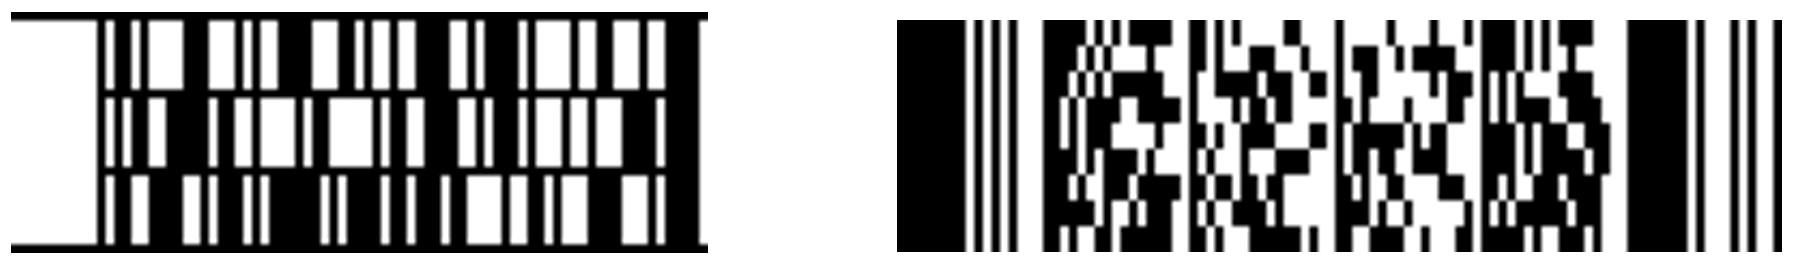
\includegraphics{fig/stackedCodes.PNG}
    } 
    \caption{Skládané dvourozměrné kódy -- Code 49 (vlevo) a PDF417 (vpravo)
    \cite{codeGenerator}}
    \label{stackedCodes}
  \end{center}
\end{figure}

Souběžně se se skládanými kódy vyvíjí i druhá skupina dvourozměrných kódů tzv. 
maticové kódy. Maticové kódy, kam mj. patří i QR kód, jsou tvořeny body, jejichž 
výška a šířka má pevný a stejný rozměr. Pro svůj stejný rozměr kódování 
v horizontálním i vertikálním směru nejsou vertikálně redundantní, tzn. je 
téměř povinnosti využití robustních samoopravných kódů. Naopak díky této 
vlastnosti dokáží uchovat více informací než skládané kódy. Kódy nemusí být 
čteny po řádcích, při jejich čtení se využívá čtecích mřížek. Představiteli 
maticových kódů jsou např. kódy Data Matrix, Aztec Code, MaxiCode aj.
\cite{automatizaceClanek}
             
\begin{figure}[H]
  \begin{center}
    \scalebox{0.20}{
      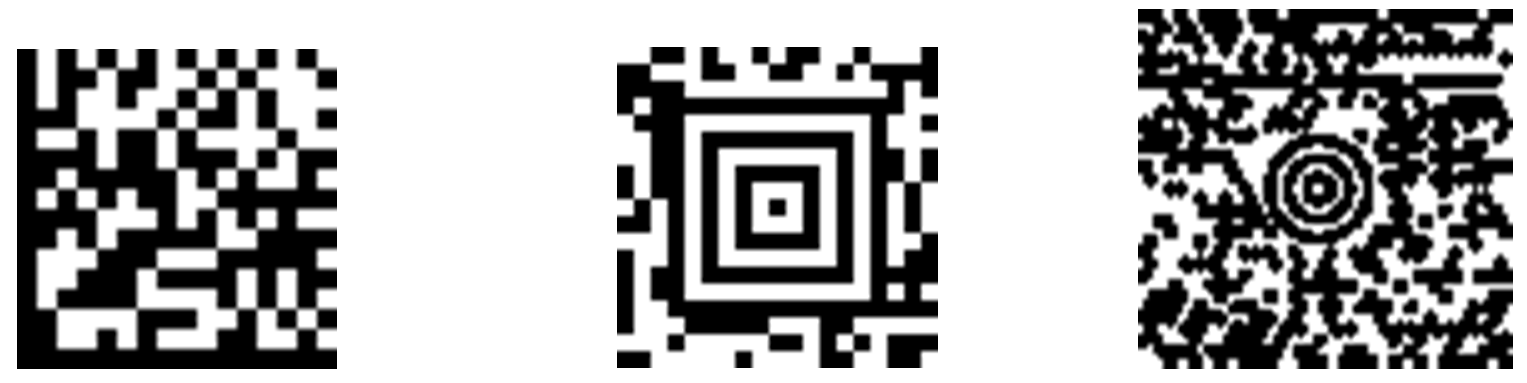
\includegraphics{fig/matrixCodes.PNG}
    } 
    \caption{Maticové dvourozměrné kódy -- Data Matrix, Aztec Code a MaxiCode
    \cite{codeGenerator}}
    \label{matrixCodes}
  \end{center}
\end{figure}              

V současné době již existuje přes 20 různých 2D kódů a stále se vyvíjejí další.
Využívají se především pro značení součástí a výrobků – metoda
DPM\footnote{Direct Part Marking -- přímé značení součástí}.
\cite{automatizaceClanek}


\subsection{Porovnání QR kódů s ostatními 2D kódy}
\label{porovnani2DKoduSQRKody}

QR kódy od ostatních 2D kódů lze rozeznat podle výrazných značek ve třech rozích 
kódu. Tyto značky slouží pro rychlou detekci v rozmanitém okolním prostředí a 
upevnění čtecí mřížky nezávisle na natočení kódu. Mechanismus obnovy, který 
využívají (viz kapitola \ref{metodaReedSolomon}) dokáže obnovit nevalidní a
poničené segmenty dat až do 30 \% poškození (obrázek \ref{corruptedQRCodes}).   

\begin{figure}[H]
  \begin{center}
    \scalebox{0.20}{
      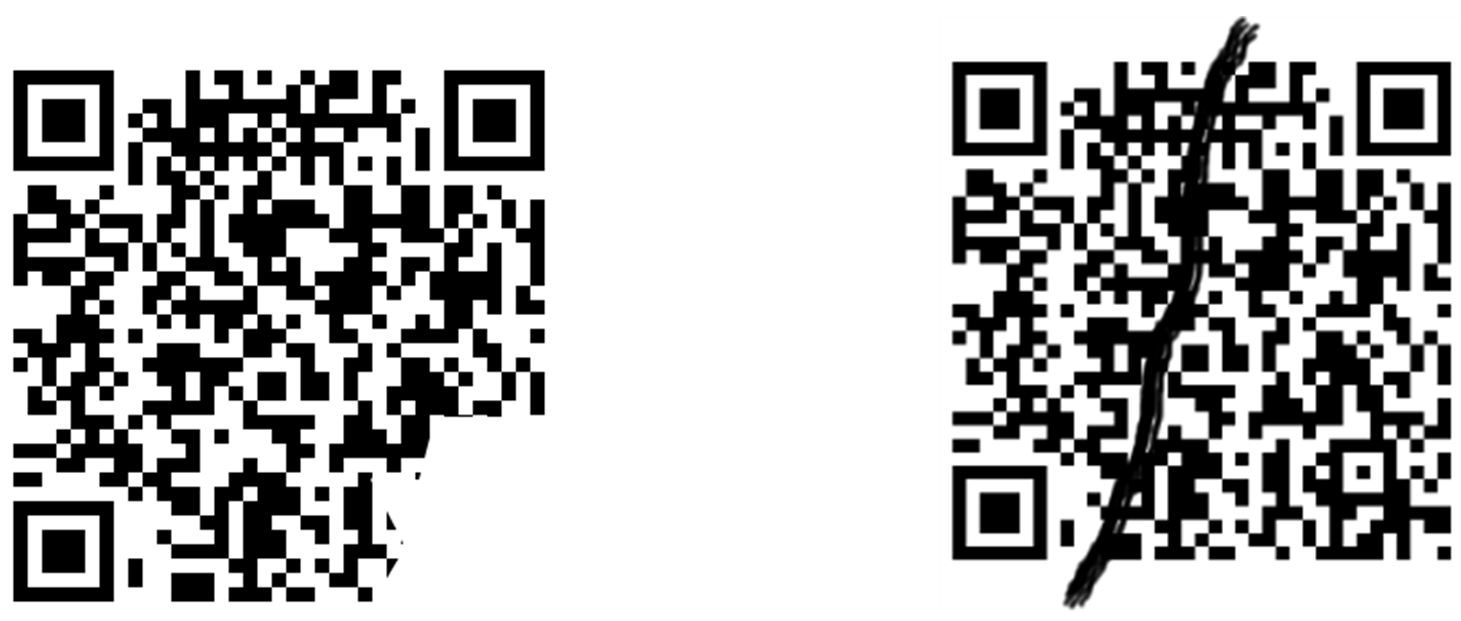
\includegraphics{fig/corruptedQRCodes.PNG}
    } 
    \caption{Ukázka poškozených, ale opravitelných QR kódů}
    \label{corruptedQRCodes}
  \end{center}
\end{figure}

Porovnání s ostatními 2D kódy, zmíněnými v předešlé kapitole
\ref{prehled2DKodu}, lze vidět v následující tabulce \ref{porovnani2DKodu}.

\begin{table}[H]
  \begin{center} 
    \begin{tabular}{| c | c | c | c | c |} \hline
     & \textbf{QR kód} & \textbf{PDF417} & \textbf{Data Matrix} &
     \textbf{MaxiCode} \\
     & (maticový) & (skládaný) & (maticový) & (maticový) \\ \hline
    \textbf{Kapacita režimů} & & & & \\ \hline
    Číselný& 7089 & 2710 & 3116 & 138 \\ \hline
    Alfanumerický & 4296 & 1850 & 2355 & 93 \\ \hline
    Binární & 2953 & 1018 & 1556 & - \\ \hline
    Kanji & 1817 & 554 & 778 & - \\ \hline
     & malé rozměry & \multirow{3}{*}{vysoká kapacita} & \multirow{3}{*}{malé 
     rozměry} & \multirow{3}{*}{rychlost čtení} \\
    \textbf{Výhody} & vysoká kapacita &  &  &  \\
     &rychlost čtení &  &  &  \\ \hline
    \end{tabular}
    \caption{Porovnání dvourozměrných kódů \cite{aboutQRCOde}}
    \label{porovnani2DKodu}
  \end{center}
\end{table}

\subsection{Standardizace QR kódů}
\label{standardizaceQRKodu}

QR kód od své první aplikace v automobilovém průmyslu byl schválen mnoha
standardizačními organizacemi včetně mezinárodních (tabulka 
\ref{standardizaceBehemLet}). Abychom plně porozuměli aktuální mezinárodní normě
ISO/IEC 18004:2006, která strukturu QR kódů aktuálně upravuje, tak se v této 
kapitole podíváme na průběh standardizace, zejména té mezinárodní, trochu blíže.

\begin{table}[H]
  \begin{center} 
    \begin{tabular}{| c | l |} \hline
    \textbf{Datum} & \textbf{Vydaný standard} \\ \hline
    Říjen 1997 & AIM standard (AIM-ITS 97/001) \\ \hline
    Březen 1998 & JEIDA standard (JEIDA-55) \\ \hline
    Leden 1999 & JIS standard (JIS X 0510)  \\ \hline
    Červen 2000 & ISO standard (ISO/IEC 18004:2000) \\ \hline
    Listopad 2004 & 2. vydání normy JIS X 0510 \\ \hline
    Září 2006 & 2. vydání normy ISO 18004 (ISO/IEC 18004:2006)  \\ \hline
    \end{tabular}
    \caption{Standardizace QR kódů v letech \cite{standardizaceDenso}}
    \label{standardizaceBehemLet}
  \end{center}
\end{table}

První mezinárodní norma, která se QR kódy pokusila standardizovat, byla norma 
organizace AIM v roce 1997. Tato norma se snažila držet striktně formy QR kódů, 
které se doposud používaly v aplikačně uzavřeném průmyslovém segmentu, skupinu 
QR kódu sjednotila a položila základy pro ostatní normy. Specifikováno bylo 
celkem 14 verzí QR kódů. Ve 20. století byl QR kód dále standardizován 
japonskými organizacemi JIS a JEIDA a to zejména díky své schopnosti přenášet 
velice výhodně znaky japonských abeced.

V roce 2000 standardizovala QR kódy organizace ISO, přičemž norma vychází 
z normy AIM, kterou ovšem již nedoporučuje dále používat v otevřené 
aplikační sféře. Starou normu AIM značně upravuje, přidává nové a 
odstraňuje staré stavební (konstrukční) prvky\footnote{stavební prvek -- Souhrnné označení pro
ustálené značky a vzory, které nenesou žádná data.}.
Specifikuje celkem 40 verzí QR kódů. Z důvodu kompatibility s normou AIM 
zavádí tzv. rodinu QR kódů, kde staré QR kódy označuje QR kódy modelu 1 a nové
QR kódy modelu 2 (obrázek \ref{QRCodeModel12Comparision}).


\begin{figure}[H]
  \begin{center}
    \scalebox{0.20}{
      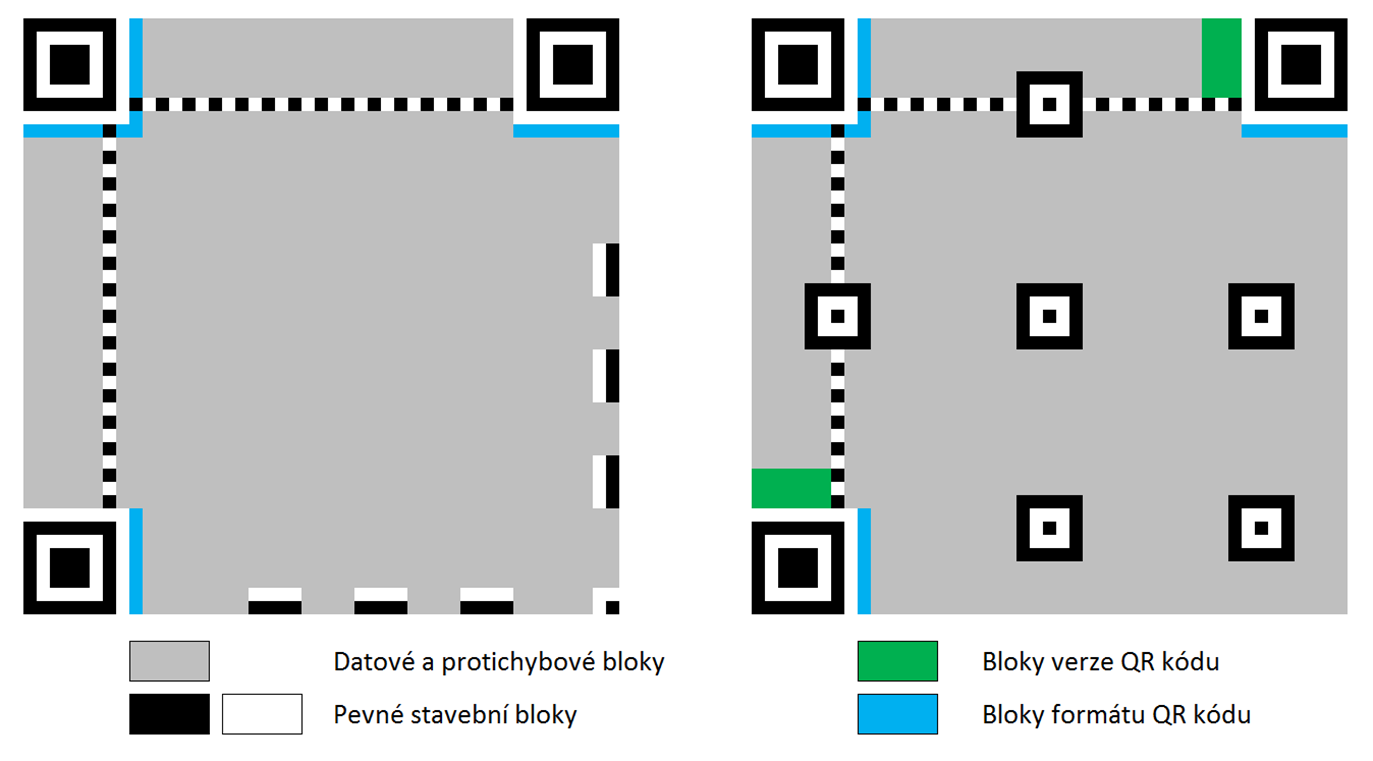
\includegraphics{fig/QRCodeModel12Comparision.PNG}
    } 
    \caption{Porovnaní QR kódu stejné verze modelu 1 (vlevo) a modelu 2 (vpravo)}
    \label{QRCodeModel12Comparision}
  \end{center}
\end{figure}

Aktuální norma ISO/IEC 18004:2006 již přímo vychází z ISO normy vydané v roce 
2000. Nově přidává k rodině QR kódů další dva typy: QR kód 2005 a Micro QR kód. 

QR kód 2005 vychází z QR kódu modelu 2, nepřidává žádné nové stavební prvky 
ani není změněn způsob kódování dat. Od QR kódu modelu 2 se QR kód 2005 
odlišuje zejména v možnostech, jakými může být reprezentován. Byla přidána
 možnost zrcadlení kódu, jeho existence na tmavém povrchu s invertovanými body 
 a možnost specifikace alternativní výchozí znakové sady zakódovaných dat v 
 podobě textu. QR kódy modelu 2 jsou tedy plně kompatibilní s QR kódy 2005. 

Kromě QR kódu 2005 byl v normě ISO/IEC 18004:2006 nově definován Micro QR kód, 
který byl už předtím standardizován v roce 2004 JIS organizací. Tento kód 
se od předešlých kódů liší výrazně -- má velmi malé rozměry a dokáže přenést 
malé množství dat. Z důvodu malých rozměrů se používá často pro značení 
elektrických obvodů a součástek \cite{microQRCodeDenso}. Ale aby přesto mohl o
takto malých rozměrech pojmout co nejvíce dat, značně redukuje počet stavebních
prvků. Norma definuje celkem 4 verze Micro QR kódů značené jako M1 až M4.

\begin{figure}[H]
  \begin{center}
    \scalebox{0.15}{
      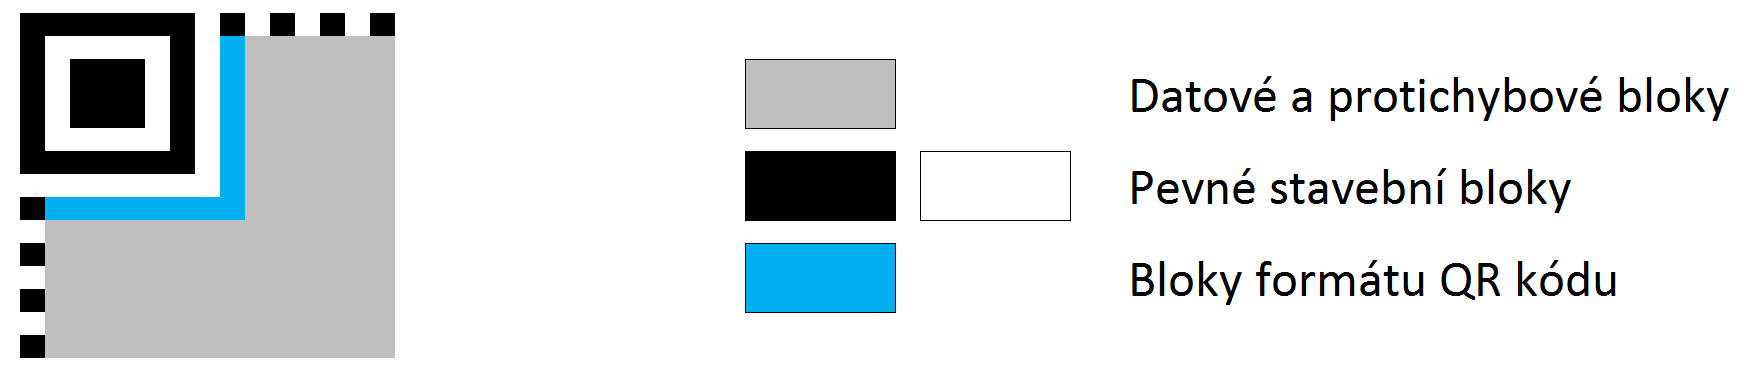
\includegraphics{fig/microQRIntroducion.PNG}
    } 
    \caption{Micro QR kód}
    \label{microQRIntroducion}
  \end{center}
\end{figure}

\section{Struktura QR kódů}
\label{strukturaQRKodu}

QR kód 2005 a Micro QR kód jsou složeny z pevných značek (vzorů), které musí
obsahovat každý kód v dané verzi. Pevné značky jsou umístěny do kódu z důvodu 
rychlé lokalizace kódu, rychlého a věrohodnějšího čtení. Počet pevných značek 
se v závislosti na verzi kódu může měnit. Každý QR kód obsahuje také minimálně
metainformaci o formátu zakódovaných dat. QR kód 2005 pak od verze 7 a výše 
musí obsahovat i metainformaci o své verzi. Každý kód musí být ohraničen 
klidovou zónou, která je alespoň široká jako 4 body kódu.

\begin{figure}[H]
  \begin{center}
    \scalebox{0.25}{
      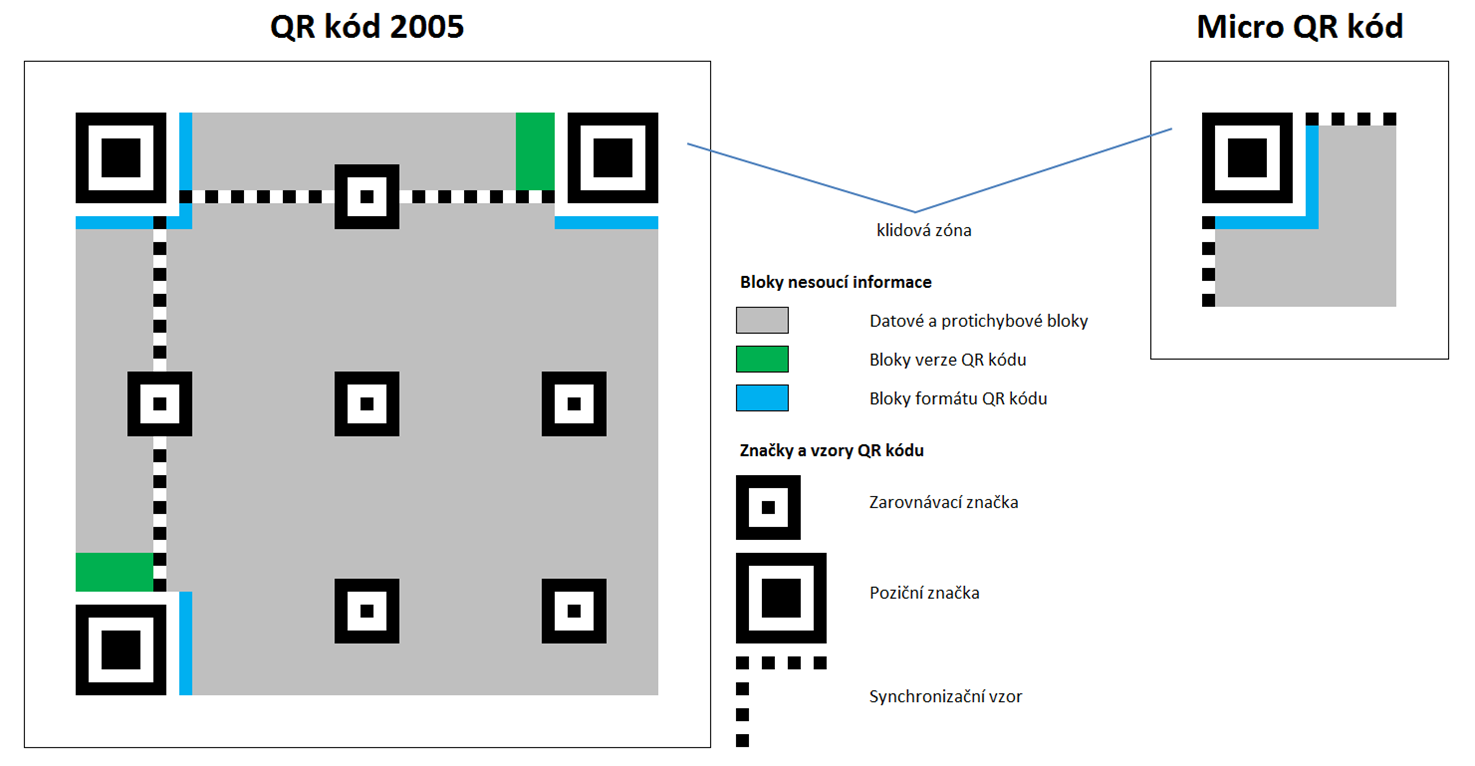
\includegraphics{fig/QRCodesStructure.PNG}
    } 
    \caption{Struktura QR kódu 2005 (znázorněna verze 7)}
    \label{QRCodesStructure}
  \end{center}
\end{figure}

Nejdůležitějšími značkami QR kódů jsou tzv. poziční (lokalizační) značky, které 
slouží pro rychlou lokalizaci kódu v obraze. Rozložení tmavých a světlých bodů 
poziční značky je vertikálně a horizontálně totožné, tmavé body se střídají se 
světlými s poměrem 1:1:3:1:1. Každá poziční značka musí byt oddělena od zóny dat 
pásem světlých bodů. QR kód 2005 obsahuje celkem tři poziční značky, Micro QR 
pouze jednu.

Jelikož kód může být zobrazen v obraze v perspektivní projekci, ale i 
zdeformován zakřiveným povrchem, na kterém je vytištěn, obsahuje kód i 
zarovnávací značky a synchronizační vzory. Tyto prvky slouží pro snadnější 
transformaci kódu z perspektivního či zakřiveného zobrazení do normalizovaného 
zobrazení pro dekódování kódu. Zarovnávací značky jsou umístěny v kódu na 
přesných pozicích, tak jak je definováno v příloze E ISO normy. Micro QR kód 
a QR kód 2005 verze 1 neobsahuje žádné zarovnávací značky. Synchronizační vzory
existují dva, jeden horizontální, druhý vertikální. Oba začínají a končí v pevně
daných pozicích, které jsou totožné v každé verzi QR kódu 2005 a nejinak tomu 
je i u Micro QR kódu. Své uplatnění nachází při odměřování bodů uvnitř datové 
sekce, jejichž polohy lze získat podle středů jednotlivých bodů synchronizačních
vzorů. 

Z hlediska rozměrů má QR kód 2005 verze 1 rozměry 21x21 bodů a každá další verze
rozšiřuje kód předcházející verze o 4 body na výšku i šířku. Z toho plyne, že
verze 40 má rozměry 177x177 bodů. Nejmenší verze Micro QR kódu (M1) začíná na
rozměrech 11x11 bodů, s každou další verzí se rozměry postupně navyšují o dva
body, verze M4 tedy má 17x17 bodů.


\section{Fyzická vrstva}
\label{fyzickaVrstva}

V předcházející kapitole jsme popsali strukturu QR kódu, zmínili jsme se i o
blocích metainformací a datových blocích. V této kapitole se budeme zabývat 
právě formátem a způsobem kódování informací, které jsou obsažené v těchto 
blocích, ale také i samotným dekódováním, které bude poté využito při tvorbě 
čtečky QR kódů.

\subsection{Formát a kódování metainformací}
\label{formatMetainformaci}

Samotná informační data metainformací nejsou kódována žádným kódem, nicméně 
každý blok s metainformacemi obsahuje také bity kontroly a korekce chyby a právě
pro jejich výpočet je zapotřebí využít kódování BCH --
Bose-Chaudhuri-Hocquenghem (viz příloha \ref{ukazkaVypoctuECCMetainformace}).

Z důvodu malého počtu možných kombinací, které mohou BCH kódováním vzniknout, a 
náročnosti výpočtu kódu, je vhodné si pro kódování i dekódování metainformací 
vytvořit vyhledávací tabulku. Pro dekódování norma použití vyhledávací tabulky 
přímo doporučuje. Jelikož je minimální Hammingova vzdálenost pro použité 
samoopravné BCH kódy v obou metainformacích rovna tří, lze během čtení 
metainformací opravit maximálně tři bitové chyby. V případě využití vyhledávací 
tabulky nám tedy stačí nalézt záznam, který se shoduje v nejvíce bitech a přitom
se liší maximálně ve třech bitech.


\subsubsection{Formát metainformace verze QR kódu}
\label{metainfoVersionEncoding}

Přikládat do QR kódu blok s metainformací o verzi kódu požaduje norma pouze pro
QR kódy 2005 od verze 7 a výše. Jedinou informací, kterou tento blok nese je 
informace o verzi QR kódu, která je v něm uložena jako číslo na šesti bitech. 
Zbylé bity bloku jsou bity korekce chyby (ECC), které jsou k samotnému číslu 
na závěr připojeny. Metainformace verze QR kódu je uložena vedle dvou pozičních 
značek redundantně.

\begin{figure}[H]
  \begin{center}
    \scalebox{0.15}{
      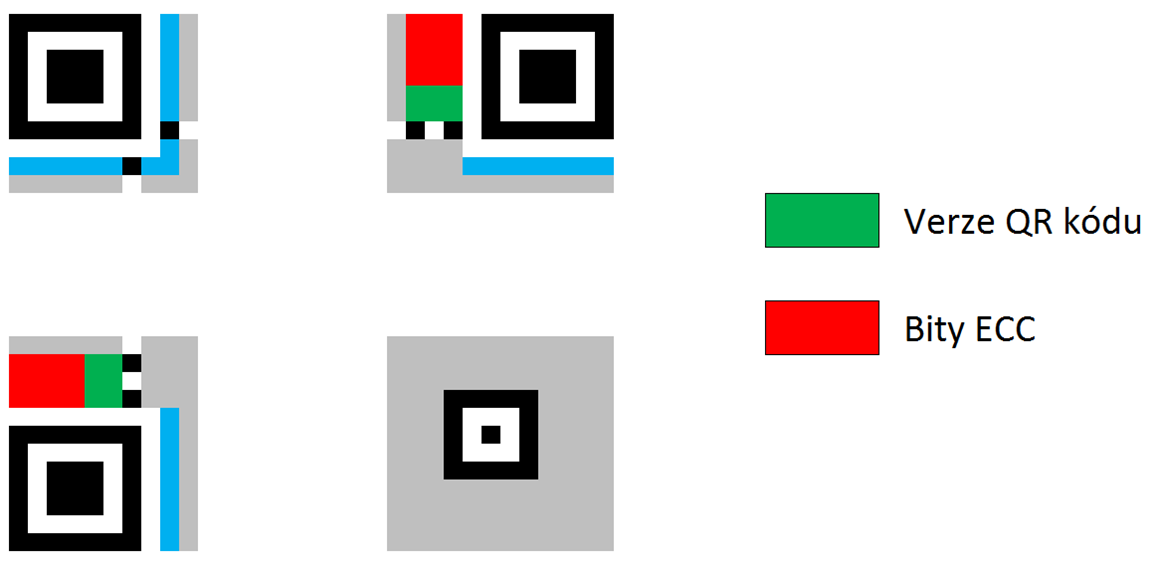
\includegraphics{fig/QRCodeVersionMetainformation.PNG}
    } 
    \caption{Znázornění bloků s metainformací verze QR kódu}
    \label{QRCodeVersionMetainformation}
  \end{center}
\end{figure}

\subsubsection{Formát metainformace formátu dat}
\label{metainfoFormatEncoding}

Každý QR kód, již od modelu 1, má blok s metainformací o způsobu zakódování
výsledného vzoru dat. 

V případě QR kódu 2005 tento blok obsahuje informaci o 
úrovni použité korekce chyb (2 bity), kterou kód disponuje (viz kapitola 
\ref{metodaReedSolomon} tab. \ref{moznostiZotaveniTabulka}). Druhým údajem,
který v bloku můžeme nalézt, je informace o masce (3 bity), která byla na
výsledný vzor s daty aplikována za účelem odstranění nežádoucích vzorů z dat
podobajících se pozičním značkám (viz kapitola \ref{tvorbaVystupnihoVzoru} obr.
\ref{QRCodeDataMasks}).

Micro QR kód blok metainformace také využívá 
pro uložení informace o masce (pouze 2 bity), ale jako druhou informaci přenáší 
číslo kódu (3 bity), které v sobě zapouzdřuje úroveň použité korekce chyby a 
samotnou verzi Micro QR kódu.

\begin{figure}[H]
  \begin{center}
    \scalebox{0.15}{
      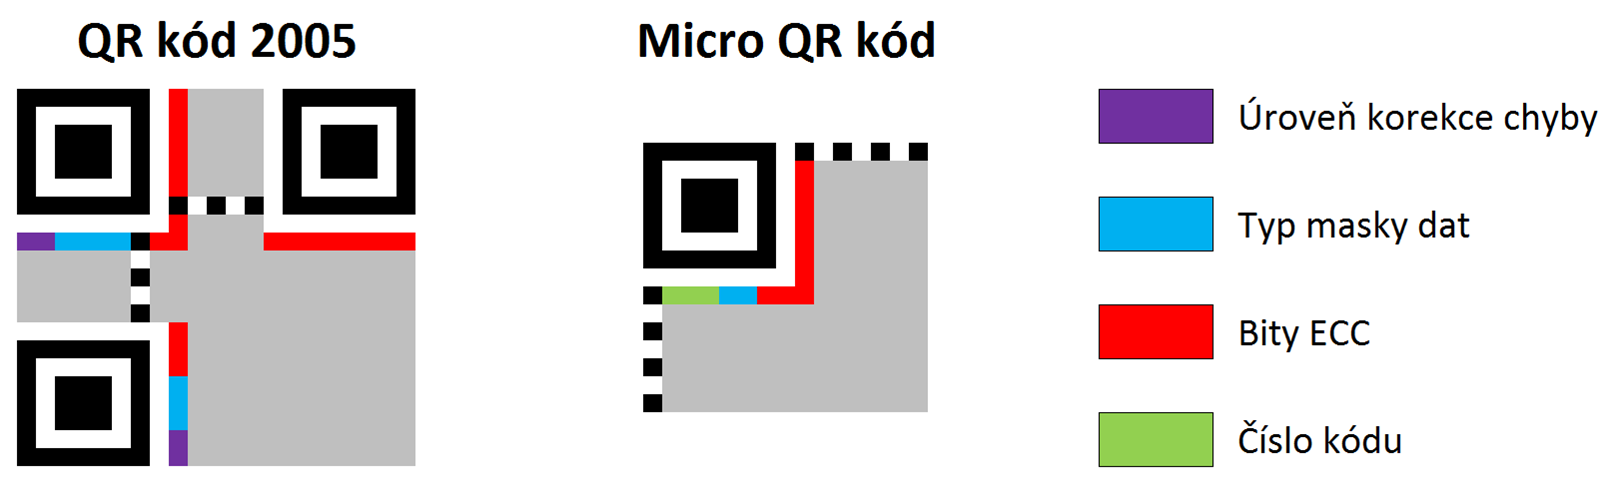
\includegraphics{fig/QRCodeFormatMetainformation.PNG}
    } 
    \caption{Znázornění bloků s metainformací formátu QR kódu}
    \label{QRCodeFormatMetainformation}
  \end{center}
\end{figure}

\subsection{Kódování dat}
\label{kodovaniDat}

Datový proud, jenž má být QR kódem přenášen, by neměl být vložen do kódu přímo,
nýbrž zapouzdřen do jednoho či více datových segmentů. Datové segmenty přitom 
mohou být řazeny v závěsu za sebe. Každý segment musí v hlavičce obsahovat své
unikátní označení tzv. indikátor režimu. Segmentování v čárových kódech slouží
k efektivnějšímu přenosu specifických typů dat, jako jsou řetězce čísel,
alfanumerických či znaků japonských abeced. Zatímco ve znakovém režimu bychom
mohli přenést na 3 bytech pouze 3 cifry, v numerickém režimu jich můžeme přenést
celkem 9.  Celá sekvence segmentů musí být zakončena speciálním segmentem tzv.
terminátorem.

\begin{figure}[H]
  \begin{center}
    \scalebox{0.25}{
      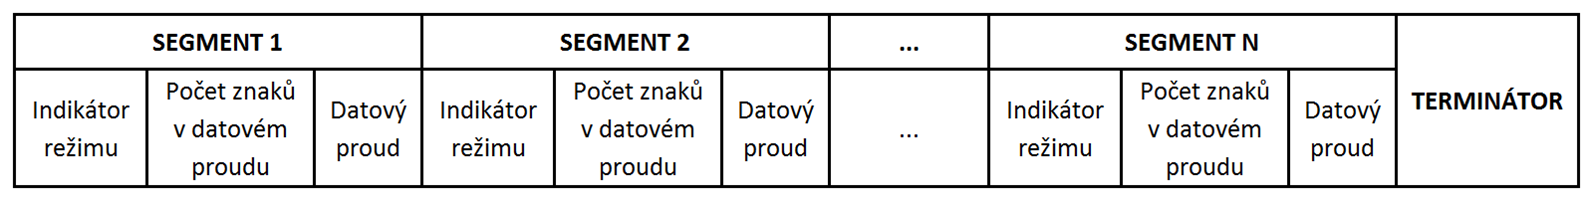
\includegraphics{fig/QRCodeDataSegments.PNG}
    } 
    \caption{Ukázka kódování dat do datových segmentů}
    \label{QRCodeDataSegments}
  \end{center}
\end{figure}

\bigskip \noindent Pro QR kódy existují následující režimy (typy segmentů): 
\begin{itemize}
  \item \textbf{numerický} -- slouží pro přenos čísel, číslice se snaží kódovat
 do skupin o třech cifrách a přenášet je na 10 bitech. Obsahuje-li skupina méně 
 než 3 cifry, poté jsou přenášeny tyto cifry na 7 nebo 4 bitech;
  \item \textbf{alfanumerický} -- přenáší alfanumerické znaky a některé další 
  symboly -- celkem 45 znaků;
  \item \textbf{binární} -- nespecifikuje datům žádnou sémantiku a přenáší je po
  bytech;
  \item \textbf{Kanji} -- efektivně kóduje znaky japonských abeced;
  \item \textbf{ECI} -- režim neslouží pro přenos dat, nýbrž pro specifikaci
  kódové sady znaků v~následujících segmentech. Výchozí sadou je ISO/IEC 8859-1;
  \item \textbf{FNC1} -- FNC1 režim nepřenáší data, pouze značí, že následovaná
  data podléhají specifickému kódování EAN.UCC nebo jinému registrovanému AIM organizaci;
  \item \textbf{strukturovaný} -- pokud je segment s tímto režim obsažen v QR 
  kódu, říká nám, že data v jeho závěsu jsou neúplná a rozdělena do více QR 
  kódů. Pro sestavení a uspořádání kompletních dat poté slouží sekvenční 
  číslo, které je zahrnuto v každém strukturovaném segmentu.
\end{itemize}

\subsection{Metoda zotavení z chyb Reed-Solomon}
\label{metodaReedSolomon}

Pro zotavení dat z chyb je v QR kódech využívána bloková a nebinární
Reed-Solomon (RS) kódovací metoda. Mimo QR kódů se s ní můžeme setkat např. u 
 CD a DVD nosičů, ADSL, mobilních telefonů, mezisatelitní komunikace či 
televizního přenosu DVB. Reed-Solomon metoda má podklad v diskrétní matematice 
a kódy, které generuje, se dají vyjádřit cyklickým posunem a lineární kombinací
jiného kódového slova. Jedná se tedy o lineární a cyklický kód.

Reed-Solomonovy kódy (RS kódy) vznikly specializací BCH kódů. Jejich sestavení
se uskutečňuje pomocí operací využívajících prvků Galoisova tělesa $GF(2^m)$. 
Jelikož se jedná o nebinární kódování, pracuje RS kódovací metoda pouze se 
symboly (nikoliv bity), jež vstupují do dekódovacího procesu a mohou být také 
opraveny. Těleso $GF(2^m)$ je poté rozšířením binárního tělesa $GF(2)$ a ke
dvěma prvkům abecedy $\{0,1\}$ přidává další prvky vyjádřené jako mocniny
primitivního prvku $\alpha$ (pro QR kódy $\alpha = 2$): 

\begin{equation}
  F = \{ 0, 1, \alpha^1, \alpha^2, \ldots, \alpha^{2^{m}-4}, \alpha^{2^{m}-3},
  \alpha^{2^{m}-2}\}\mbox{.}
\end{equation}

\noindent V případě QR kódů obsahuje vždy Galoisovo těleso $2^8$ prvků, neboť
kódové symboly QR kódu jsou 8 bitů dlouhé. \cite{sklarRSCodes}

Výsledný RS kód je tvořen generujícími polynomy 
$g(x)$ stupně $n-k$, kde $n$ je délka výsledného kódu a $k$ délka nezakódovaných 
informačních dat. Vždy přitom musí platit, že generující polynom dělí polynom 
$x^n-1$ beze zbytku. Pro QR kódy jsou již v závislosti na $k$ i $n$ generující 
polynomy sestaveny (viz ISO norma příloha A).

Pokud uvážíme informační data v polynomiálním tvaru
\begin{equation}
  f(x) = f_{0} + f_{1}x + f_{2}x^2 + \ldots + f_{n-1}x^{n-1}\mbox{,}
\end{equation}
\noindent výsledná paritní část informačních dat, jež je k datům na závěr
připojena, je zjistitelná vztahem

\begin{equation}
  \frac{f(x) x^{n-k}}{g(x)} = h(x) + \frac{r(x)}{g(x)}
\end{equation}

\noindent jako zbytek po dělení $r(x)$. \cite{decodingRSCodesLiterature}

V praxi se pro generování kódu vyžívá generující neboli bázové matice
$\mathbf{G(x)}$ (rovnice \ref{generujiciMatice}), která vychází z cyklických a
lineárních vlastností RS kódu.
Matice má celkem $k$ lineárně nezávislých řádků, které jsou tvořeny cyklicky posunutými kódovými 
slovy. Výsledný kód je poté zjištěn pomocí lineární kombinace jednotlivých 
řádků matice. \cite{hallBCH}

\begin{equation}
  \mathbf{G} = \left(
    \begin{array}{cccccccccccc}
      g_{n-k} & g_{n-k-1} & \ldots & \ldots & \ldots & \ldots & g_{1} & g_{0} &
      0 & 0 & \ldots & 0 \\
      0 & g_{n-k} & g_{n-k-1} & \ldots & \ldots & \ldots & \ldots & g_{1} &
      g_{0} & 0 & \ldots & 0 \\
      \vdots & \vdots & \ddots & \ddots & \ddots & \ddots & \ddots & \ddots &
      \ddots & \ddots & \ddots & \vdots \\
      0 & 0 & \ldots & 0 & g_{n-k} & g_{n-k-1} & \ldots & \ldots & \ldots &
      \ldots & g_{1} & g_{0} \\
    \end{array}
  \right)
  \label{generujiciMatice}
\end{equation}

Proces dekódování a případné opravy chyby v RS kódu je více komplikovaný a jeho
popis by překračoval rozsah této práce. Jeho základní podstata je vystižena v
diagramu na obrázku \ref{ReedSolomonDecodingProcess}. Pro určení chybového
polynomu existuje více metod, z těch efektivnějších můžeme jmenovat Euklidovský nebo Berlekampův algoritmus. 
Během řešení kořenů chybového mnohočlenu se může uplatnit algoritmus Chienova 
vyhledávání a při zjišťování velikosti chyby Forneyův algoritmus.
\cite{decodingRSCodesLiterature}

\begin{figure}[H]
  \begin{center}
    \scalebox{0.22}{
      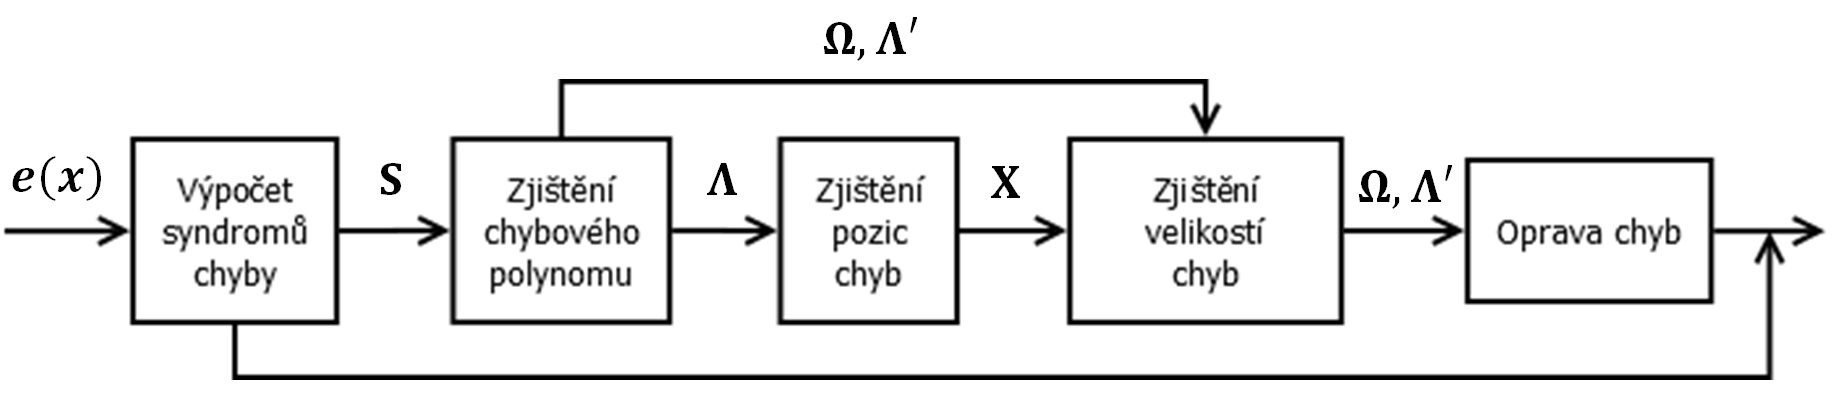
\includegraphics{fig/ReedSolomonDecodingProcess.PNG}
    } 
    \caption{Proces dekódování Reed Solomon kódu}
    \label{ReedSolomonDecodingProcess}
  \end{center}
\end{figure}

Podmínka opravitelnosti RS kódu, kde $t$ je počet
detekovaných chyb, je dána: \cite{sklarRSCodes}

\begin{equation}
  t \leq \frac{n - k}{2}\mbox{.}
\end{equation}

Data v QR kódech mohou být zabezpečena čtyřmi různými úrovněmi L, M, Q a H
(tabulka \ref{moznostiZotaveniTabulka}). Z pohledu RS kódů změna úrovně
zabezpečení znamená zvolení jiné délky $n$ pro výslednou kódovou zprávu, přičemž délka zprávy nesmí přesáhnout 
$2^m+1$ symbolů, neboť pro RS kódy platí: \cite{sklarRSCodes}

\begin{equation}
  0 < k < n < 2^{m} + 2\mbox{.}
\end{equation}

Aby byla předchozí podmínka splněna, jsou pro větší QR kódy datové segmenty
rozděleny do bloků a zabezpečení probíhá nad více vzájemně nezávislými bloky
(viz ISO norma tabulka 9)

\begin{table}[H]
  \begin{center} 
    \begin{tabular}{| c | c |} \hline
    \textbf{Úroveň korekce chyb} & \textbf{Možnost zotavení z chyb (cca \%)} \\ \hline
    L & 7 \\ \hline
    M & 15 \\ \hline
    Q & 25 \\ \hline
    H & 30 \\ \hline
    \end{tabular}
    \caption{Možnosti zotavení dat v procentech}
    \label{moznostiZotaveniTabulka}
  \end{center}
\end{table}

Aktuální aplikovaná úroveň zabezpečení pro daný kód je uložena v metainformaci
formátu QR kódu. Zatímco QR kódy 2005 mohou pro svůj přenos využít všechny 4 
úrovně, u Micro QR kódu je schopnost zabezpečení závislá na verzi kódu. Pro 
verzi M1 např. neexistuje žádné zotavení z chyby, pouze detekce chyby, a vyjma 
verze M4 nepodporují Micro QR kódy korekci úrovně Q.

\subsection{Tvorba výstupního vzoru}
\label{tvorbaVystupnihoVzoru}

\begin{figure}[H]
  \begin{center}
    \scalebox{0.50}{
      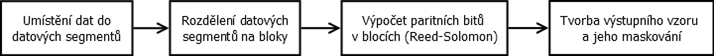
\includegraphics{fig/CreatingOutputPatternProcess.PNG}
    } 
    \caption{Kroky vedoucí ke tvorbě výstupního vzoru}
    \label{CreatingOutputPatternProcess}
  \end{center}
\end{figure}

Pokud máme data vložena do datových segmentů s vhodně zvolenými režimy pro 
přenos (kapitola \ref{kodovaniDat}), datové segmenty rozděleny na bloky a vypočítány pro
ně paritní bity korekce (kapitola \ref{metodaReedSolomon}), můžeme přistoupit k finálnímu
umístění bloků do QR kódu.

Kódová slova bloků jsou umísťována do QR kódu vertikálně v šíři 2 bodů od 
pravého dolního rohu směrem do levého horního rohu, přičemž po dosažení 
horní či dolní strany je směr zápisu zrcadlen. Kódová slova korekce jsou 
vždy z bloků vytržena a umísťována do kódu až po zápisu všech kódových 
slov dat. Pakliže musíme umístit více než jeden blok, je zapotřebí uplatnit 
prokládání kódových slov mezi bloky. Velikost prokládání je rovna počtu všech 
bloků a slouží pro rovnoměrné rozložení případných chyb do více nezávisle 
zabezpečených bloků. 

Pokud bychom uvážili QR kód verze 5 s úrovní korekce H, 
tento kód má celkem 4 zabezpečené bloky, kde první dva bloky obsahují 11 
kódových slov dat a 22 kódových slov korekce, zbylé dva bloky obsahují akorát 
o 1 kódové slovo dat více, budou kódová slova vkládána do QR kódu tak, jak 
lze vidět na následujícím obrázku \ref{PuttingDataCodewordsIntoQRCode}.

\begin{figure}[H]
  \begin{center}
    \scalebox{0.35}{
      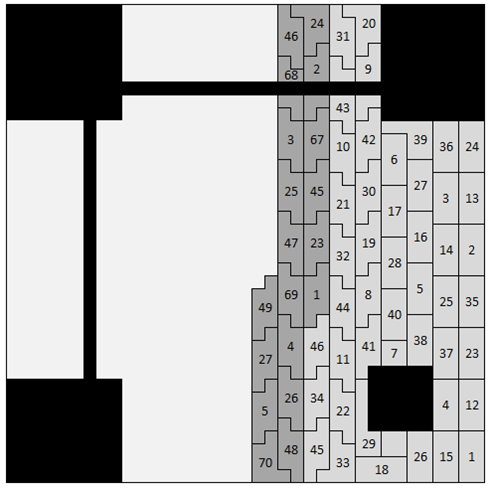
\includegraphics{fig/PuttingDataCodewordsIntoQRCode.PNG}
    } 
    \caption{Znázornění způsobu organizace kódových slov v QR kódu}
    \label{PuttingDataCodewordsIntoQRCode}
  \end{center}
\end{figure}

Po umístění kódových slov do kódu nám zbývá pouze zvolit vhodnou masku pro
případné odstranění lokalizačních značek (vzorů) ze vzoru s daty. Pro QR kód
2005 je definováno celkem 8 masek a pro Micro QR kód 4 masky. Vyhodnocení
nejvhodnější masky probíhá otestováním všech masek nad vzorem s daty a vybrání
té s nejlepšími vlastnostmi. Maskování je založeno na aplikaci operace XOR nad
jednotlivými body QR kódu a body masky.

\begin{figure}[H]
  \begin{center}
    \scalebox{0.18}{
      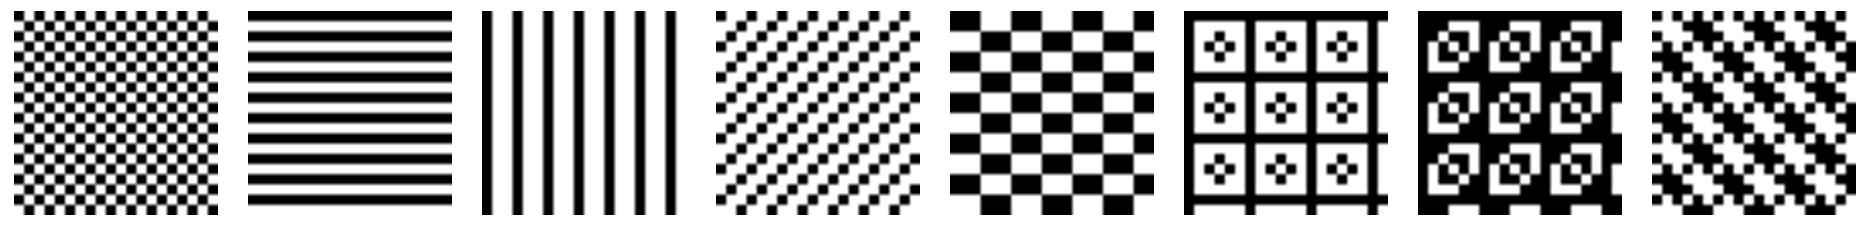
\includegraphics{fig/QRCodeDataMasks.PNG}
    } 
    \caption{Sada datových masek QR kódu}
    \label{QRCodeDataMasks}
  \end{center}
\end{figure}

\section{Aplikační vrstva}
\label{aplikacniVrstva}

Aplikační vrstva pro import informací do mobilních telefonů přenášenými QR kódy 
není nijak standardizována a může být vždy specifická pro danou aplikaci. 
Postupem času se ustálily především dva univerzální formáty, které si zde 
zmíníme.

\bigskip \noindent Prvním způsobem, jak přenášet informace, je kódovat je do URI
\cite{zxingContents,sixrevisionsURI}:

\begin{verbatim}
             schéma: hierarchická část [?dotaz] [#fragment]
\end{verbatim}

Používaná URI schémata, jež jsou registrována organizací IANA, lze vidět v
tabulce \ref{URISChemes}. Vyjma těchto schémat se můžeme setkat ale i
neregistrovanými schématy \texttt{URL}, \texttt{SMSTO} aj.

\begin{table}[H]
  \begin{center} 
    \begin{tabular}{| c | c | l |} \hline
    \textbf{Přenos} & \textbf{Norma} & \textbf{Formát přenášených dat} \\ \hline
    SMS & RFC 5724 & \texttt{sms:+15105550101?body=hello\%20there} \\ \hline
    webové stránky & RFC 2616 & \texttt{http://www.example.com} \\ \hline
    e-mailu & RFC 6068 & \texttt{mailto:chris@example.com} \\ \hline
    polohy & RFC 5870 & \texttt{geo:13.4125,103.8667} \\ \hline
    tel. čísla & RFC 3966 & \texttt{tel:+19005550191} \\ \hline
    \end{tabular}
    \caption{Používaná a registrovaná schémata organizací IANA}
    \label{URISChemes}
  \end{center}
\end{table}

Druhým způsobem pro přenos informací je využití metodiky firmy NTT DoCoMo
\cite{DOCOMOFormatsLiterature}, která definuje formáty zejména pro vytváření
záložek URL adres, přenos kontaktů a elektronických zpráv (Tabulka
\ref{DOCOMOFormatsTable}). Pro přenos kontaktu se můžeme setkat i s formátem
vCard (viz RFC 6350).

\begin{table}[H]
  \begin{center} 
    \begin{tabular}{| c | l |} \hline
    \textbf{Přenos} & \textbf{Formát přenášených dat} \\ \hline
    webové záložky & \texttt{MEBKM:URL:example.com;TITLE:Example;;} \\ \hline
    e-mailu & \texttt{MATMSG:TO:nick@example.org;SUB:subject;BODY:body;;}\\
    \hline kontaktu & \texttt{MECARD:TEL:+123456789;N:John
    Black;URL:example.com;;} \\ \hline
    \end{tabular}
    \caption{Příklady využití formátu firmy NTT DoCoMo}
    \label{DOCOMOFormatsTable}
  \end{center}
\end{table}

\section{Čtení QR kódů}
\label{refCteniQRKodu}

Pro čtení QR kódů aktuální ISO norma definuje referenční algoritmus, který je
možné použít, ovšem není nutný, při tvorbě čtečky QR kódů. Základní kroky 
algoritmu, které lze považovat za obecné a uplatní se při tvorbě všech čteček 
QR kódů, můžeme vidět ve vývojovém diagramu na obrázku
\ref{QRCodeReferenceReadingProcess}.

\begin{figure}[H]
  \begin{center}
    \scalebox{0.27}{
      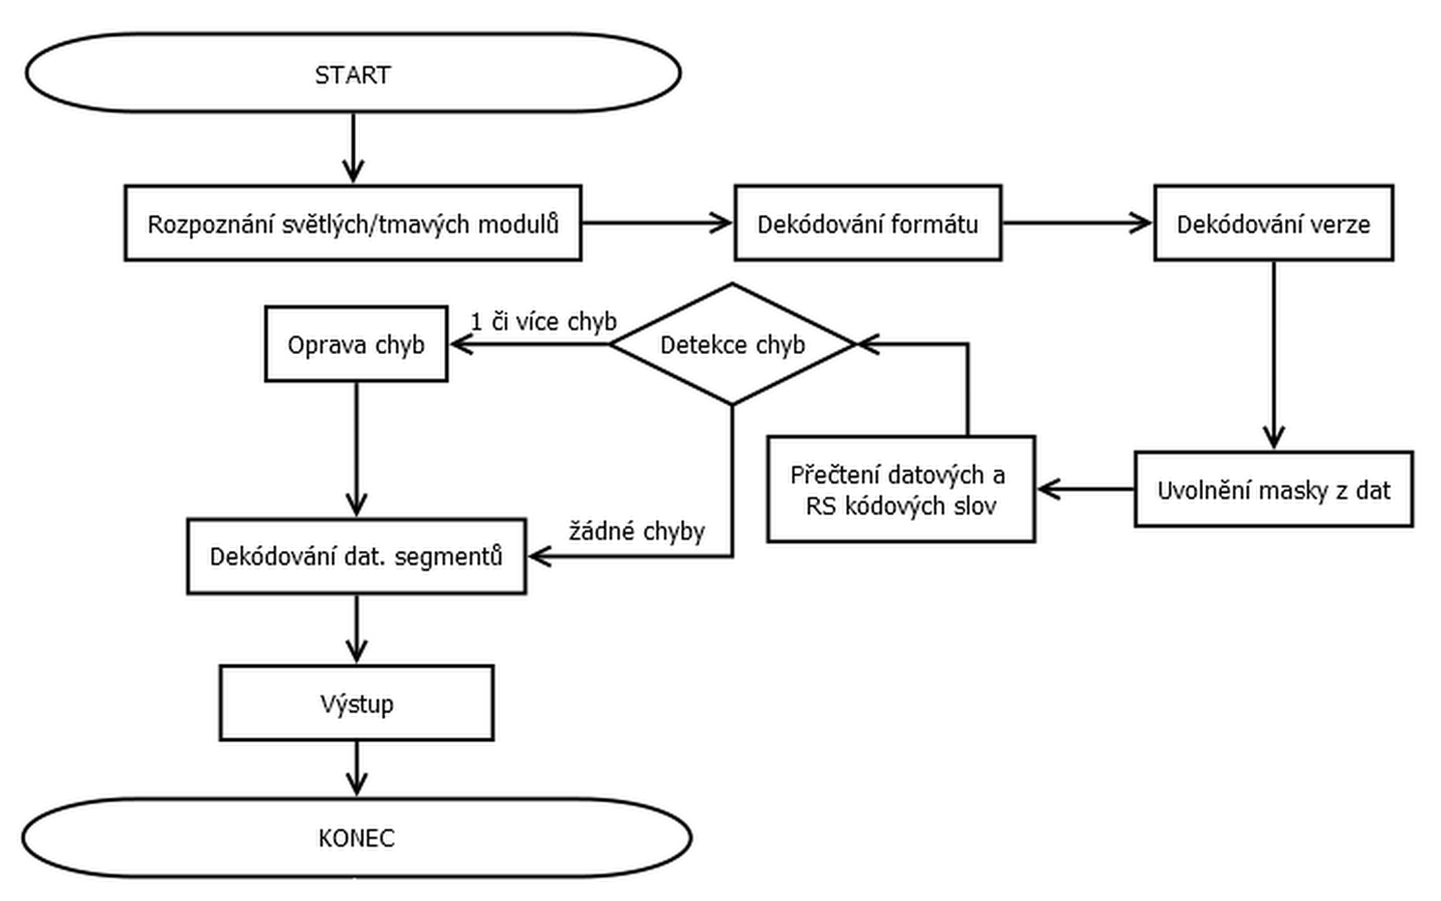
\includegraphics{fig/QRCodeReferenceReadingProcess.PNG}
    } 
    \caption{Referenční vývojový diagram znázorňující kroky čtení QR kódu}
    \label{QRCodeReferenceReadingProcess}
  \end{center}
\end{figure}

Jednotlivé kroky předešlého vývojového diagramu jsou ve znění referenčního
algoritmu upřesněny. My si je zde ale nebudeme popisovat a pokusíme se nalézt 
v návrhu čtečky QR kódu vlastní, příp. modifikovaný algoritmus.

\chapter{Google Android}
\label{android}

Android je open-source softwarová platforma vyvíjená zejména pro mobilní
zařízení. Zahrnuje v sobě operační systém, podpůrný systém pro běh aplikací 
a některé klíčové aplikace.

\section{Architektura}
\label{AndroidArchitektura}

Tato podkapitola čerpá z \cite{whatISAndroid}. Základní
architektura platformy Android se skládá z aplikační vrstvy, aplikačního frameworku, knihoven, Androidu runtime a Linuxového jádra.
Přehledně ji můžeme vidět na následujícím obrázku:

\begin{figure}[H]
  \begin{center}
    \scalebox{0.35}{
      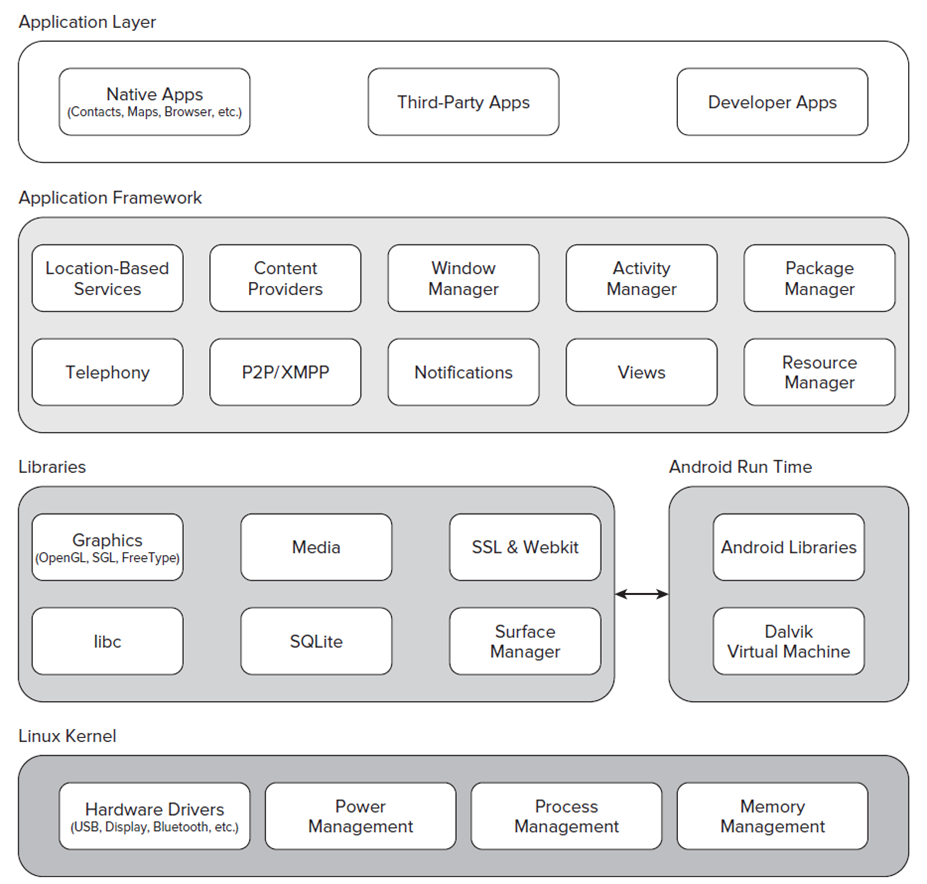
\includegraphics{fig/AndroidArchitecture.PNG}
    }
    \caption{Architektura platformy Android \cite{AndroidProfessionals}}
    \label{AndroidArchitecture}
  \end{center}
\end{figure}

\textbf{Aplikační vrstva}, nejvyšší vrstva abstrakce, tvoří prostor pro běh
aplikací. Zařízení používající Android jsou zpravidla dodávána již se sadou
předinstalovaných optimalizovaných aplikací. Bývají jimi být např. webový prohlížeč, aplikace na zpracování obrazu z~kamery, SMS a e-mailový klient aj. Všechny aplikace v této vrstvě jsou napsány v jazyce Java a jsou spouštěny na speciálním virtuálním stroji zvaném Dalvik.

\bigskip \textbf{Aplikační framework} nabízí vývojové prostředky pro tvorbu aplikací
v aplikační vrstvě. API frameworku poskytuje plný přístup ke stejným komponentám, které používají klíčové aplikace systému. Architektura tvorby aplikací je založena na opětovném využívání komponent, které mohou být každou aplikací zveřejněny. Obdobný systém umožňuje i komponenty nahrazovat.

\bigskip \textbf{C/C++ knihovny} poskytují zázemí pro běh některých klíčových
API komponent, ale také samotného virtuálního stroje, proto musí být vždy
součástí distribuce platformy. Hlavními knihovnami jsou: standardní systémová knihovna C (libc), knihovny pro práci s~médii a grafikou (SGL, OpenGL, FreeType), relační databázový systém (SQLite) a další.

\bigskip \textbf{Android runtime} obsahuje sadu klíčových knihoven,
zajišťujících většinu funkcionality pro interpretaci jazyka Java, a samotný
virtuální stroj Dalvik. Každá třída, která má být spuštěna pomocí virtuálního
stroje musí být převedena do formátu Dalvik Executable (.dex) pomocí nástroje
\texttt{dx}, jež je přístupný v Android SDK. Aplikace jsou vždy
spouštěny jako nový proces s vlastní instancí virtuálního stroje.

\bigskip \textbf{Linuxové jádro} platformy Android je verze 6 a zprostředkovává
služby zabezpečení, správu paměti, správu procesů, ovladačů aj.

\section{Aplikace}

Aplikace pro Android jsou psány v jazyce Java, přičemž pro spuštění musí být
zkompilovány do formátu Dalvik Executable. Pro distribuci by měly být aplikace
zabaleny do balíku s příponou \texttt{.apk} a podepsány certifikátem. Při
podepisování se využívá asymetrického šifrování, vlastníkem privátního klíče je sám autor
aplikace. Nové aplikace je zapotřebí vždy nainstalovat, během níž se každé
aplikaci přiřadí vlastní uživatelský účet, s nímž bude spouštěna, vytvoří
privátní složka pro ukládání souborů a balík s kompilovaným kódem aplikace
překopíruje do systémových složek Androidu.

\subsection{Komponenty aplikace}

Tato podkapitola čerpá z \cite{applicationAndroidFundamentals}. Komponenty
aplikace jsou základními stavební bloky pro tvorbu aplikací na platformě Android. O jejich existenci informujeme systém během instalace ve
speciálním XML souboru (\texttt{AndroidManifest.xml}), který je nutno umístit do
\texttt{.apk} archivu. Komponenty tvoří jakési přístupové a spouštěcí body,
jejich kód je systémem vyvoláván na základě nějaké vnější události. Aktuálně
existují celkem 4 druhy komponent: \texttt{Activity}, \texttt{Content Provider},
\texttt{Service} a \texttt{Broadcast receiver}.

\bigskip \textbf{Activity} komponenta představuje jednoduchou
obrazovku, na které lze vytvářet aplikace s uživatelským rozhraním. Tuto
komponentu lze vyvolat metodou \texttt{startActivity()}. Pokud se dostane do
popředí jiná Activity, aktuálně spuštěná Activity je pozastavena a může být uvolněna i z paměti a její stav uložen.

\bigskip \textbf{Service} komponenta neposkytuje uživatelské rozhraní,
běží jako služba na pozadí systému bez vědomí uživatele a lze jí spustit metodou
\texttt{startService()}.

\bigskip \textbf{Broadcast receiver} komponentou můžeme zachytávat
vyslaná veřejná oznámení jinými komponentami. Komponenta, která vysílá veřejné
oznámení, volá \texttt{sendBroadcast()}.

\bigskip \textbf{Content provider} je speciální komponenta, která
dokáže zprostředkovávat soukromá data aplikace jiným aplikacím.

\bigskip Invokace komponent (mimo \texttt{Content provider}) probíhá pomocí
objektů instance \texttt{Intent}. Komponenta může být zavolána buď přímo, pokud známe
její třídu, která komponentu implementuje, nebo nepřímo požadavkem, jež lze 
předat \texttt{Intent} instancí. Jaké druhy požadavků může komponenta zpracovat
lze oznámit systému opět manifest souborem elementem \texttt{<intent-filter>}.


\chapter{Návrh}
\label{navrh}

V této kapitole budeme nejprve diskutovat požadavky pro cílovou aplikaci a
stanovíme si cíle, jichž budeme chtít dosáhnout. Dále si popíšeme, jakými 
vhodnými způsoby lze lokalizovat QR kód v obraze a přečíst jeho obsah. 
Aktuální ISO norma sice uvádí referenční postup jak QR kódy číst, ale neuvádí 
konkrétní algoritmy a metody zpracování obrazu, jakými toho docílit. Z tohoto
důvodu se pokusíme v této kapitole tyto metody navrhnout a upřesnit. Závěrem
kapitoly bude prezentován základní návrh architektury aplikace.

\section{Stanovení cílů}

Pro návrh algoritmů detekce a čtení je zapotřebí zohlednit aplikační doménu, ve
které budou pracovat, a podporované QR kódy, které budou schopny zpracovat.

Víme, že aplikace bude tvořena pro čtení QR kódu mobilními přístroji, QR kód
se tedy bude nacházet v prostoru a v perspektivním zobrazení. V rámci přípravy
obrazu pro čtení bude nutno provést transformaci do normalizovaného zobrazení
(kapitola \ref{inverzniPerspektivniTransformace},
\ref{detekcePozicnichZnacek}, \ref{zjisteniATransformace}). Snímání obrazu
mobilními přístroji nám také většinou nezaručí rovnoměrně osvětlenou scénu, intenzita pro tmavý modul v jedné části QR kódu, může odpovídat intenzitě pro světlý modul v jiné části kódu. Z čehož plyne
důležitost volby vhodné metody převodu obrazu do dvouhodnotového (binárního)
obrazu (kapitola \ref{binarizaceObrazu}).

Ačkoliv aktuální ISO norma definuje QR kódy 2005 a Micro QR kódy, v praxi se
s~nimi nikdy nesetkáme, alespoň co se mobilního průmyslu týče. Proto během návrhu a implementace budeme vycházet z běžně používaných QR kódů modelu 2.

Většina dnešních čteček umožnuje QR kódy detekovat a dekódovat v reálném 
obraze, což má mnoho výhod, jmenovitě např. schopnost zahodit špatně dekódovaný
QR kód a neinformovat o tomto neúspěchu uživatele. Naopak zpracování reálného
obrazu je prováděno z výpočetních a hardwarových důvodů nad obrazem s nízkým
rozlišením, to vede k problémům během zpracování větších QR kódů. Abychom
umožnili práci i s kódy vyšších verzí, ale i použití automatického zaostření
při snímání QR kódu, nebudeme QR kódy číst z reálného obrazu, ale po jejich
vyfocení. Nicméně bylo by vhodné, aby cílová čtečka informovala uživatele o
skutečnosti, že QR kód byl v reálném obraze detekován a že lze předpokládat
jeho úspěšné přečtení.

\section{Čtení QR kódu}
\label{cteniQRKodu}

Základní navržený vývojový diagram, jak lze ke čtení QR kódu modelu 2
přistoupit, je zobrazen na obrázku \ref{QRCodeReadingProcess}.

\begin{figure}[H]
  \begin{center}
    \scalebox{0.45}{
      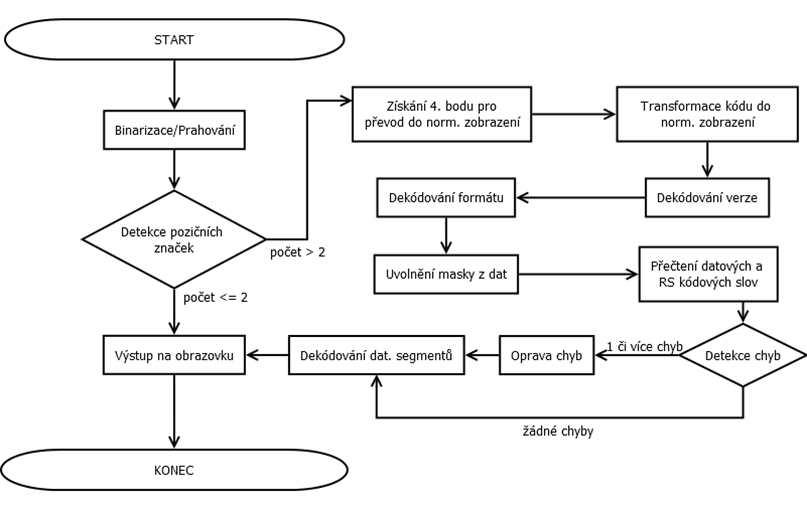
\includegraphics{fig/QRCodeReadingProcess.PNG}
    } 
    \caption{Vývojový diagram navrženého postupu pro čtení QR kódů}
    \label{QRCodeReadingProcess}
  \end{center}
\end{figure}

Kroky diagramu pro dekódování informací a opravy chyby vychází z referenčního
diagramu ISO normy (kapitola \ref{refCteniQRKodu}) a jsou doplněny o kroky
binarizace, detekce pozičních značek a transformace QR kódu z perspektivního zobrazení, jež norma
nerozvádí a zahrnuje je v jednom kroku.
Z diagramu lze vyčíst, že dekódování je proveditelné pouze tehdy, jsou-li
detekovány alespoň 3 poziční značky.

\section{Binarizace obrazu}
\label{binarizaceObrazu}

Příprava obrazu pro strojové čtení bývá často tím nejdůležitějším úkolem pro
dosažení uspokojivým výsledků. Pro čtení QR kódů lze uplatnit tzv. binarizaci
obrazu, kde se vícekanálový snímek převede na snímek ve stupni šedi, který
je poté prahován. Prahováním vzniká obraz, který obsahuje pouze dvě hodnoty,
jež představují tmavé a světlé pixely QR kódu.

Pro převod barevného obrazu na obraz ve stupních šedi se obvykle využívá
empirického vztahu barvy a intenzity

\begin{equation}
  I = 0,299R + 0,587G + 0,114B\mbox{,}
\end{equation}

\noindent kde $R$, $G$ a $B$ značí jednotlivé barevné složky.

Zvolení správné metody a parametrů pro prahování obrazu bývá již složitějším
úkolem a odvíjí se často na konkrétní doméně použití dané aplikace. Pro
prahování obrazu existují zejména dva zásadní přístupy, kdy práh je volen
globálně pro celý obraz (globální prahování) nebo lokálně (adaptivní 
prahování). Referenční algoritmus uvedený v ISO normě pracuje~s globálním
prahováním, přesto ale s ohledem na naši aplikaci, kde bude obraz pořizován z
kamery za předem neznámých světelných podmínek, můžeme tvrdit, že použití
adaptivního prahování bude výhodnější. Zvolení globální metody prahování by
mohlo vést k negativním výsledkům (obrázek
\ref{GlobalAdaptiveThresholdingComparision}) a dalo by se zvážit např. při skenování QR kódu se zdrojem světla, pokud ovšem zanedbáme možnost výskytu
přesvětlených míst.

\begin{figure}[H]
  \begin{center}
    \scalebox{0.19}{
      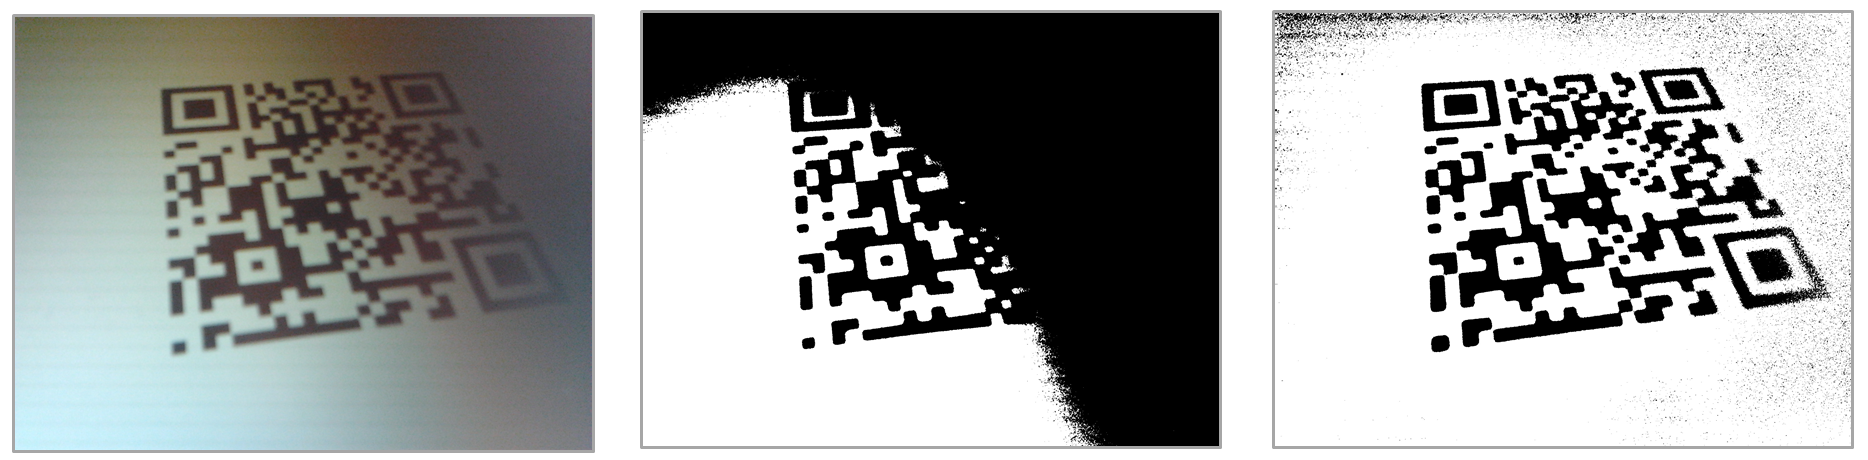
\includegraphics{fig/GlobalAdaptiveThresholdingComparision.PNG}
    }
    \caption{Porovnání globálního (uprostřed) a adaptivního prahování (vpravo)}
    \label{GlobalAdaptiveThresholdingComparision}
  \end{center}
\end{figure}

K docílení adaptivní prahování se využívá většinou přístupu Chow a Kaneko nebo
lokálního prahování. Z hlediska vysoké výpočetní složitosti prvního přístupu
pro zpracování reálného obrazu, bude v aplikaci použito lokálního prahování.
Tento přístup je založen na tvorbě matice, která se naplní vypočítanými prahy
pro každý pixel vstupního obrazu. Hodnota prahu pro daný pixel vstupního obrazu
pak může být získána jako aritmetický průměr, medián aj. jeho okolních pixelů,
kde velikost okolí je specifikována velikostí bloku prahování. V případě zvolení
malé velikosti bloku prahování může docházet v QR kódu ke tvorbě světlých míst,
adaptivní prahování zde plní spíše roli detekce hran. Naopak při zvolení velké
velikosti bloku se mohou umocňovat tmavá místa obrazu, proto je nutné volit
jeho velikost v závislosti na velikosti QR kódu. \cite{adaptiveThresholdLit}

\begin{figure}[H]
  \begin{center}
    \scalebox{0.19}{
      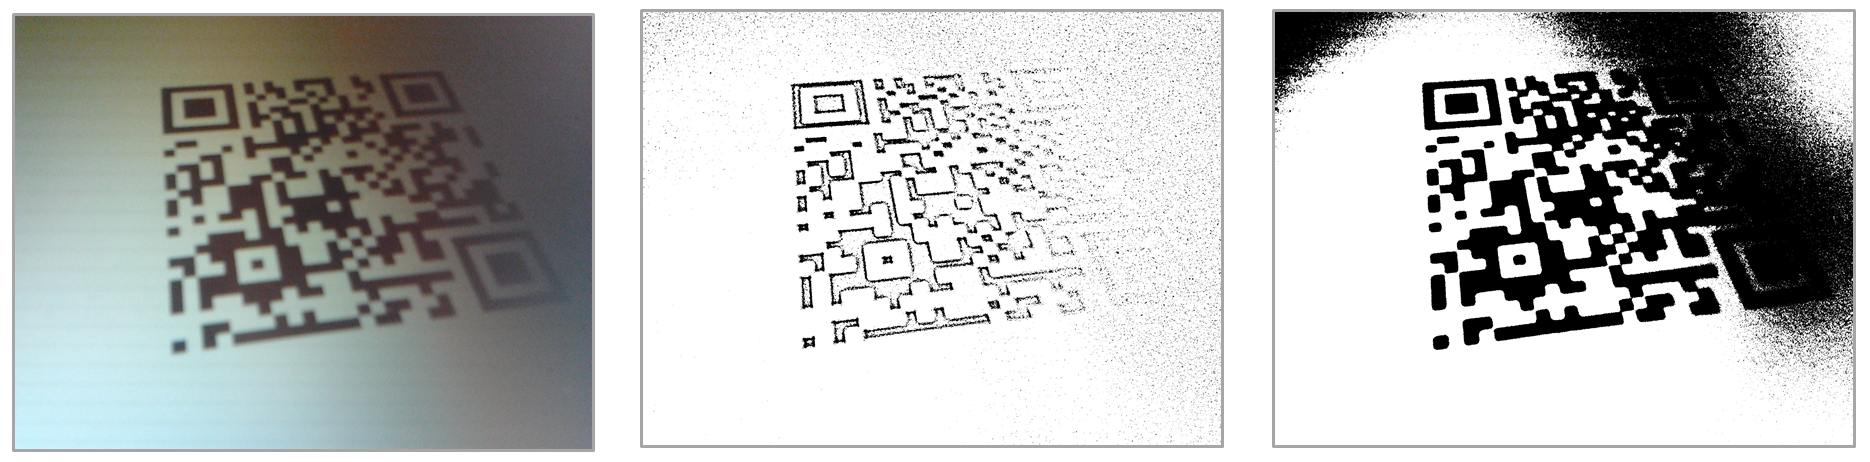
\includegraphics{fig/LocalThresholdingBadSizeOfThresholdBlock.PNG}
    }
    \caption{Výstup prahování při nevhodně zvolené velikost bloku prahování}
    \label{LocalThresholdingBadSizeOfThresholdBlock}
  \end{center}
\end{figure}

Aby byla vystihnuta vhodná závislost velikosti bloku prahování na velikosti QR
kódu, byl proveden v rámci návrhu experiment, díku kterému jsme zjistili, že
velikost bloku prahování by měla odpovídat cca jedné pětině velikosti QR kódu.
Experiment proběhl nad vzorkem obrazů o různých rozměrech, které byly tvořeny z
větší části QR kódem. Tyto vzorky byly postupně prahovány s proměnlivými
velikostmi prahovacího bloku a výsledky prahování porovnány s referenčními
obrazy. Hodnota prahu byla vypočítávána aritmetickým průměrem hodnot
okolí. Získanou závislost lze vidět na
grafu \ref{DependencyOfSizeOfThresholdBlockToQRCodeSizes}.

\begin{figure}[H]
  \begin{center}
    \scalebox{0.25}{
      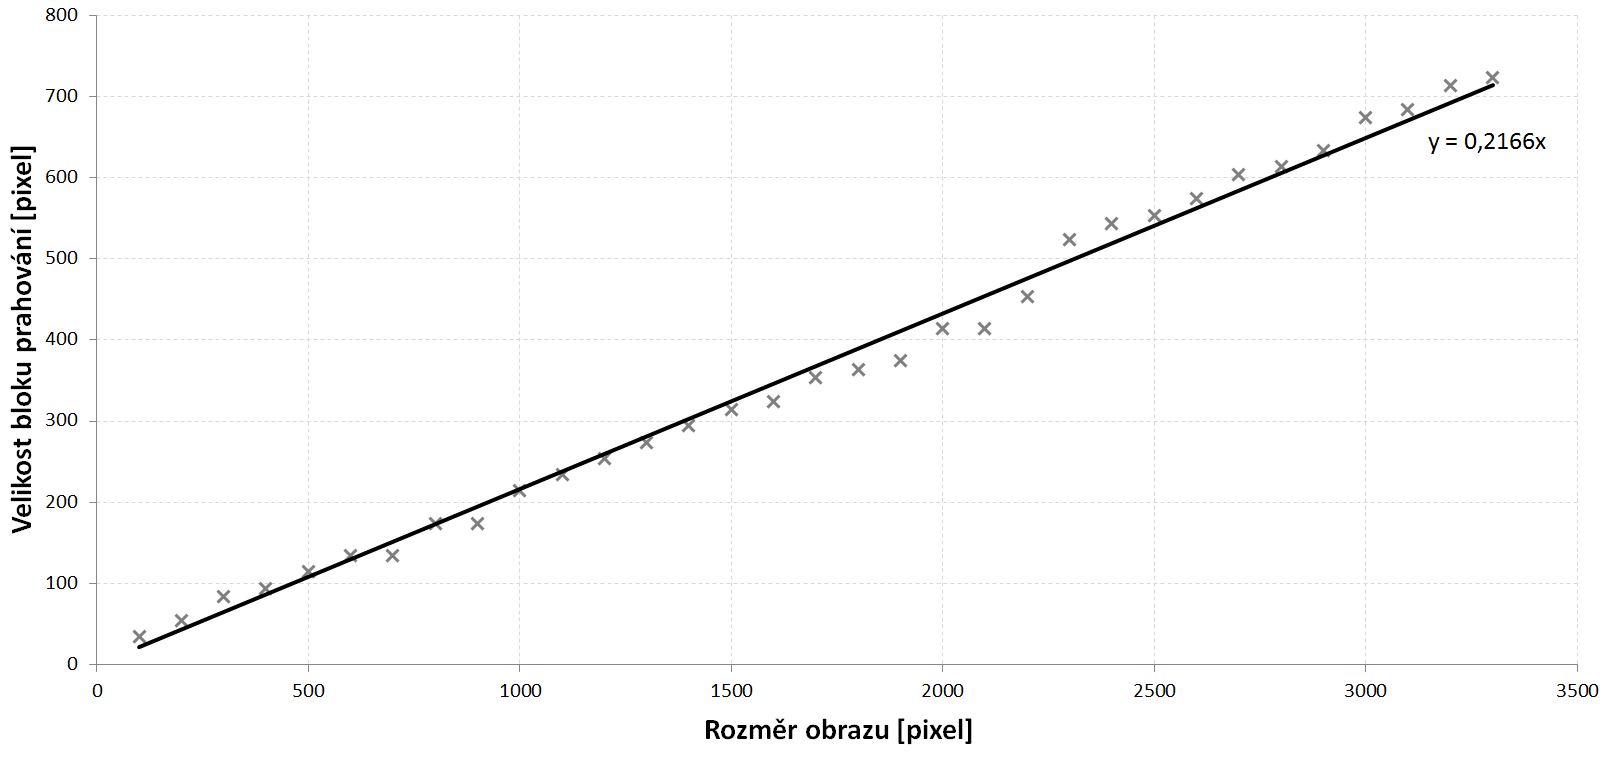
\includegraphics{fig/DependencyOfSizeOfThresholdBlockToQRCodeSizes.PNG}
    }
    \caption{Graf zavislosti vhodné velikosti bloku prahování na rozměrech QR
    kódu}
    \label{DependencyOfSizeOfThresholdBlockToQRCodeSizes}
  \end{center}
\end{figure}

Jelikož velikost QR kódu do doby jeho detekce neznáme, bude nutné v rámci
detekce QR kódu provést prahování s velikostí bloku odpovídající rozměrům
vstupního obrazu či vhodným podílům rozměrů (pro vzdálenější QR kódy). Jakmile
bude již QR kód detekován, bude známa jeho velikost, budeme moci aplikovat
prahování podle experimentálně získané referenční závislosti.

\section{Inverzní perspektivní transformace}
\label{inverzniPerspektivniTransformace}

Než se pustíme do popisu návrhu detekce a čtení QR kódu je nutno definovat pojem
a metodu inverzní perspektivní transformace, kterou budeme v následujících
kapitolách používat.

Nutnost použití inverzní perspektivní transformace se odvíjí od způsobu
interpretace QR kódu ve snímaném obraze, ve kterém je zobrazen v perspektivní
projekci, v důsledku pozice kamery v prostoru. Abychom mohli QR kód zpracovat
musíme nalézt takový vztah mezi body QR kódu a jejich odpovídajícími body v
perspektivní projekci, k čemuž slouží právě metoda homografie neboli inverzní
perspektivní transformace.

\bigskip \noindent Vztah mezi body QR kódu $(x,y)$ a body promítaného QR kódu
$(X,Y)$ lze vyjádřit jako

\begin{equation}
  p_{dst} = \mathbf{H} p_{src}\mbox{,}
\end{equation}

\begin{equation}
  \left(
    \begin{array}{c}
      x w \\
      y w \\
      w \\
    \end{array}
  \right)
  =
  \left(
    \begin{array}{ccc}
      p_{1} & p_{2}  & p_{3} \\
      p_{4} & p_{5}  & p_{6} \\
      p_{7} & p_{8}  & p_{9} \\
    \end{array}
  \right)
  \left(
    \begin{array}{c}
      X \\
      Y \\
      1 \\
    \end{array}
  \right)\mbox{,}
\end{equation}

\bigskip \noindent kde $\mathbf{H}$ je mapující maticí obsahující prvky $\vec{p}
= (p_1, \ldots, p_9)^T$, tzv. stupně svobody, platí že $|\vec{p}|=1$. 

Pro zjištění závislosti mezi body v obou zobrazeních nám stačí určit vektor
$\vec{p}$. Přičemž prvky vektoru $\vec{p}$ můžeme nalézt ze 4 kolineárních bodů
obrazu a jejich korespondujících bodů v perspektivním zobrazení a řešením 
soustavy lineárních rovnic, tak aby 
platilo $|\vec{p}|=1$ \cite{homografieCite,homografieComputerVision}: 

\begin{equation}
  \mathbf{A} \vec{p} =
  \left(
    \begin{array}{ccccccccc}
      X_{1} & Y_{1} & 1 & 0 & 0 & 0 & -X_{1} x_{1} & -Y_{1} x_{1} & x_{1} \\
      0 & 0 & 0 & X_{1} & Y_{1} & 1 & -X_{1} y_{1} & -Y_{1} y_{1} & y_{1} \\
      X_{2} & Y_{2} & 1 & 0 & 0 & 0 & -X_{2} x_{2} & -Y_{2} x_{2} & x_{2} \\
      0 & 0 & 0 & X_{2} & Y_{2} & 1 & -X_{2} y_{2} & -Y_{2} y_{2} & y_{2} \\
      X_{3} & Y_{3} & 1 & 0 & 0 & 0 & -X_{3} x_{3} & -Y_{3} x_{3} & x_{3} \\
      0 & 0 & 0 & X_{3} & Y_{3} & 1 & -X_{3} y_{3} & -Y_{3} y_{3} & y_{3} \\
      X_{4} & Y_{4} & 1 & 0 & 0 & 0 & -X_{4} x_{4} & -Y_{4} x_{4} & x_{4} \\
      0 & 0 & 0 & X_{4} & Y_{4} & 1 & -X_{4} y_{4} & -Y_{4} y_{4} & y_{4} \\
    \end{array}
  \right)
  \left(
    \begin{array}{c}
      p_{1} \\
      p_{2} \\
      p_{3} \\
      p_{4} \\
      p_{5} \\
      p_{6} \\
      p_{7} \\
      p_{8} \\
      p_{9} \\
    \end{array}
  \right)
  = 0\mbox{.}
\end{equation}

\section{Detekce pozičních značek}
\label{detekcePozicnichZnacek}

Pro detekci pozičních značek norma zmiňuje použití skenovací linie, tato metoda
je velmi efektivní a výhodná pro použití v reálném obraze. Ve svém principu 
využívá poměrů mezi tmavými a světlými moduly pozičních značek a je velmi dobře
uplatnitelná u obrazů, ve kterých není QR kód v perspektivní projekci. K
docílení čtení QR kódů i při velmi extrémním perspektivním zkreslení, kdy poměry
mezi tmavými a světlými moduly pozičních značek jsou znehodnoceny, budeme
detekci provádět pomocí hledání kontur (kapitola \ref{hledaniKontur}). Základní
navržený princip vycházející z normy pomocí skenovací linie si přesto popíšeme
v~kapitole \ref{skenovaciLinie}.

\subsection{Skenovací linie}
\label{skenovaciLinie}

Princip hledání pozičních značek s využitím skenovací linie, lze definovat
procházením jednotlivých řádků obrazu a hledáním takové sekvence tmavých a
světlých bodů, která by odpovídala poměru 1:1:3:1:1. Akceptovaná nepřesnost v
poměru je dána podle normy hodnotou 0.5, takže lze např. přijmout i sekvenci v
poměru 0.5:1.5:2.5:0.5:1.5. Jakmile tuto sekvenci bodů skenovací linie nalezne
(obrázek \ref{QRCodeDetectionWithScanline}), dojde k jejímu rozšíření ve
vertikálním směru nahoru i dolů, dokud není dosaženo hranice vnitřního tmavého čtverce poziční značky. Střed poziční
značky poté můžeme zjistit z průsečíků středových linií. První středová linie je
zkonstruována ze středů úseček, ležících na rozšířených skenovacích liniích,
definovaných hranicemi poziční značky. Ke zjištění druhé středové linie musíme
využít skenovací linie ve vertikálním směru a obdobného postupu.

\begin{figure}[H]
  \begin{center}
    \scalebox{0.18}{
      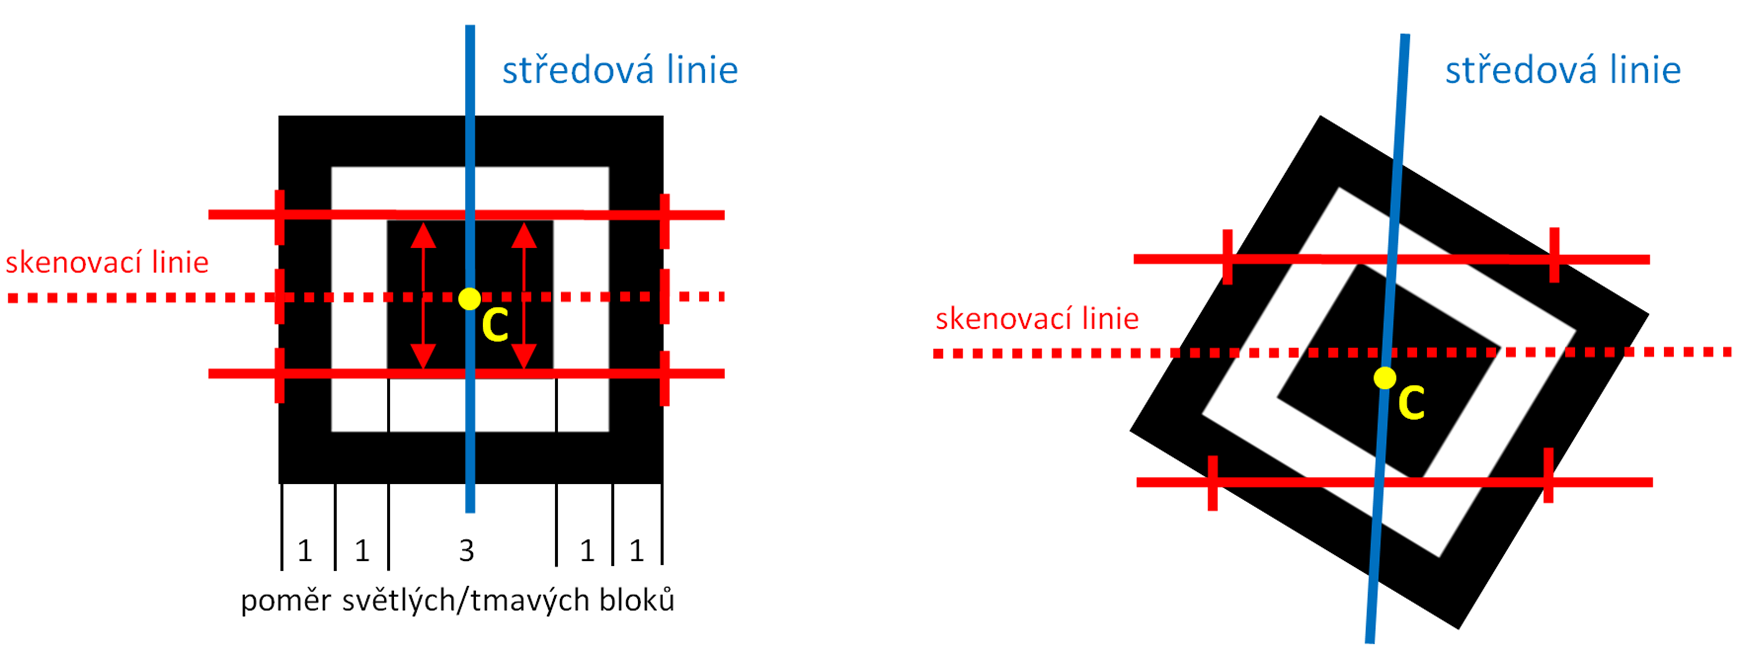
\includegraphics{fig/QRCodeDetectionWithScanline.PNG}
    }
    \caption{Detekce poziční značky pomocí skenovací linky}
    \label{QRCodeDetectionWithScanline}
  \end{center}
\end{figure}

\subsection{Hledání kontur}
\label{hledaniKontur}

Hledání kontur slouží ke strukturální analýze obrazu. Algoritmy na hledání
kontur pracují většinou s již binarizovanými obrazy a jejich princip spočívá ve
hledání spojených komponent buď 1 pixely (tzv. 1-komponenty) nebo 0 pixely 
(tzv. 0-komponenty či díry). Nejpoužívanějšími algoritmy jsou Square tracing,
Moore-Neighbor, Radial Sweep aj. Vyjma těchto algoritmů existují i algoritmy,
které dokáží rozpoznat a uchovat topologii mezi nalezenými strukturami, jedním
z nich je např. Suzuki 85 algoritmus \cite{suzukiLit}.

\begin{figure}[H]
  \begin{center}
    \scalebox{0.23}{
      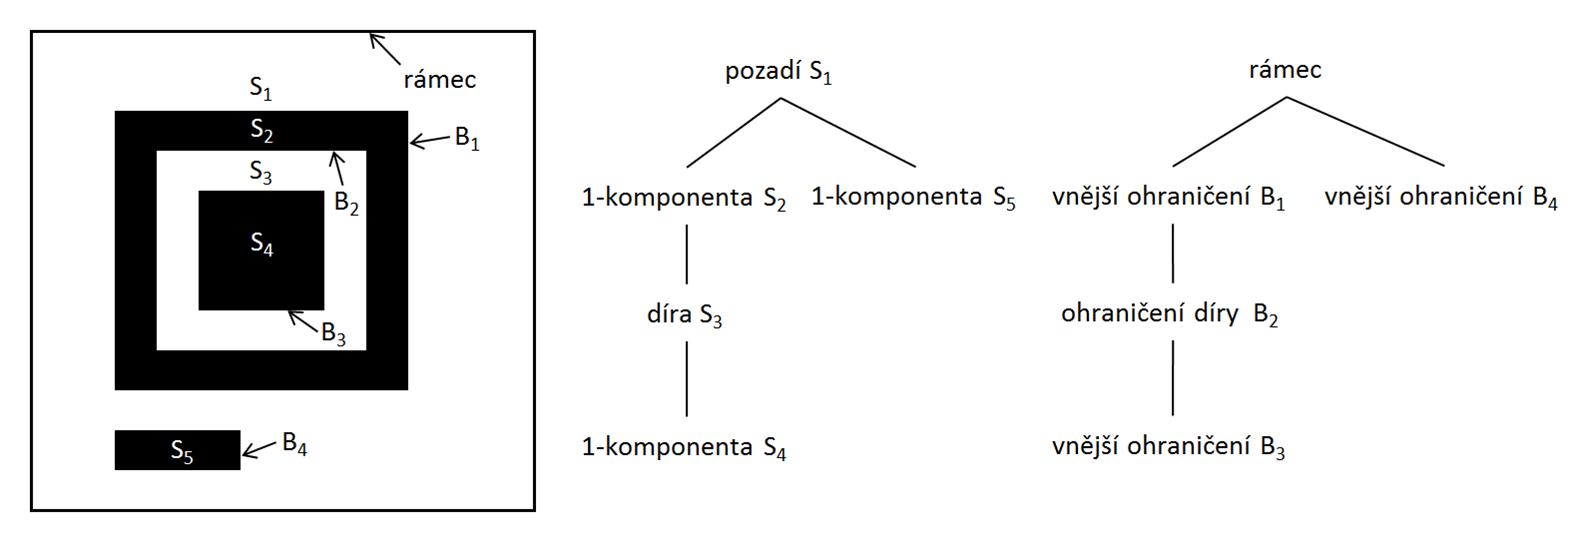
\includegraphics{fig/ContourTopology.PNG}
    }
    \caption{Výstup nálezu kontur a sestavení topologické závislosti mezi nimi}
    \label{ContourTopology}
  \end{center}
\end{figure}

Využití topologie by mohlo vést ke zrychlení detekce pozičních značek, neboť
víme, že poziční značka musí být tvořena právě jednou další 1-komponentou
(obrázek \ref{ContourTopology}), čehož lze využít k rychlému zahazování
neplatných struktur. Topologie by šla využít i pro detekci a zpracování více QR
kódů v obraze, kde by ovšem musel být každý QR kód ohraničen tzn. být ve vlastní struktuře. Identifikace a přiřazení
pozičních značek k jednotlivým QR kódům by poté probíhalo na základě shodnosti
rodičovské struktury. Právě z těchto důvodů bude v implementaci využito
topologické analýzy a Suzuki algoritmu.

Výsledkem hledání kontury bývá vždy množina bodu, která sleduje danou strukturu,
v našem případě např. poziční značku. Pokud uvážíme již i nějaký druh
interpolace bodů, možný výsledek detekce poziční značky by mohl vypadat tak,
jak je znázorněno na obrázku \ref{FinderMarkContourDetection}:

\begin{figure}[H]
  \begin{center}
    \scalebox{0.17}{
      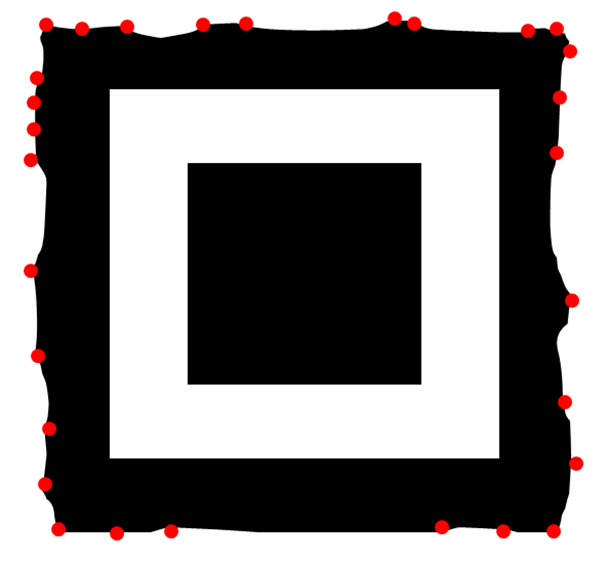
\includegraphics{fig/FinderMarkContourDetection.PNG}
    }
    \caption{Předpokládaný interpolovaný výstup bodů hledání kontury pro
    poziční značku}
    \label{FinderMarkContourDetection}
  \end{center}
\end{figure}

Poziční značka, jako obrazec čtvercovitého charakteru, je přesně definována
čtyřmi body (rohy). Množina bodů kontury nám ovšem tuto informaci přímo nedává,
ba dokonce rohy v kontuře mohou být různě zdeformované, proto je nutno skutečné,
resp. pomyslné rohy poziční značky zjistit jiným způsobem. Pro tento účel byl
navržen algoritmus hledání rohů polygonu, jehož přesné znění lze nalézt v
příloze \ref{algoritmusHledaniRohu} a vizualizaci jeho činnosti na následujícím
obrázku \ref{SearchCornersOfPolygonAlgorithm}.

\begin{figure}[H]
  \begin{center}
    \scalebox{0.25}{
      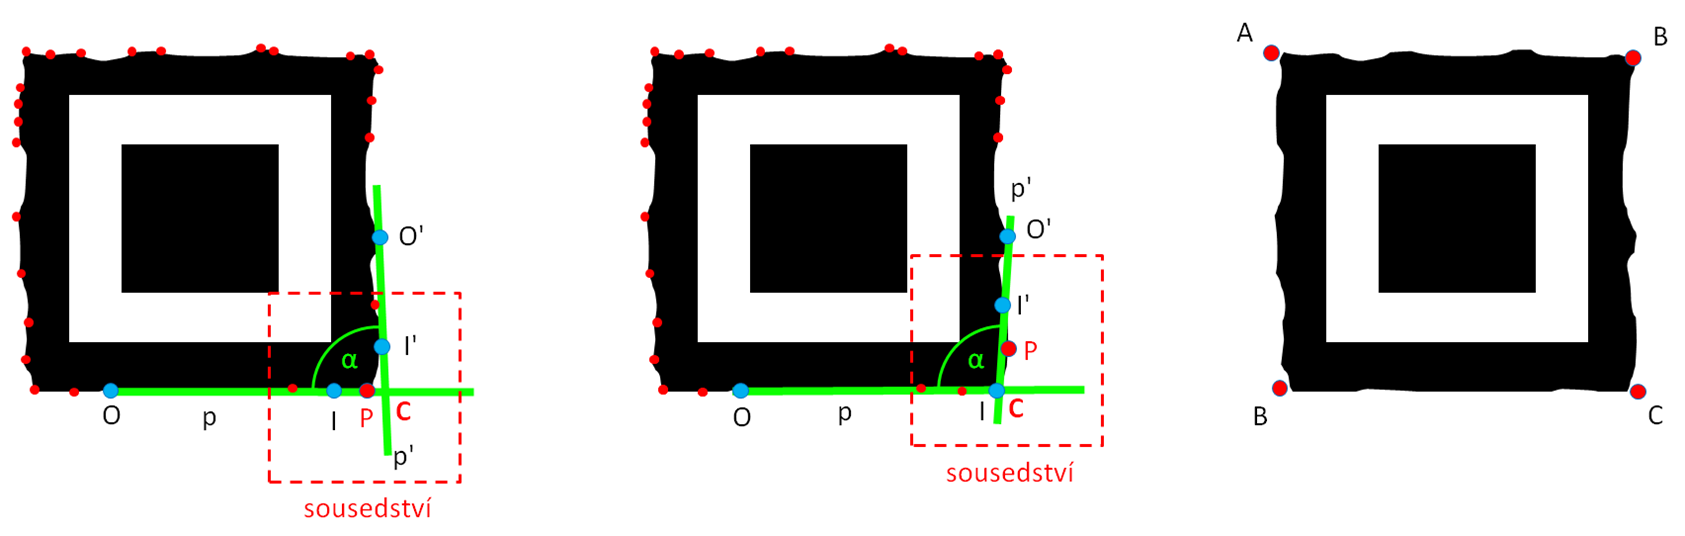
\includegraphics{fig/SearchCornersOfPolygonAlgorithm.PNG}
    }
    \caption{Výstup algoritmu hledání rohů polygonu (zde poziční značky)}
    \label{SearchCornersOfPolygonAlgorithm}
  \end{center}
\end{figure}

Pokud algoritmus hledání rohů polygonu skončí se čtyřmi nalezenými rohy, můžeme
se domnívat, že se jedná o poziční značku a provést další potřebné kroky k 
jejímu ověření, v opačném případě lze danou strukturu zahodit a přejít na
zpracování další struktury. Při nálezu čtyř rohů přistoupíme k inverzní
perspektivní transformaci dané struktury na základě těchto bodů do
normalizovaného zobrazení. Šablonovým porovnáním poté zjistíme, zda se
jedná o poziční značku či ne a přejdeme na zpracování další struktury. Výsledný
vývojový diagram celého procesu detekce lze vidět na následujícím obrázku
\ref{QRCodeDetectionProcess}.

\begin{figure}[H]
  \begin{center}
    \scalebox{0.20}{
      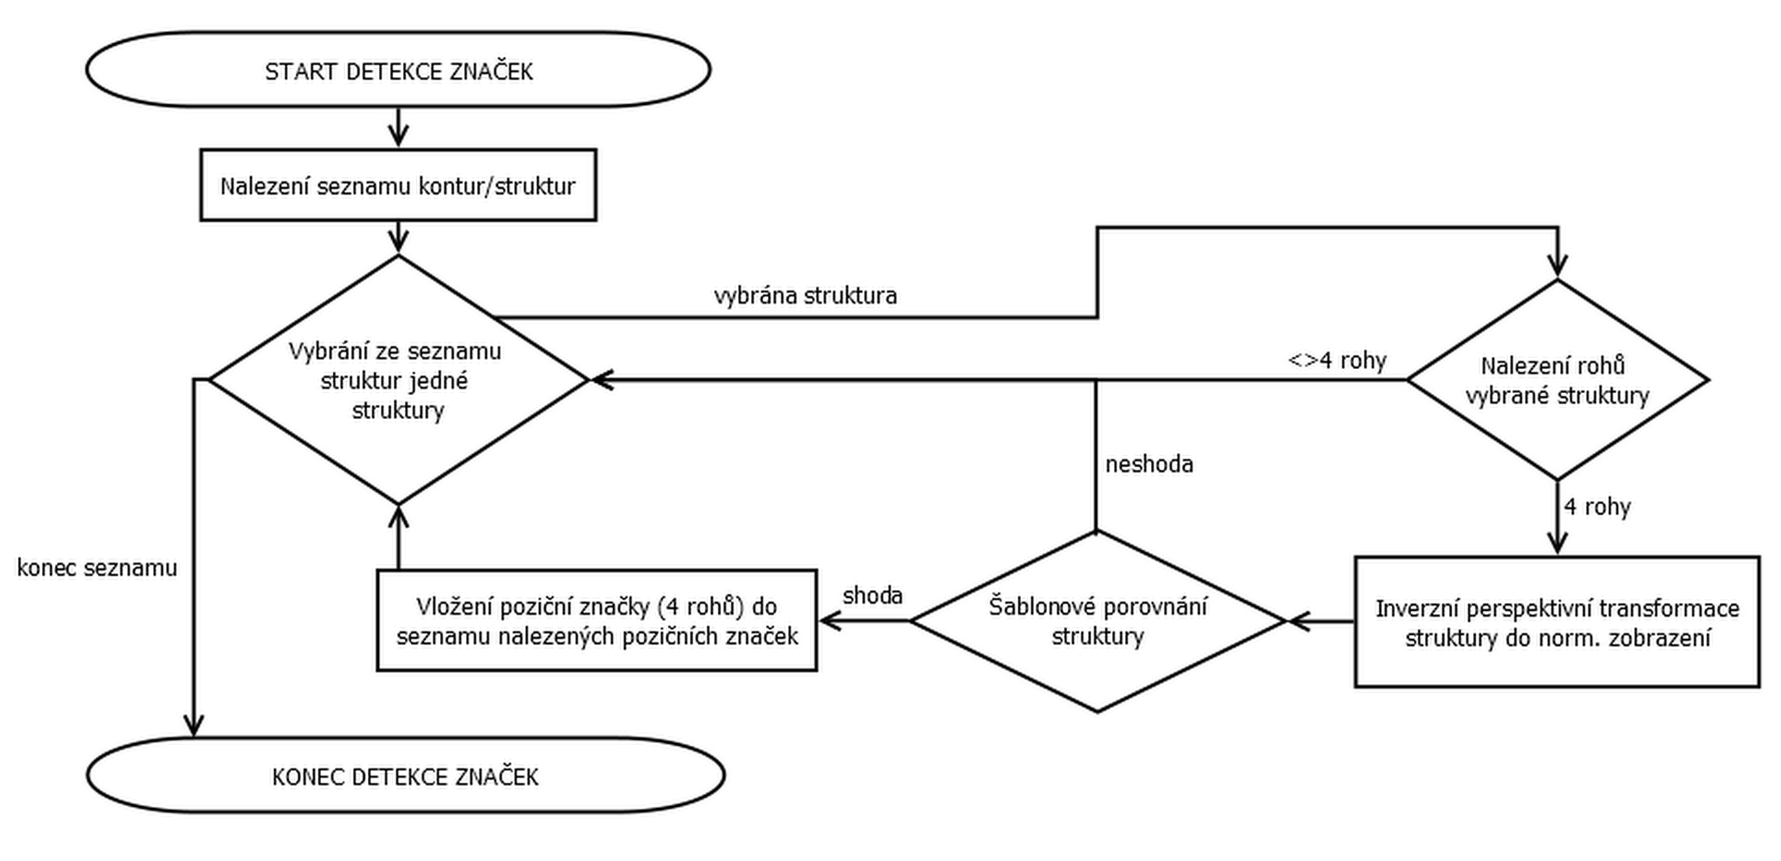
\includegraphics{fig/QRCodeDetectionProcess.PNG}
    } 
    \caption{Proces detekce pozičních značek QR kódu}
    \label{QRCodeDetectionProcess}
  \end{center}
\end{figure}

\section{Zjištění a transformace oblasti QR kódu}
\label{zjisteniATransformace}

Proces detekce pozičních značek nám bude vracet seznam dekovaných značek, kde
každá značka bude přesně definována čtyřmi body seřazenými ve směru hodinových
ručiček. Abychom mohli takto detekovaných značek využít pro převod QR kódu do
normalizovaného zobrazení, budeme muset nejprve poziční značky a jejich body
uspořádat a identifikovat jejich umístění v QR kódu. Jelikož se poziční značky
nachází v QR kódu pouze tři, ve třech rozích, a pro inverzní perspektivní
transformaci je zapotřebí čtyř bodů, budeme muset určit i tento čtvrtý bod
(roh QR kódu).

Postup seřazení pozičních značek (obrázek \ref{QRCodeArea}) by mohl být založen
na vytvoření pomyslného trojúhelníku ze středů pozičních značek, výpočtu jeho těžiště, díky
němuž by šlo poziční značky uspořádat ve směru hodinových ručiček. Tímto
seřazením by nám stále ale scházela informace o pozici značek a jejich bodů 
v rámci QR kódu, tuto informaci by šlo získat na základě nalezení bodů
pozičních značek $X$, $Y$, $Z$, které se nachází uvnitř QR kódu. Vnitřní bod
každé poziční značky by byl nalezen otestováním všech bodů dané poziční značky a
zjištěním takového bodu, který je nejvzdálenějším bodem ke vnitřní stěně našeho
pomyslného trojúhelníku nebo nejbližším bodem ke vnější straně trojúhelníku,
neexistuje-li žádný bod poziční značky uvnitř trojúhelníku. Poté můžeme tvrdit,
že levá horní poziční značka je taková značka, jež obsahuje nejvzdálenější
vnitřní bod $Y$ poziční značky od vnitřní strany pomyslného trojúhelníku.

\begin{figure}[H]
  \begin{center}
    \scalebox{0.17}{
      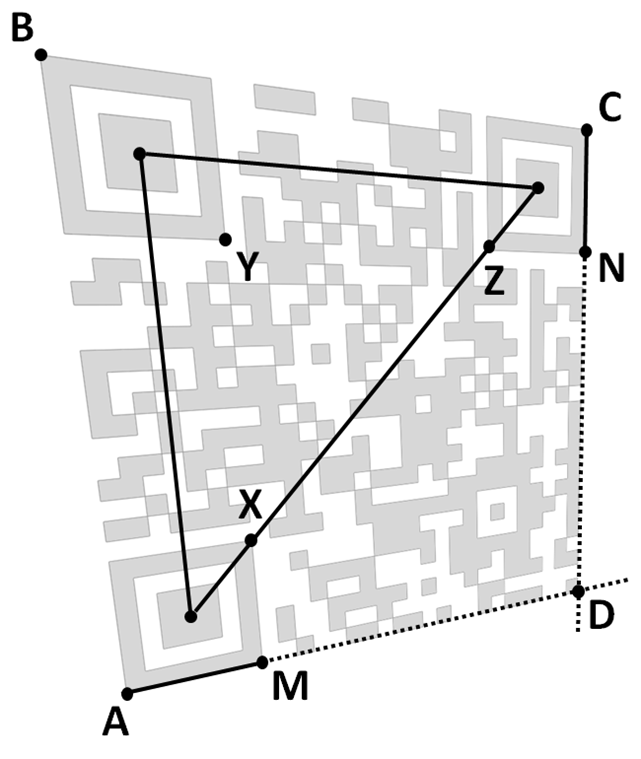
\includegraphics{fig/QRCodeArea.PNG}
    } 
    \caption{Znázornění postupu zjištění čtyř bodů pro inverzní perspektivní
    transformaci}
    \label{QRCodeArea}
  \end{center}
\end{figure}

Po seřazení bodů pozičních značek již budeme moci určit i čtyři body pro
inverzní perspektivní transformaci $A$, $B$, $C$ a $D$, kde poslední bod $D$
potřebný pro transformaci by bylo možné v případě ideálně sejmutého QR kódu získat protnutím
polopřímek $AM$ a $CN$. V praxi se ovšem můžeme setkat i s nepřesně detekovanými
pozičními značkami, proto byly navrženy další dva postupy získání 4. bodu (rohu)
QR kódu (obrázek \ref{DeterminingTheFourthPointForTransformation}).	

\begin{figure}[H]
  \begin{center}
    \scalebox{0.23}{
      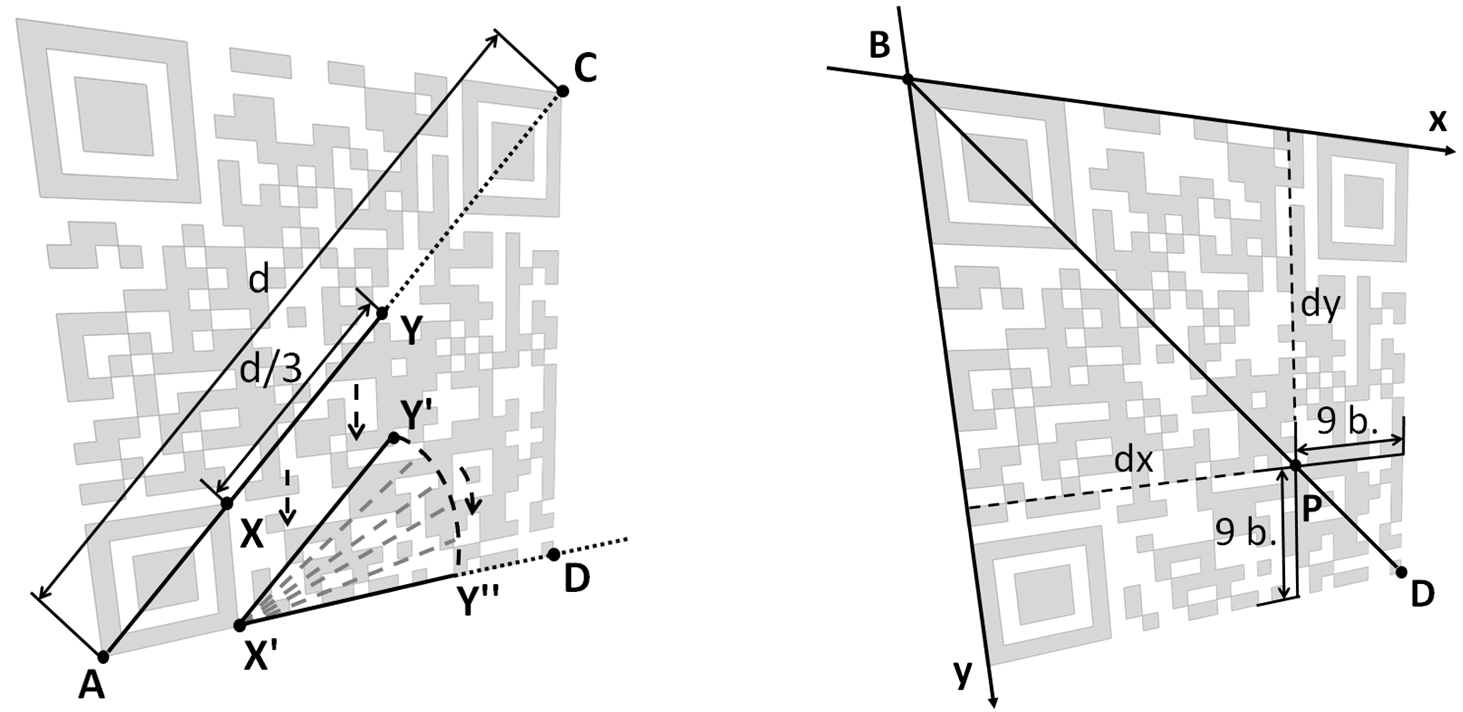
\includegraphics{fig/DeterminingTheFourthPointForTransformation.PNG}
    } 
    \caption{Zjištění 4. bodu vzorkováním (vlevo) a pomocí zarovnávací značky
    (vpravo)}
    \label{DeterminingTheFourthPointForTransformation}
  \end{center}
\end{figure}

První navržený postup hledání 4. bodu je založen na konstrukci vzorkovací úsečky
(obdélníku) $X'Y'$, která vzorkuje QR kód postupnou rotací z počátečního bodu 
$X'$ ve směru hodinových ručiček, dokud není dosaženo světlého pozadí, které
kód obklopuje. Po skončení vzorkování můžeme rozšířením vzorkovací úsečky 
$X'Y''$ získat polopřímku, na které bude ležet bod $D$. Pokud totéž provedeme i
vůči pravé horní poziční značce a proti směru hodinových ručiček, tak bod $D$
získáme právě z průsečíku námi rozšířených vzorkovacích úseček.

Druhý postup hledání 4. bodu není použitelný pro QR kódy verze 1, které
neobsahují zarovnávací značky. Principiálně ke své činnosti využívá jiné 
z předešlých metod pro převod do dočasného normalizovaného zobrazení, ve
kterém nalezne pozici bodu $D$ pomocí pravé dolní zarovnávací značky a poté
opět zpětně tento bod transformuje do perspektivního zobrazení.

K nalezení skutečné pozice $P$ zarovnávací značky v normalizovaném zobrazení
využijeme šablonového vyhledávání, abychom ale mohli vytvořit šablonu, musíme
nejprve vhodně zjistit velikost jednoho modulu. Pro výpočet pozice bodu $D$ bude
nutno také zjistit referenční pozici $s$ zarovnávací značky (viz ISO norma
tabulka E.1), což zahrnuje i přečtení verze QR kódu. Při znalosti, že bod $D$
je od zarovnávací značky vždy vzdálen 9 bodů oběma směry, platí:

\begin{equation}
  D = \bigg[ B_{x} + \frac{dx}{s}(s + 9) ; B_{y} + \frac{dy}{s}(s + 9)
  \bigg]\mbox{,}
\end{equation}

\begin{equation}
  dx = P_{x} - B_{x}\mbox{,} \quad dy = P_{y} - B_{y}\mbox{.}
\end{equation}

Po získání bodu $D$ v normalizovaném zobrazení stačí již pouze tento bod převést
zpátky do perspektivního zobrazení. Tento postup hledání 4. bodu byl navržen 
z důvodu umožnění čtení QR kódů na znečištěném podkladu, což by vedlo k selhání
první uvedené metody.

\section{Čtení QR kódu}
\label{cteniQRKodu}

Pro čtení QR kódu bude implementována čtecí mřížka (obrázek \ref{SamplingGrid}),
která bude na celý QR kód přikládána. Jednotlivé moduly  QR kódu reprezentující bity budou
vzorkovány ze středu každé buňky přiložené mřížky. Vzorkovaná oblast bude zabírat
3x3 pixely, tak je uvedeno v referenčním algoritmu ISO normy.

\begin{figure}[H]
  \begin{center}
    \scalebox{0.20}{
      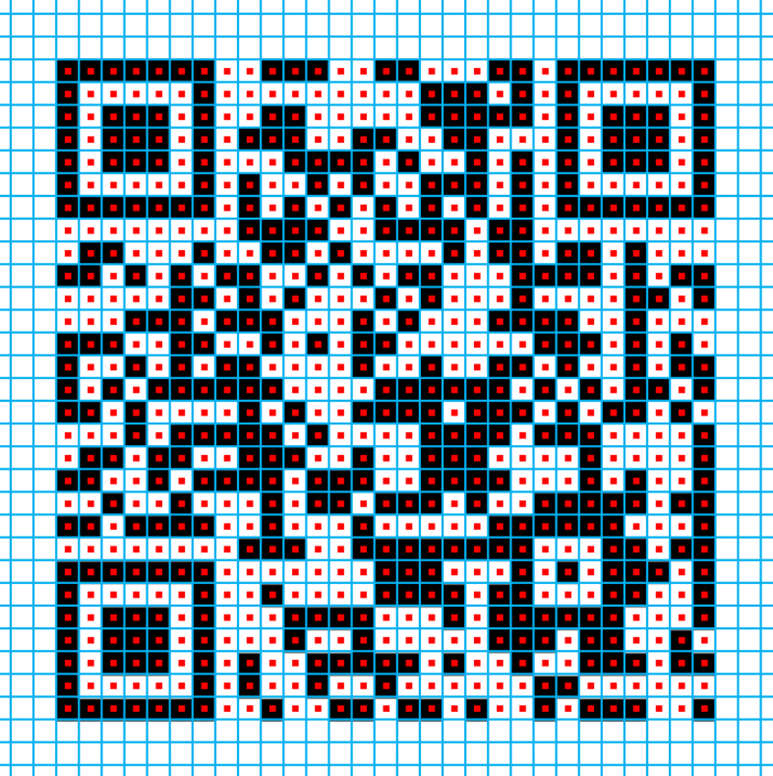
\includegraphics{fig/SamplingGrid.PNG}
    } 
    \caption{Ustanovení vzorkovací mřížky a oblastí vzorkování (červená barva)}
    \label{SamplingGrid}
  \end{center}
\end{figure}

O počtu řádků a sloupců mřížky bude rozhodnuto v závislosti na detekované verzi
$V$ QR kódu (obrázek \ref{DeterminingTheVersionOfQRCode}), která bude zprvu určena
vtahem (dle ISO normy)

\begin{equation}
  V = \frac{7 D}{2 (W_{UL} + W_{UR})} - 2,5\mbox{.}
\end{equation}

\begin{figure}[H]
  \begin{center}
    \scalebox{0.13}{
      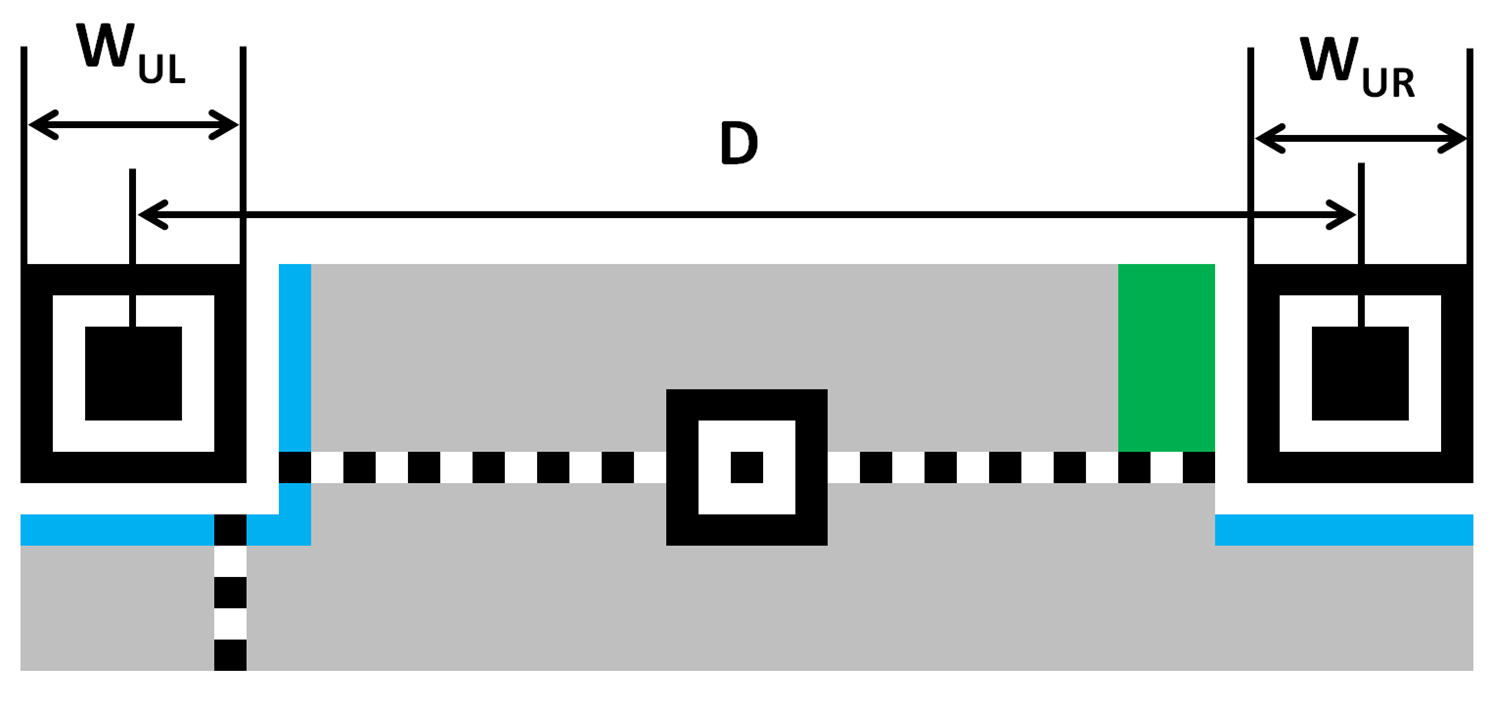
\includegraphics{fig/DeterminingTheVersionOfQRCode.PNG}
    } 
    \caption{Zjištění dočasné verze QR kódu podle jeho rozměrů}
    \label{DeterminingTheVersionOfQRCode}
  \end{center}
\end{figure}

Bude-li detekován QR kód verze 6 nebo nižší, bude tato verze považována jako
finální. V opačném případě dojde k upřesnění verze $V$ přečtením metainformace 
o verzi z QR kódu. 

\section{Architektura cílové aplikace}
\label{architekturaCiloveAplikace}

Aplikace čtečky bude implementována pro platformu Android s ohledem na případné
znovuvyužití stěžejních algoritmů zajišťujících čtení QR kódu i na ostatních
mobilních platformách. Nejenom z tohoto důvodu, ale také i z efektivního využití
výpočetních prostředků, bude implementována detekce a čtení QR kódu v nativním
kódu jazyka C++. Sestavené C++ moduly budou poté ve formě sdílené knihovny
(\texttt{Barcodes Library}) linkovány do naší aplikace, ve které bude nutno
implementovat rozhraní pro komunikaci s naší knihovnou z~jazyka Java
(\texttt{JNI Library}) (obrázek \ref{QRReaderApplicationLibraryDependency}).

\begin{figure}[H]
  \begin{center}
    \scalebox{0.20}{
      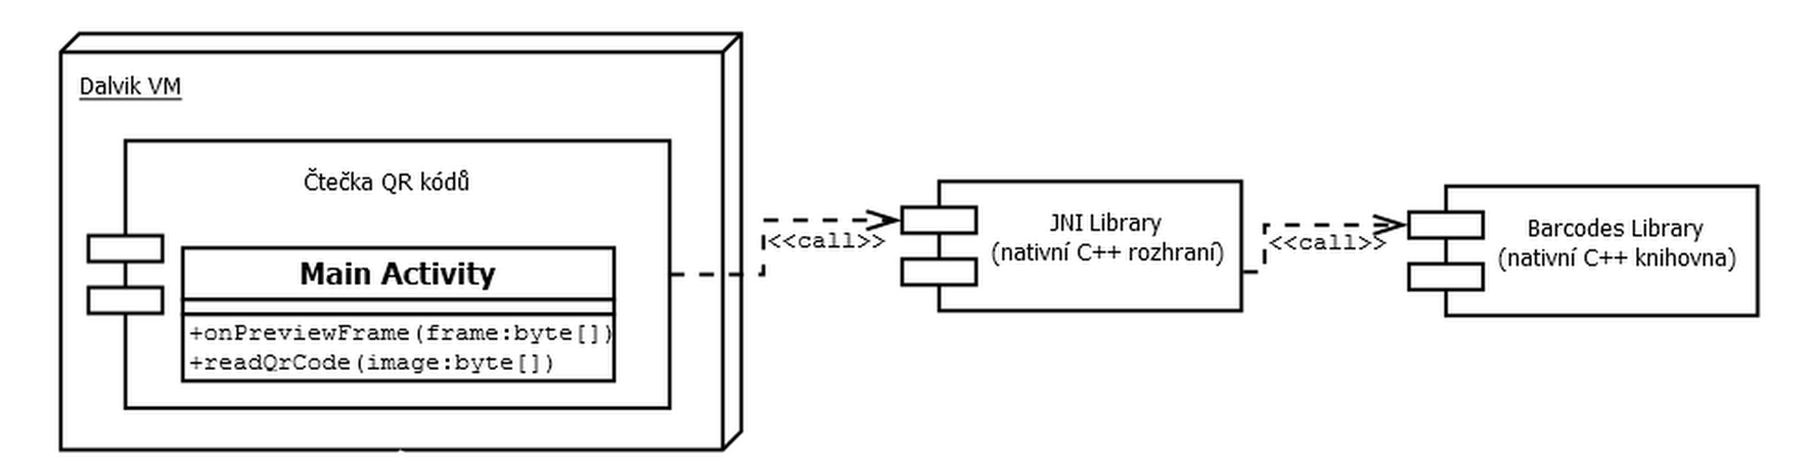
\includegraphics{fig/QRReaderApplicationLibraryDependency.PNG}
    } 
    \caption{Knihovní závislosti aplikace čtečky QR kódů}
    \label{QRReaderApplicationLibraryDependency}
  \end{center}
\end{figure}

Z důvodu snadné rozšiřitelnosti aplikace o nově čitelné QR kódy, bez potřeby
překládání nativní knihovny, bude knihovna \texttt{Barcodes Library} obsahovat
pouze dekodér fyzické vrstvy, který je pro všechny případy použití QR kódu
neměnný. Dekodér aplikační vrstvy bude implementován až v rámci aplikace a jazyce Java. Jelikož nám Dalvik
dovoluje dynamické načítání tříd pomocí \texttt{DexClassLoader}, bude zvážena i
možnost instalování dekodérů aplikační vrstvy za běhu aplikace ve formě zásuvných modulů.

Rozhraní mezi nativní knihovnou a aplikací bude obsahovat řadu obalujících
objektů, které budou zprostředkovávat převod C++ objektů na Java objekty a 
naopak. Aplikací budou volány z rozhraní pouze dvě funkce, jedna pro detekci
QR kódu v reálném obraze a druhá pro dekódování QR kódu ze sejmutého obrazu
(obrázek \ref{QRReaderApplicationNativeCalls}).

\begin{figure}[H]
  \begin{center}
    \scalebox{0.55}{
      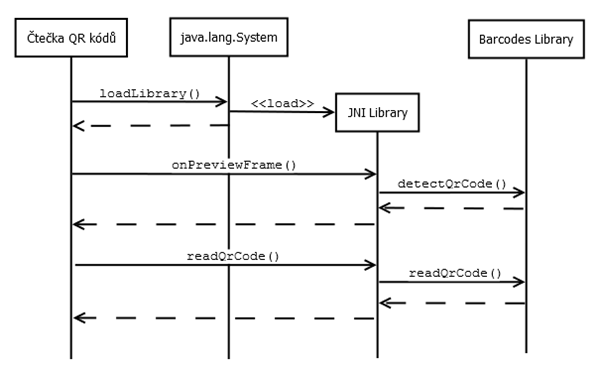
\includegraphics{fig/QRReaderApplicationNativeCalls.PNG}
    } 
    \caption{Sekvenční diagram znázorňující volání funkcí nativního rozhraní}
    \label{QRReaderApplicationNativeCalls}
  \end{center}
\end{figure}

\chapter{Implementace}
\label{implementace}

Následující kapitola pojednává o samotné realizaci navržených algoritmů a 
aplikaci čtečky QR kódů v kapitole \ref{navrh}. Popis implementace je zaměřen na
uvedení nejzákladnějších tříd, metod či funkcí, které implementují nejdůležitější části
výsledné aplikace, přičemž podrobný popis lze nalézt v programových 
dokumentacích na přiloženém DVD (příloha \ref{obsahDVD}).

\section{Knihovna pro čtení QR kódů}
\label{knihovnaBarcodesLibrary}

Knihovna pro rozpoznání QR kódů (kapitola \ref{detekceQrKoduBarcodesLibr}),
čtení a dekódování jejich fyzické vrstvy (kapitola
\ref{cteniQrKoduBarcodesLibr}) byla implementována v jazyce C++.
Při práci s obrazem bylo využito open source knihovny OpenCV. Strukturálně byla
knihovna realizována tak, aby ji bylo možné v budoucnu případně rozšířit o
nově podporované čárové kódy.

\subsection{Detekce QR kódu}
\label{detekceQrKoduBarcodesLibr}

K detekci QR kódu v obraze slouží singleton třída \texttt{QrDetector} a její
metoda \texttt{detect()}, jejíž parametry jsou:

\begin{itemize}
  \item \texttt{image} -- vstupní zpracovávaný obraz, který je již reprezentován
  ve stupních šedi;
  \item \texttt{detectedMarks} -- výstup vektor s detekovanými rohy pozičních
  značek QR kódu v~obraze;
  \item \texttt{flags} -- doplňující informace pro detekci ve formě bitových
  vlajek.
\end{itemize}

Výsledek činnosti metody detekce velmi předurčuje právě poslední parametr
\texttt{flags}, jenž slouží zejména pro specifikaci předpokládané vzdálenosti QR
kódu v obraze. Zadaná vzdálenost QR kódu ovlivňuje výpočet velikosti bloku
prahování, tzn. výsledný binarizovaný obraz, kde budou detekovány poziční značky.

Byly zvoleny celkem čtyři předpokládané vzdálenosti QR kódu, které mohou být
předány metodě i současně. Jedna ze vzdáleností odpovídá velmi blízkému QR kódu
a pokud je předána, tak se pro výpočet velikosti bloku prahování uplatní
experimentálně zjištěná referenční závislost (obrázek
\ref{DependencyOfSizeOfThresholdBlockToQRCodeSizes} v kapitole \ref{binarizaceObrazu}).
Ostatní tři vzdálenosti jsou určeny pro vzdálenější QR kódy, konkrétně pro QR kódy 
o velikosti $1/3$, $1/6$ a $1/12$ celkového obrazu. Velikost bloku prahování v
tomto případě je dána stejnou poměrnou částí referenční závislosti.

Pokud předáme metodě více předpokládaných vzdáleností QR kódu, budou algoritmem
detekce preferovány nejprve ty menší, neboť lze předpokládat, že QR kód budeme
číst většinou z blízké vzdálenosti. Nenalezne-li algoritmus alespoň tři poziční
značky v nejmenší předané vzdálenosti, zkusí vybrat další větší předpokládanou
vzdálenost QR kódu. Tento proces algoritmus opakuje, dokud nejsou vybrány
všechny předpokládané vzdálenosti z~\texttt{flags} nebo nejsou nalezeny alespoň
tři poziční značky. Jelikož během detekce, která běží v~několika krocích, může
dojít k detekci stejných značek, bylo nutné implementovat i mechanismus filtrování
těchto značek.

\bigskip \noindent Proces detekce byl implementován podle navrženého postupu:

\begin{enumerate}
  \item \textbf{Nalezení všech struktur} v obraze pomocí hledání kontur Suzuki
  85 algoritmem a funkcí \texttt{findContours()}, kterou již implementuje
  knihovna OpenCV.
  \item \textbf{Zjištění rohů struktur} metodou
  \texttt{Polygon2D::findCorners()} (příloha \ref{algoritmusHledaniRohu}) a zahození struktur,
  pokud u nich nebyly nalezeny přesně 4 rohy.
  \item \textbf{Převedení obrazu} do normalizovaného zobrazení funkcí
  \texttt{warpPerspective()}.
  \item \textbf{Šablonové porovnání} struktury s šablonou poziční značky funkcí
  \texttt{exactMatch()}.
\end{enumerate}

\subsection{Optimalizace detekce pozičních značek}
\label{optimalizaceDetekce}

Z důvodu urychlení detekce pozičních značek, tzn. vyhnutí se časově drahému převodu obrazu z perspektivního zobrazení do normalizovaného, byly přidány s využitím OpenCV do již implementovaného algoritmu detekce další tři kroky. Svojí funkcí plní jakési filtry, které mají za úkol zahazovat struktury, jež nejsou s velkou pravděpodobností pozičními značkami.

\textbf{První filtr} je založen na nalezení nejmenšího ohraničujícího obdélníku
(obrázek \ref{MinimalBoundedAndConvexHull}) dané struktury. Filtr slouží pro
zahazování segmentů, jejichž ohraničující obdélník má příliš malé rozměry nebo je velký poměrový rozdíl
velikostí šířky a délky tohoto obdélníku. V~ideálním případě poziční značky
je poměr mezi šířkou a délkou 1:1. Jelikož poziční značka může být
perspektivně zkreslena, byl zvolen jako maximální přípustný poměr 1:4.
 
 \begin{figure}[H]
  \begin{center}
    \scalebox{0.18}{
      
\includegraphics{fig/minimalBoundedConvexxHull.PNG}
    }
    \caption{Nejmenší ohraničující obdélník (vlevo) a konvexní obálka (vpravo)
    struktury}
    \label{MinimalBoundedAndConvexHull}
  \end{center}
\end{figure}

\textbf{Druhý filtr}, který byl zařazen do algoritmu, provádí analýzu poměru
tmavých a bílých pixelů struktury. V~ideálním případě struktury poziční značky
je tento poměr 49:16. V~rámci detekce ale tolerujeme až neshodu v 8 bodech,
tudíž akceptujeme i poměry 57:8 či 41:24.

\textbf{Třetí filtr} vytvoří kolem detekované struktury konvexní obálku (obrázek
\ref{MinimalBoundedAndConvexHull}) a zjistí počet pixelů uvnitř této obálky. S
využitím předchozího filtru, kde jsme získali počet pixelů struktury, můžeme obě hodnoty porovnat. Jelikož tvar
poziční značky je přesně určen pouze svými 4 nekolineárními body a součet
vnitřních úhlů je 360°, nikdy nemůže u struktury ideální poziční značky nastat,
že by některý z vnitřních úhlů byl konkávní. Konkávnost vnitřních úhlů je možné
získat až pro 5 a více bodů. I když počet bodů konvexní obálky a struktury
poziční značky by měl být totožný, implementačně je tolerována až 10\% neshoda.

Pokud budeme prezentovat funkci filtrů na ukázkovém obrazu (obrázek
\ref{SevenThousandsStructures}), jenž obsahuje celkem 7000 nalezených struktur, filtry připustí k otestování na
poziční značku pouze 21 z nich. Většina struktur je odstraněna již v prvním
filtru, konkrétně 6742. Dalších 79 struktur neprojde druhým filtrem a
zbývajících 158 struktur třetím filtrem.  

\begin{figure}[H]
  \begin{center}
    \scalebox{0.13}{
      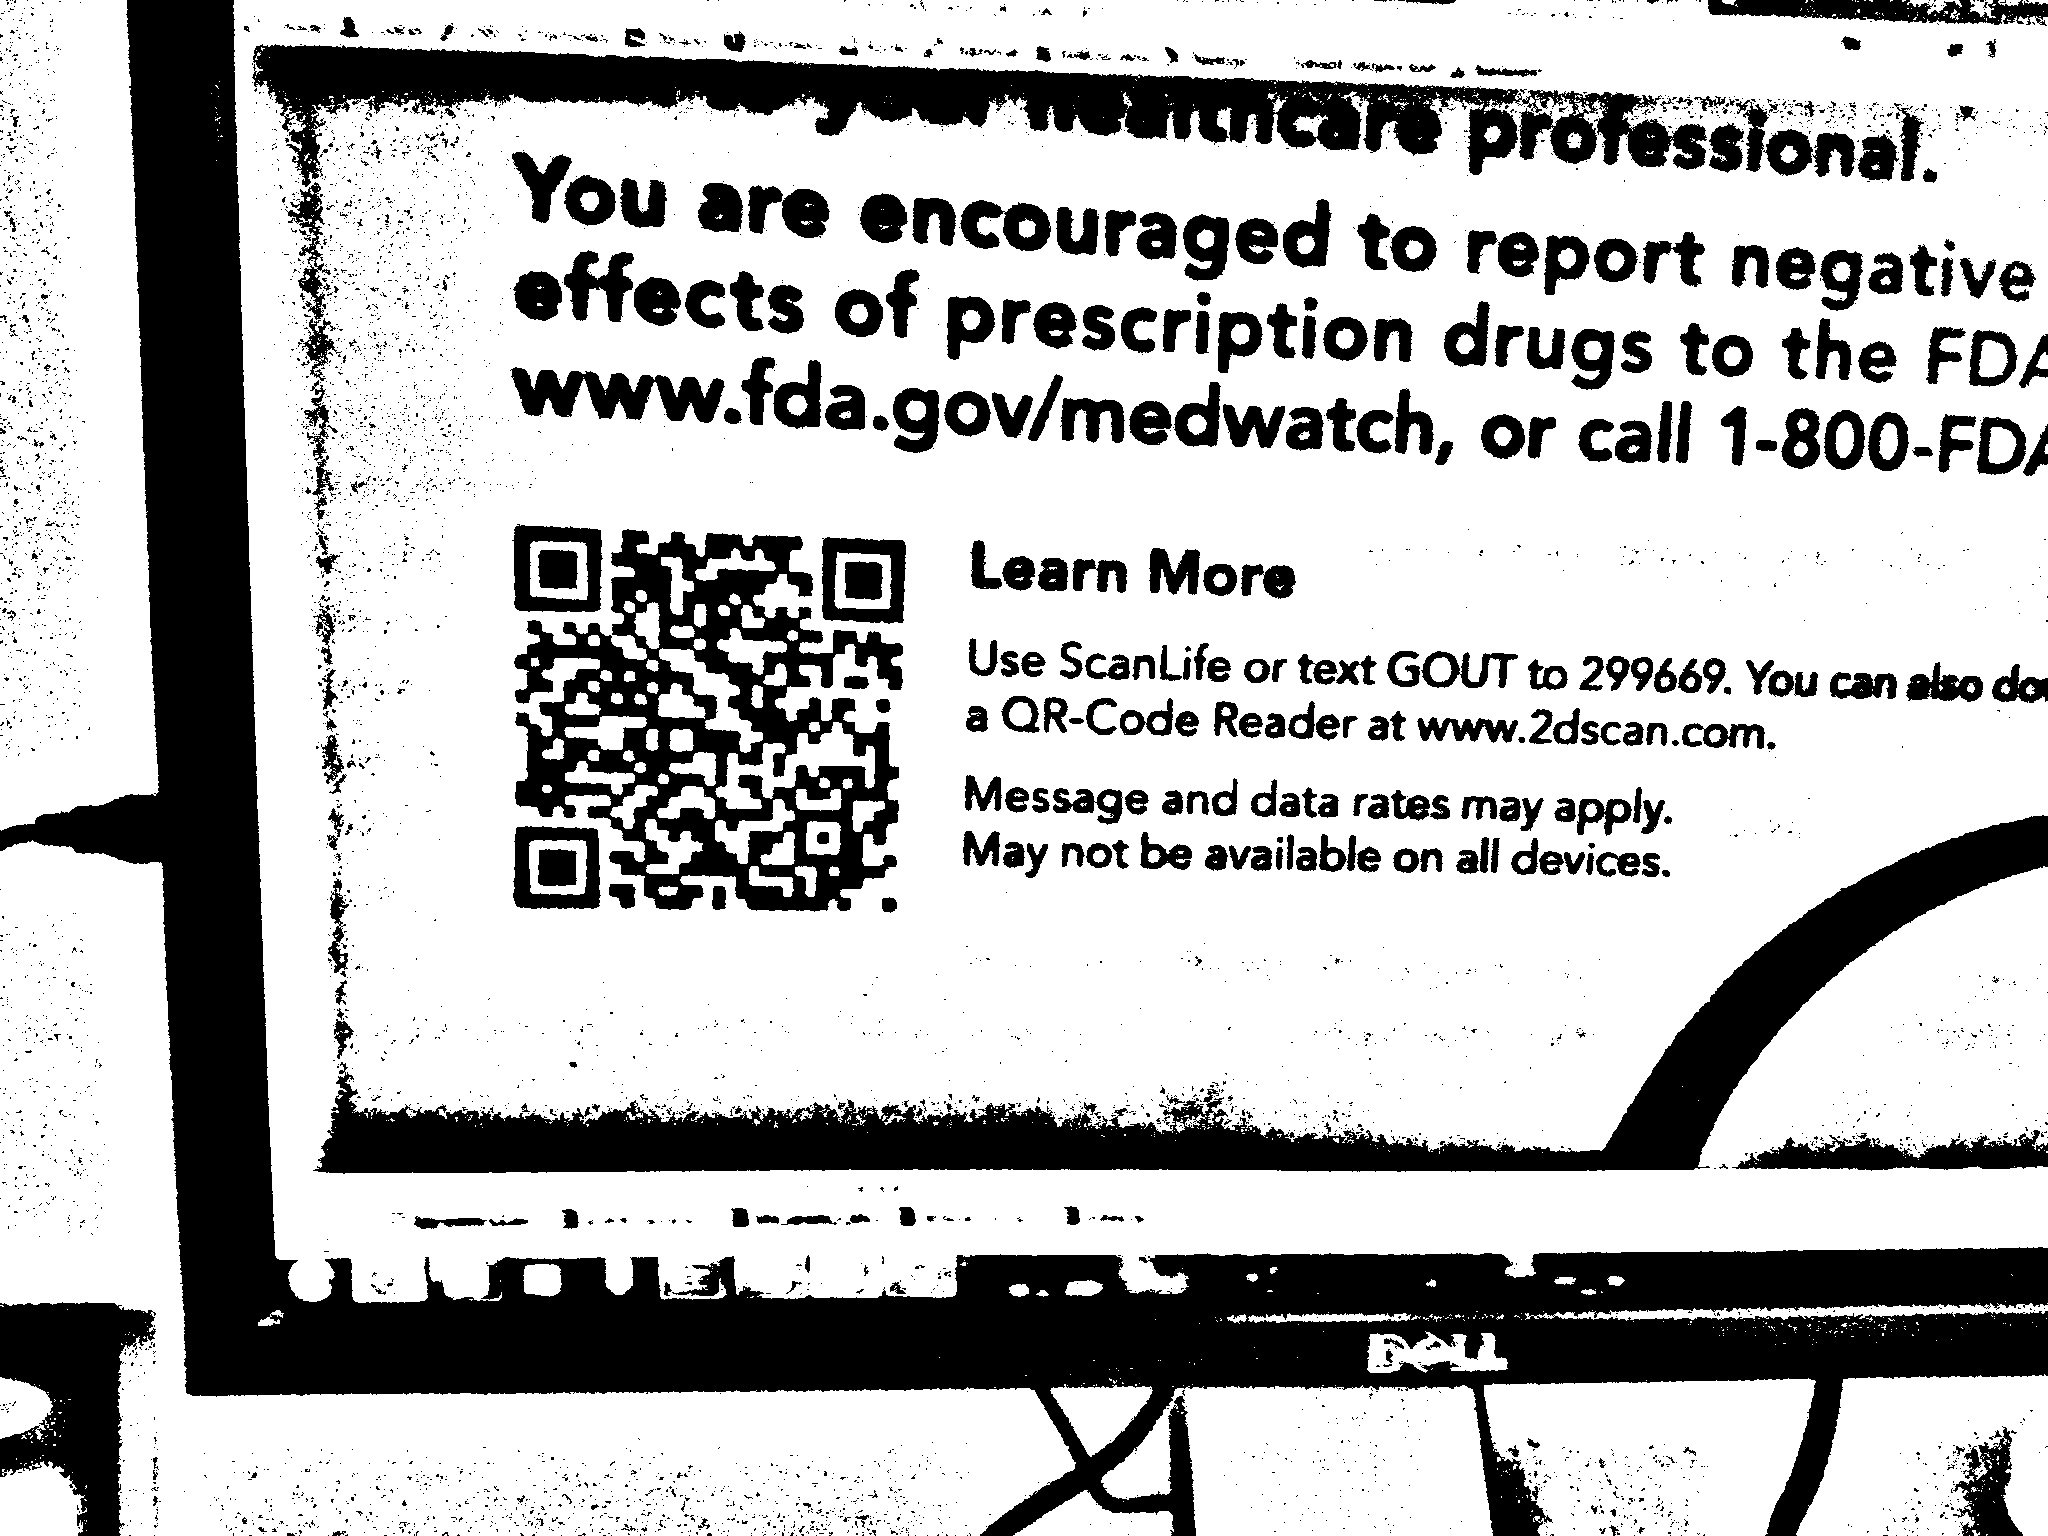
\includegraphics{fig/binarized_2594_7.jpg}
    }
    \caption{Ukázka obrazu se 7000 strukturami}
    \label{SevenThousandsStructures}
  \end{center}
\end{figure}

Pro optimalizaci detekce pozičních značek v reálném obraze, byly přidány další
dva topologické filtry. Ty jsou ovšem volitelné a provádí se pouze při předání
specifické bitové vlajky parametrem \texttt{flags} metodě detekce. Jejich
použití při detekci užité během dekódování by bylo nevhodné, pokud by byl QR kód např.
poškozen a topologická závislost ztracena. První filtr vychází z faktu zmíněného
již během návrhu, že poziční značka musí být tvořena alespoň jednou další
strukturou (menší soustředný čtverec). Druhý filtr je aplikován po detekci první
poziční značky a zjištění její rodičovské struktury, která musí být společná pro
všechny poziční značky.

\subsection{Čtení QR kódu}
\label{cteniQrKoduBarcodesLibr}

Ke čtení QR kódu v obraze slouží singleton třída \texttt{QrDecoder} a její
metoda \texttt{decode()}, jejíž parametry jsou:

\begin{itemize}
  \item \texttt{image} -- vstupní zpracovávaný obraz, který je již ve stupních
  šedi;
  \item \texttt{dataSegments} -- výstupní vektor s přečtenými datovými segmenty;
  \item \texttt{flags} -- doplňující informace ve formě bitových vlajek.
\end{itemize}

Pro čtení byla vytvořena řada pomocných tříd, do kterých byla rozložena vhodně
funkčnost. V jednotlivých krocích čtení se uplatňuje metodika dekódování uvedená
v ISO normě. Jmenujme si proto tyto kroky, v pořadí v jakém jsou aplikovány, a
odpovídající nejzákladnější třídy a metody, které funkčnost implementují.

\subsubsection{Implementace kroků dekódování}

\begin{enumerate}
  \item \textbf{Získání oblasti QR kódu} pro jeho inverzní perspektivní
  transformaci je prováděno pomocí funktorů, jejichž názvy tříd začínají na
  \csuv{\texttt{PerspCornersFrom}}. Byly implementovány celkem tři funktory,
  podle navržených postupů. Selže-li dekódování s jedním funktorem, je vybrán další.
  \item \textbf{Transformace QR kódu} do normalizovaného zobrazení je
  zprostředkována funkcí \texttt{warpPerspective}. Po jejím dokončení je nutno
  QR kód opět binarizovat statickou metodou \texttt{QrDetector::binarize()}.
  Binarizace tentokrát proběhne podle experimentálně získané referenční závislosti a nikoliv v závislosti na předpokládané vzdálenosti QR kódu v obraze. V normalizovaném zobrazení QR kód tedy vyplňuje celý obraz.
  \item \textbf{Zjištění verze QR kódu} z obrazu je důležité pro sestrojení
  čtecí mřížky, je implementováno třídou \texttt{QrVersionInformation} a
  statickou metodou \texttt{fromImage()}, která vrací instanci této třídy.
  \item \textbf{Získání modulů QR kódu} při znalosti verze QR kódu se provádí
  \csuv{přiložením} čtecí mřížky nad QR kód ve statické metodě
  \texttt{BitMatrix::fromImage()}, díky níž získáme reprezentaci QR kódu v
  matici booleovských hodnot.
  \item \textbf{Zjištění formátu QR kódu} je docíleno již z bitové matice
  získané v předešlém kroku a implementováno statickou metodou
  \texttt{QrFormatInformation::fromBitMatrix()}, \linebreak[5]která vrací
  podobně jako u verze instanci této třídy.
  \item \textbf{Maskování dat QR kódu} je uskutečněno sestavením masky
  podle velikosti a formátu QR kódu instancí třídy
  \texttt{QrFormatInformation} a metodou \texttt{buildXORDataMask()}. Operaci
  maskování implementuje třída \texttt{BitMatrix}.
  \item \textbf{Extrakce sekvence dat} a korekce chyby z QR kódu je zařízena
  metodou \texttt{sample()} třídy \texttt{GridSampler}, která
  vzorkuje bitovou matici menší maticí, v našem případě o~velikosti kódového
  slova QR kódu.
  Sekvence jsou získány z kódu ve formě bitového pole \texttt{BitArray}.
  \item \textbf{Uspořádání sekvence dat} a korekce chyby do bloků je zapotřebí z
  důvodu prokládání kódových slov a zpřístupnění opravy chyb, která probíhá vždy
  nad těmito menšími bloky. Za tímto účelem byla vytvořena třída
  \texttt{QrCodewordOrganizer}.
  \item \textbf{Oprava případných chyb} v jednotlivých blocích je realizována s
  pomocí open source Reed-Solomon knihovny napsané v jazyce Java
  \cite{reedSolomonProject}, která byla do jazyka C++ portována. K opravení chyb můžeme přistoupit prostřednictvím
  třídy \texttt{QrReedSolomon}.
  \item \textbf{Dekódování dat} z fyzické vrstvy QR kódu je umožněno třídou
  \texttt{QrBitDecoder}, která shromažďuje a v případě potřeby využívá instance
  implementovaných dekodérů různých režimů. Při dekódování se využívá proudu
  bitů zprostředkovaným třídou \texttt{BitStream}, přičemž bitový proud je
  ustanoven nad přečteným polem bitů \texttt{BitArray}.
\end{enumerate}

\clearpage
\section{Aplikace čtečky QR kódů}

Aplikace čtečky QR kódů byla implementována v jazyce Java pro cílovou platformu
Android. Ke své činnosti využívá výše popsanou C++ knihovnu (kapitola
\ref{knihovnaBarcodesLibrary}), se kterou komunikuje skrze JNI.

Uživatelsky viditelná část aplikace se skládá ze sedmi Activity komponent
(kapitola \ref{aplikaceComponents}). Z důvodů popsaných v návrhu implementuje
aplikace i mechanismus dekódování aplikační vrstvy QR kódů (kapitola
\ref{aplikaceDekodovani}), který je postaven na možnosti snadného přidávání
nových dekodérů do aplikace i včetně skrze zásuvné moduly.

Jelikož některé akce v aplikaci využívají veřejných Intent požadavků aplikace
OI File Manager, je doporučené mít tuto aplikaci pro zkvalitnění práce se
čtečkou QR kódu nainstalovanou.

\subsection{Komponenty aplikace}
\label{aplikaceComponents}

Aplikace je tvořena převážně Activity komponentami.

Hlavní spouštěcí Activity komponentou je \texttt{MainActivity}, která v sobě
implementuje funkčnost zobrazení náhledu z kamery a volání nativních funkcí skrze JNI
rozhraní. Probíhá zde jak detekce, tak i dekódování QR kódu z obrazu, přičemž
obě tyto činnosti běží ve svém vlastním vlákně. V případě detekce je z kamery
přebírán RAW obraz ve formátu NV21, který je převáděn v nativní funkci do
stupňů šedi. Jelikož je NV21 nejčastějším formátem pro náhled, se kterým se
u zařízení pracujících na platformě Android můžeme setkat, nejsou žádné další
formáty aktuálně podporovány. Obraz pro dekódování QR kódu je získáván
z~callback funkce volané z API Androidu při požadavku o sejmutí obrazu. Tato funkce vrací komprimovaný obraz ve formátu JPEG, který je opět v nativní
funkci rozhraní převáděn do stupňů šedi.

Pokud \texttt{MainActivity} komponenta nalezne QR kód a dekóduje jeho fyzickou
vrstvu, je obraz a serializovaný objekt obsahující data QR kódu uložen do
souborů v privátní složce aplikace a zavolána komponenta
\texttt{OpenQrActivity}, které jsou Intent požadavkem předána umístění obou
souborů. Komponenta \texttt{OpenQrActivity} slouží pro dekódování aplikační
vrstvy a zobrazení obrazovky s výsledkem dekódování. Problematika dekódování je blíže
popsána v následující kapitole \ref{aplikaceDekodovani}.

\bigskip \noindent Dalšími spíše doplňkovými Activity komponentami jsou:

\begin{itemize}
  \item \texttt{SettingsActivity} -- implementuje nastavení aplikace, zejména
  škálovatelnost rozlišení a kvality obrazu pro náhled z kamery a snímaného obrazu v JPEG formátu. Dalšími užitečnými volbami může být zapnutí automatického zaostřování nebo blesku pro snímání obrazu aj.;
  \item \texttt{InstallationManagerActivity} -- slouží pro správu a instalování
  nových zásuvných modulů;
  \item \texttt{BrowseImagesActivity} a \texttt{BrowseQRCodesActivity} --
  komponenty jsou určeny pro procházení uložených QR kódů a sejmutých obrazů, příp. pro jejich správu skrze OI File Manager;
  \item \texttt{AboutActivity} -- komponenta zobrazuje informativní obrazovku o
  aplikaci.
\end{itemize}

\subsection{Dekódování aplikační vrstvy QR kódů}
\label{aplikaceDekodovani}

Dekódování aplikační vrstvy QR kódu se provádí po předání kódu Intent požadavkem 
komponentě \texttt{OpenQrActivity}. V níž je dále volána ze singleton třídy
\texttt{QrDecoderManager} metoda \texttt{decode()}, která vrací objekt
reprezentující specifický QR kód.

Proces dekódování je založen na postupném vybírání všech dostupných dekodérů a
testování dekódování pomocí každého z nich, dokud není QR kód úspěšně dekódován.
K~urychlení a zamezení nevhodnému testování dekodérů byla přidána možnost
informování o podporovaných URI schématech, kterými dekodér disponuje. Pokud je
ovšem dekodér \csuv{binární} a nepodporuje URI schémata, nic jiného než
testování nám nezbývá.

Aktuálně jsou v aplikaci zahrnuty pouze dva dekodéry
\texttt{BaseQrDecoder} a \texttt{TextDecoder}. \texttt{BaseQrDecoder}
implementuje dekódování následujících URI schémata: \texttt{http},
\texttt{mailto}, \texttt{tel}, \texttt{URLTO}, \texttt{sms}, \texttt{SMSTO}.
\texttt{TextDecoder} není dekodérem URI schémat a slouží pro dekódování prostého
textu, tudíž má i nejnižší prioritu ze všech dekodérů, neboť většina dnešních
přenosových protokolů je právě textového formátu.

Po dokončení dekódování bylo nutné řešit reprezentaci získaného objektu QR kódu
na obrazovce v podobě pohledu \texttt{View}. Pro tento účel byl implementován
registr adaptérů \texttt{AdapterRegistry} (obrázek \ref{adapterPattern}). Adaptéry jsou
zde určeny k převodu specifického QR kódu na jeho odpovídající pohled, přičemž chceme-li daný
adaptér vyhledat, musí být registrován v registru. Nejpodstatnější metodou
adaptéru je metoda \texttt{getProvider()}, která vrací samotný objekt
zprostředkovávající převod, konkrétně objekt implementující rozhraní
\texttt{QrCodeViewProvider}. Celkově byly implementovány adaptéry pro zobrazení
QR kódů obsahujících SMS, e-mailu, tel. čísla, internetové stránky a prostého textu.
 
 \begin{figure}[H]
  \begin{center}
    \scalebox{0.35}{
      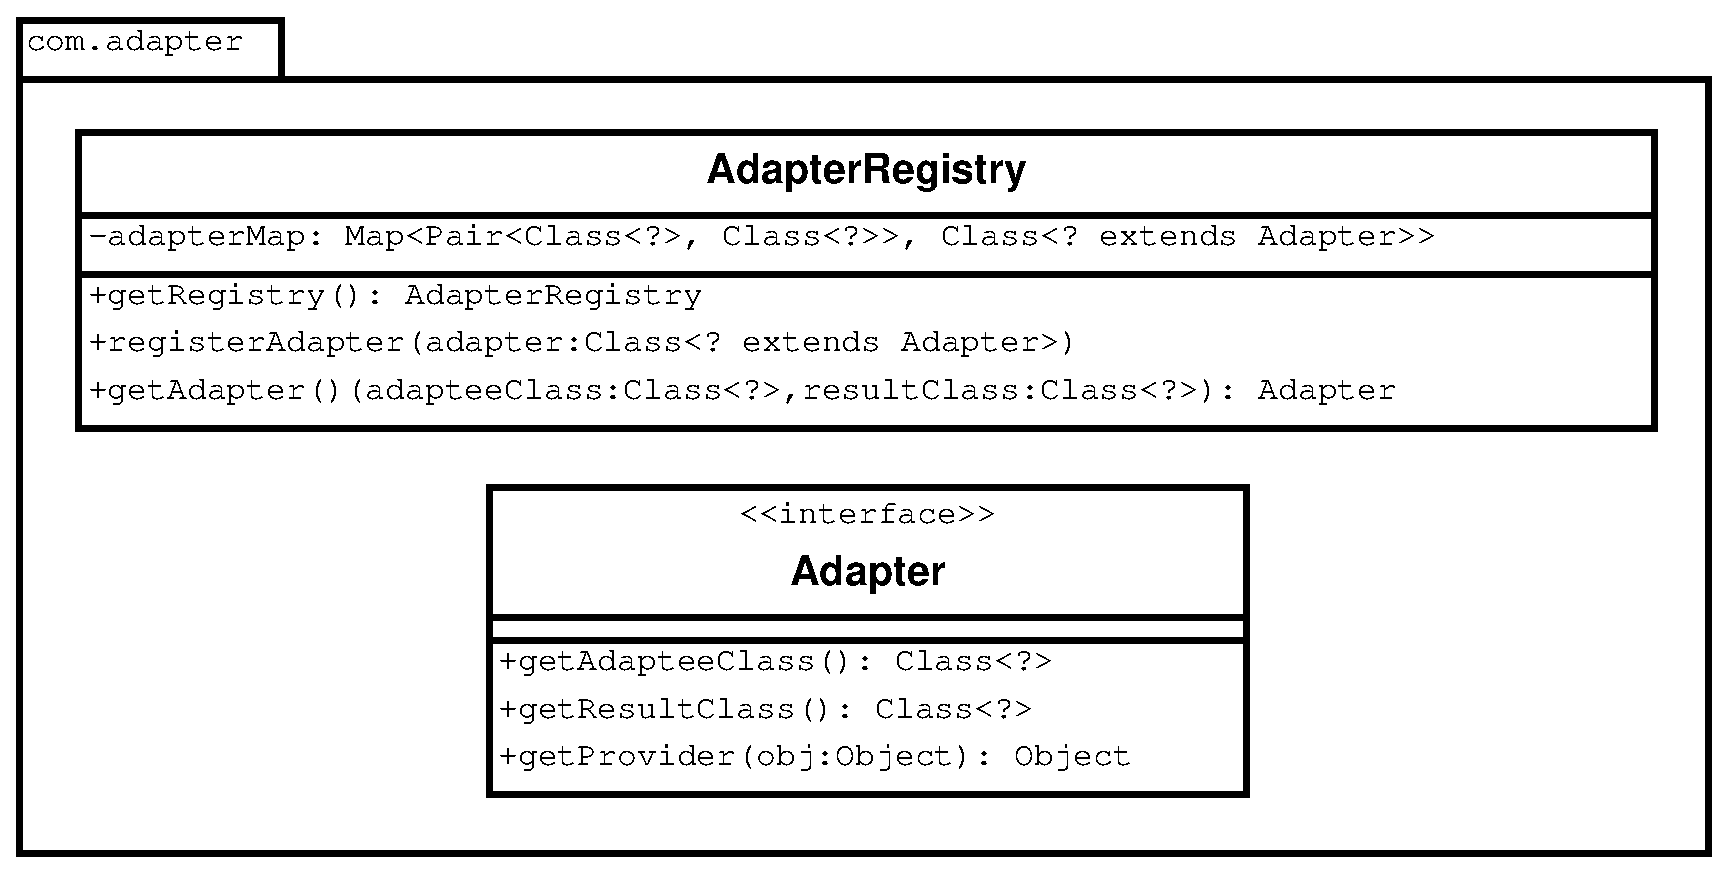
\includegraphics{fig/adapter.eps}
    }
    \caption{Registr adaptérů využitý pro mapování QR kódů na odpovídající
    pohledy}
    \label{adapterPattern}
  \end{center}
\end{figure}
 
Pro snadné přidávání dekodérů aplikační vrstvy, pouhým rozšířením pole
dostupných dekodérů, a pohledů QR kódů, zaregistrováním v registru adaptérů,
byla přidána podpora zásuvných doplňků v aplikaci.

Zásuvný doplněk je prostý JAR archiv, který obsahuje zkompilované třídy ve
formátu Dalvik Executable a ve složce \texttt{res} dva popisné XML soubory.
První XML soubor \texttt{package.xml} sděluje informace o doplňku, aktuálně pouze jeho
název a základní popis. Druhý XML soubor \texttt{classes.xml} říká třídě
spravující doplňky \texttt{InstallationManager}, které třídy jsou obsažené v
archivu a mají být načteny. Správce doplňků dále využívají specializované třídy
pro načítání nových dekodérů \texttt{InstallableQrDecoderManager} a pro načítání
pohledů \texttt{InstallableQrCodeViewManager}.


\chapter{Dosažené výsledky}
\label{vysledky}

V této kapitole bude zhodnocena výkonnost a spolehlivost implementovaného
řešení detekce a čtení QR kódů. Závěrem budou diskutovány budoucí možná
rozšíření aplikace.

Pro vyhodnocení spolehlivosti a výkonnosti aplikace byly použity výbavou velmi
odlišné mobilní telefony Samsung S5570 Galaxy Mini (dále pouze 
\csuv{Samsung}) a LG P990 Optimus 2X (dále pouze \csuv{LG}). Telefon LG,
díky svému dvoujádrovému procesoru a kvalitnímu 8 Mpix fotoaparátu, dosáhl v
následujících testech značně lepších výsledků než telefon Samsung.

\section{Vyhodnocení spolehlivosti}

Spolehlivost čtečky QR kódů je dána především kvalitou vstupního obrazu. Bylo
zjištěno, že největší negativní vliv na čtení má rozostřený obraz. Bílé moduly
QR kódu jsou potom během binarizace umocňovány, což způsobuje někdy až ztrátu
modulů tmavých. Ačkoliv ztracené moduly v QR kódu mohou být často opraveny,
problém ovšem nastává při neostrých pozičních značkách, které musí splňovat pro
úspěšnou detekci 80\% shodu v šablonovém porovnání. Při čtení QR kódu z malé
vzdálenosti se ale s předchozími problémy nesetkáme. Výjimku tvoří pouze QR
kódy nejvyšších verzí, kde poziční značky zabírají velmi malou část obrazu i z
blízka sejmutého obrazu. Takové kódy se ovšem v praxi téměř vůbec nepoužívají.

Čtečka si umí dobře poradit s QR kódy, které jsou sejmuty při špatných
světelných podmínkách. Pokud je QR kód poškozen je použita Reed-Solomonova
metoda k jeho opravení (obrázek \ref{readableCodes}).

 \begin{figure}[H]
  \begin{center}
    \scalebox{0.31}{
      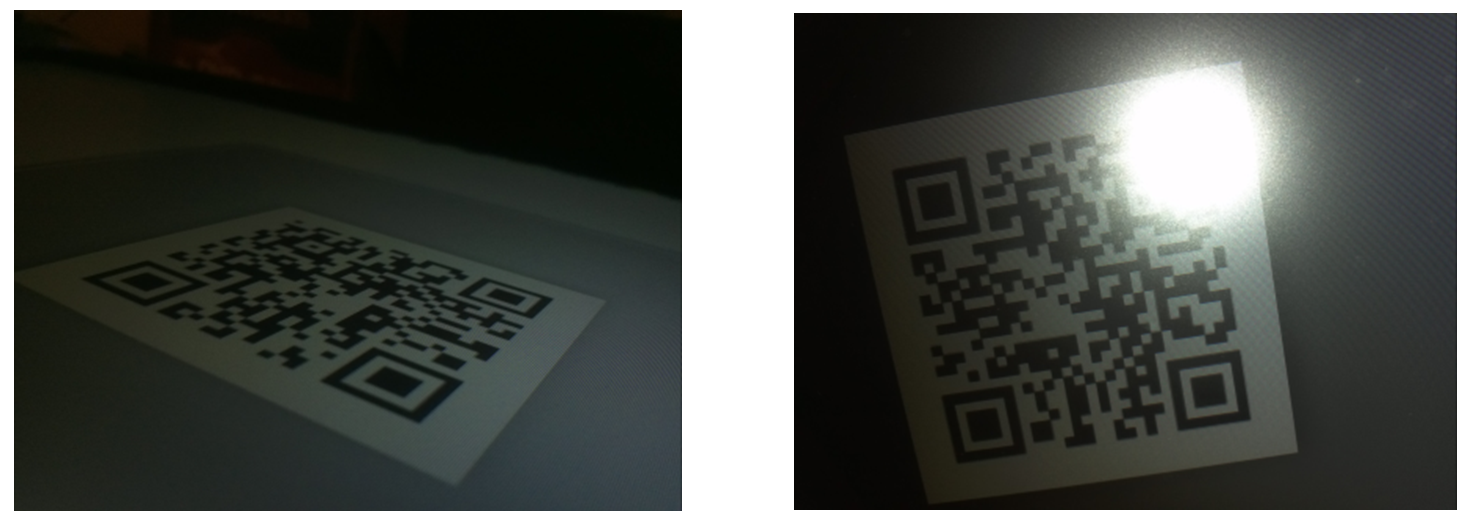
\includegraphics{fig/readableCodes.PNG}
    }
    \caption{Čitelný a opravitelný QR kód}
    \label{readableCodes}
  \end{center}
\end{figure}

Při detekci QR kódu a transformaci do
normalizovaného zobrazení není čtečka závislá na nalezení zarovnávacích značek,
tak jako všechny ostatní testované čtečky QR kódů
\cite{barcodeReaderZxing,scanLife,qrReaderForAndroid}. Selže-li ovšem čtení s
jednou metodou transformace, je využito i metody založené na nálezu zarovnávacích značek. Nachází-li se v obraze více QR kódů, čili obsahuje více
než 3 poziční značky, snaží se čtečka tyto poziční značky uskupit tak, aby
alespoň jeden z kódu mohl být dekódován. Podmínkou ovšem zůstává, že kódy musí
být ohraničeny. Čtečkou mohou být čteny i vzdálené QR kódy, musí být ale splněna
minimální velikost stran minimálního ohraničujícího obdélníku poziční značky
(kapitola \ref{optimalizaceDetekce}). Pro čtení tato velikost je 14 pixelů.

Naopak čtečka si neumí poradit s QR kódy, které jsou např. vylepené na
zakřiveném povrchu láhve. S telefonem Samsung se nepodařilo řádně přečíst QR kód
nejvyšší verze, pouze ho detekovat. Telefon LG si s tímto kódem poradil, ale
pouze až s využitím automatického zaostření. Jakékoliv porušení struktury
poziční značky, vedoucí např. k nalezení 5. rohu poziční značky nebo spojení
dvou struktur, způsobí neúspěšnou detekci QR kódu v obraze.

\section{Vyhodnocení výkonnosti}

Při vyhodnocování výkonnosti byla zkoumána celková doba, jaká je potřebná pro
provedení detekce QR kódu v reálném obraze a jeho čtení v sejmutém obraze.
Hlavním faktorem ovlivňujícím výkonnost bylo dle očekávání rozlišení
zpracovávaného obrazu. Referenčním použitý obraz pro testování obsahoval
neporušený QR kód verze 3.

Ke změření závislosti doby detekce pozičních značek na velikosti obrazu, bylo
proměnlivě nastavováno rozlišení náhledu z kamery, který je k detekci využíván.
Doba byla odečítána pomocí systémového času, nikoliv procesorového, tudíž jí
lze použít i k příp. převodu na zpracované rámce za sekundu. Získanou závislost
lze vidět v grafu na obrázku \ref{detectionFPS}. Při výchozím nastavení
rozlišení náhledu, tzn.
rozlišení odpovídajícímu rozlišení displeje, bylo u obou přístrojů dosaženo
frekvence obnovy volání detekce 5-6 rámců za sekundu. Jediným faktorem, který
může frekvenci v daném rozlišení výrazně ovlivnit je počet detekovaných struktur
v rámci metody detekce. Není-li obraz strukturovaný, lze pozorovat při výchozím
rozlišení zpracování až 10 rámců obrazu za sekundu, v opačném případě naopak
výrazně méně.

 \begin{figure}[H]
  \begin{center}
    \scalebox{0.53}{
      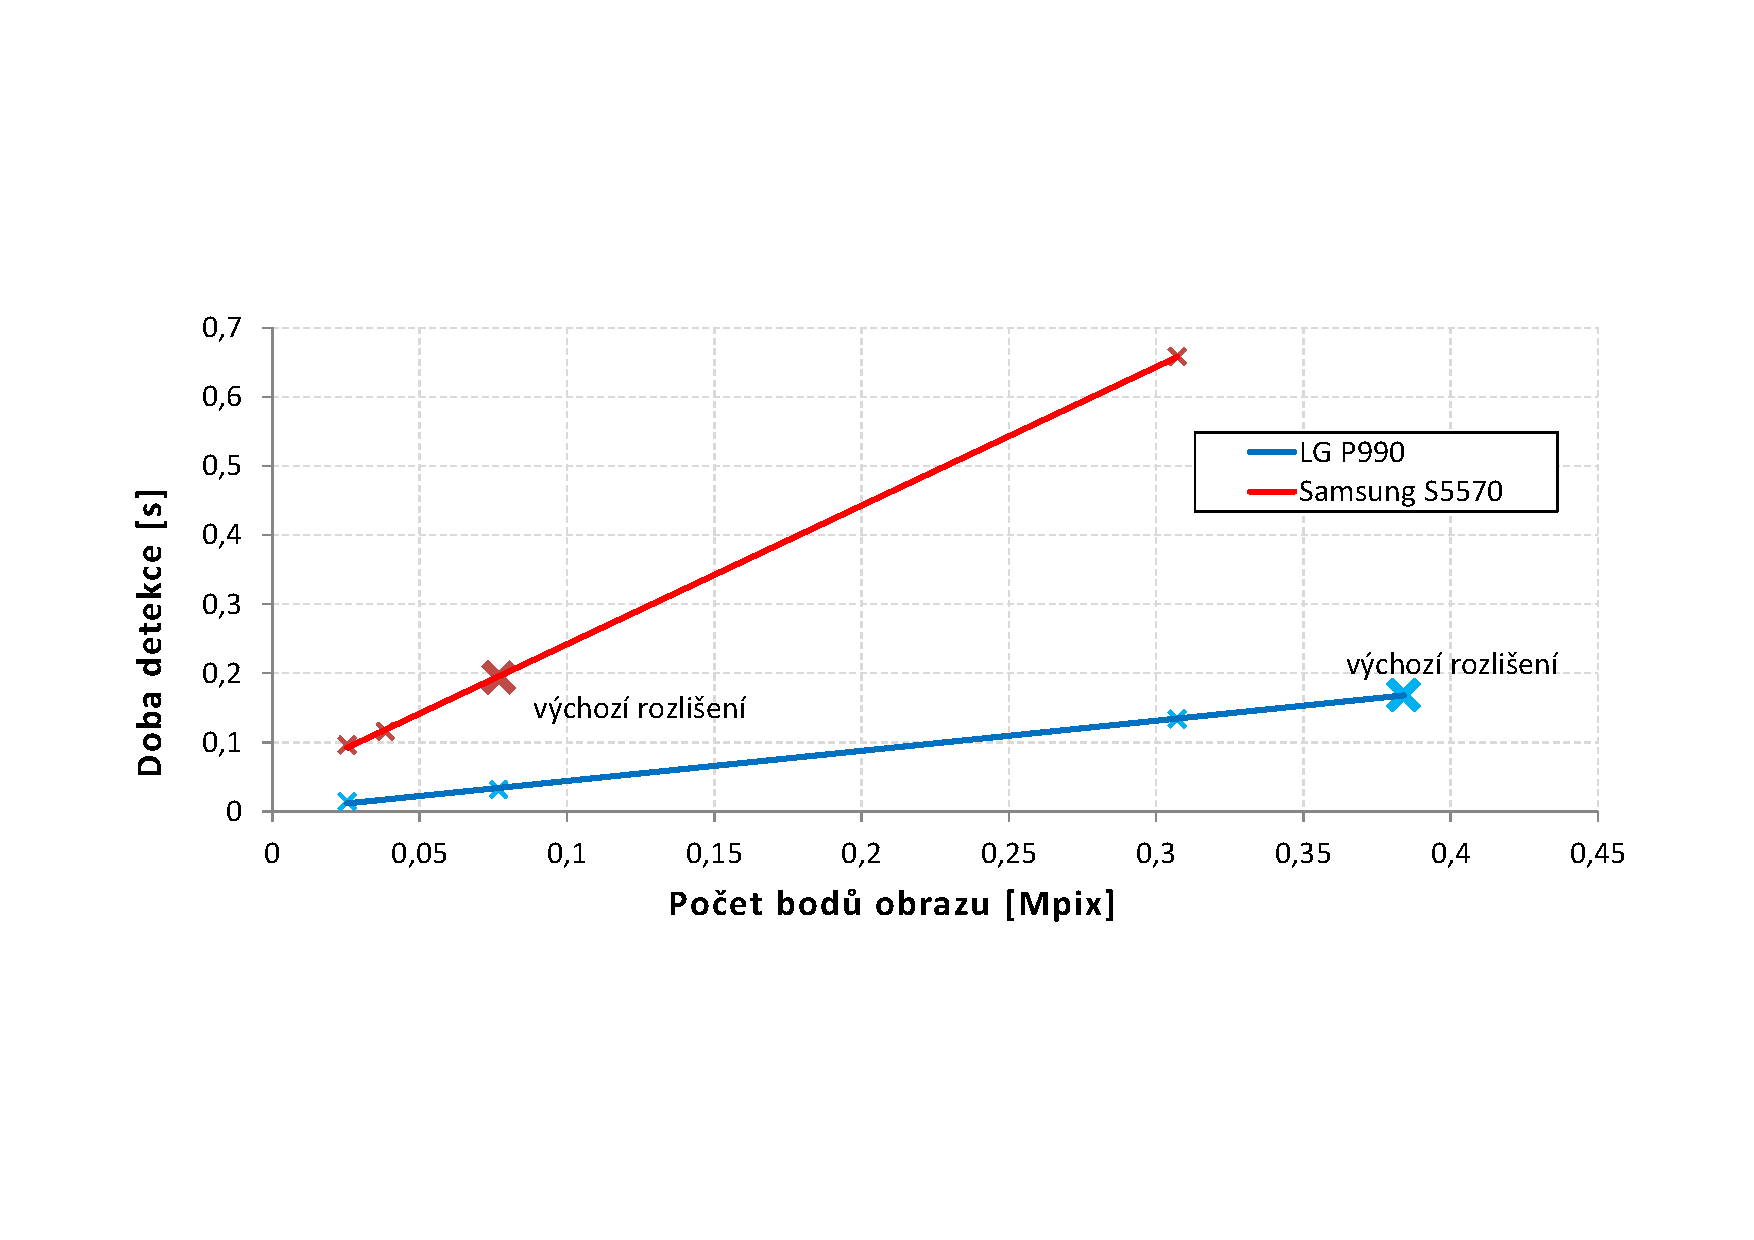
\includegraphics[trim = 1.5cm 5cm 1.5cm 5cm]{fig/detectionFPS.pdf}
    }
    \caption{Graf závislosti doby detekce pozičních značek na velikosti obrazu}
    \label{detectionFPS}
  \end{center}
\end{figure}

Vyhodnocení výkonnosti čtení probíhalo obdobným způsobem jako u detekce
pozičních značek, pouze s tím rozdílem, že rozlišení nebylo proměnlivě
nastavováno náhledu z kamery, ale z kamery sejmutému obrazu. Výkonnost čtení,
které se mj. skládá i z detekce pozičních značek, lze vidět na obrázku
\ref{decodeFPS}.

 \begin{figure}[H]
  \begin{center}
    \scalebox{0.53}{
      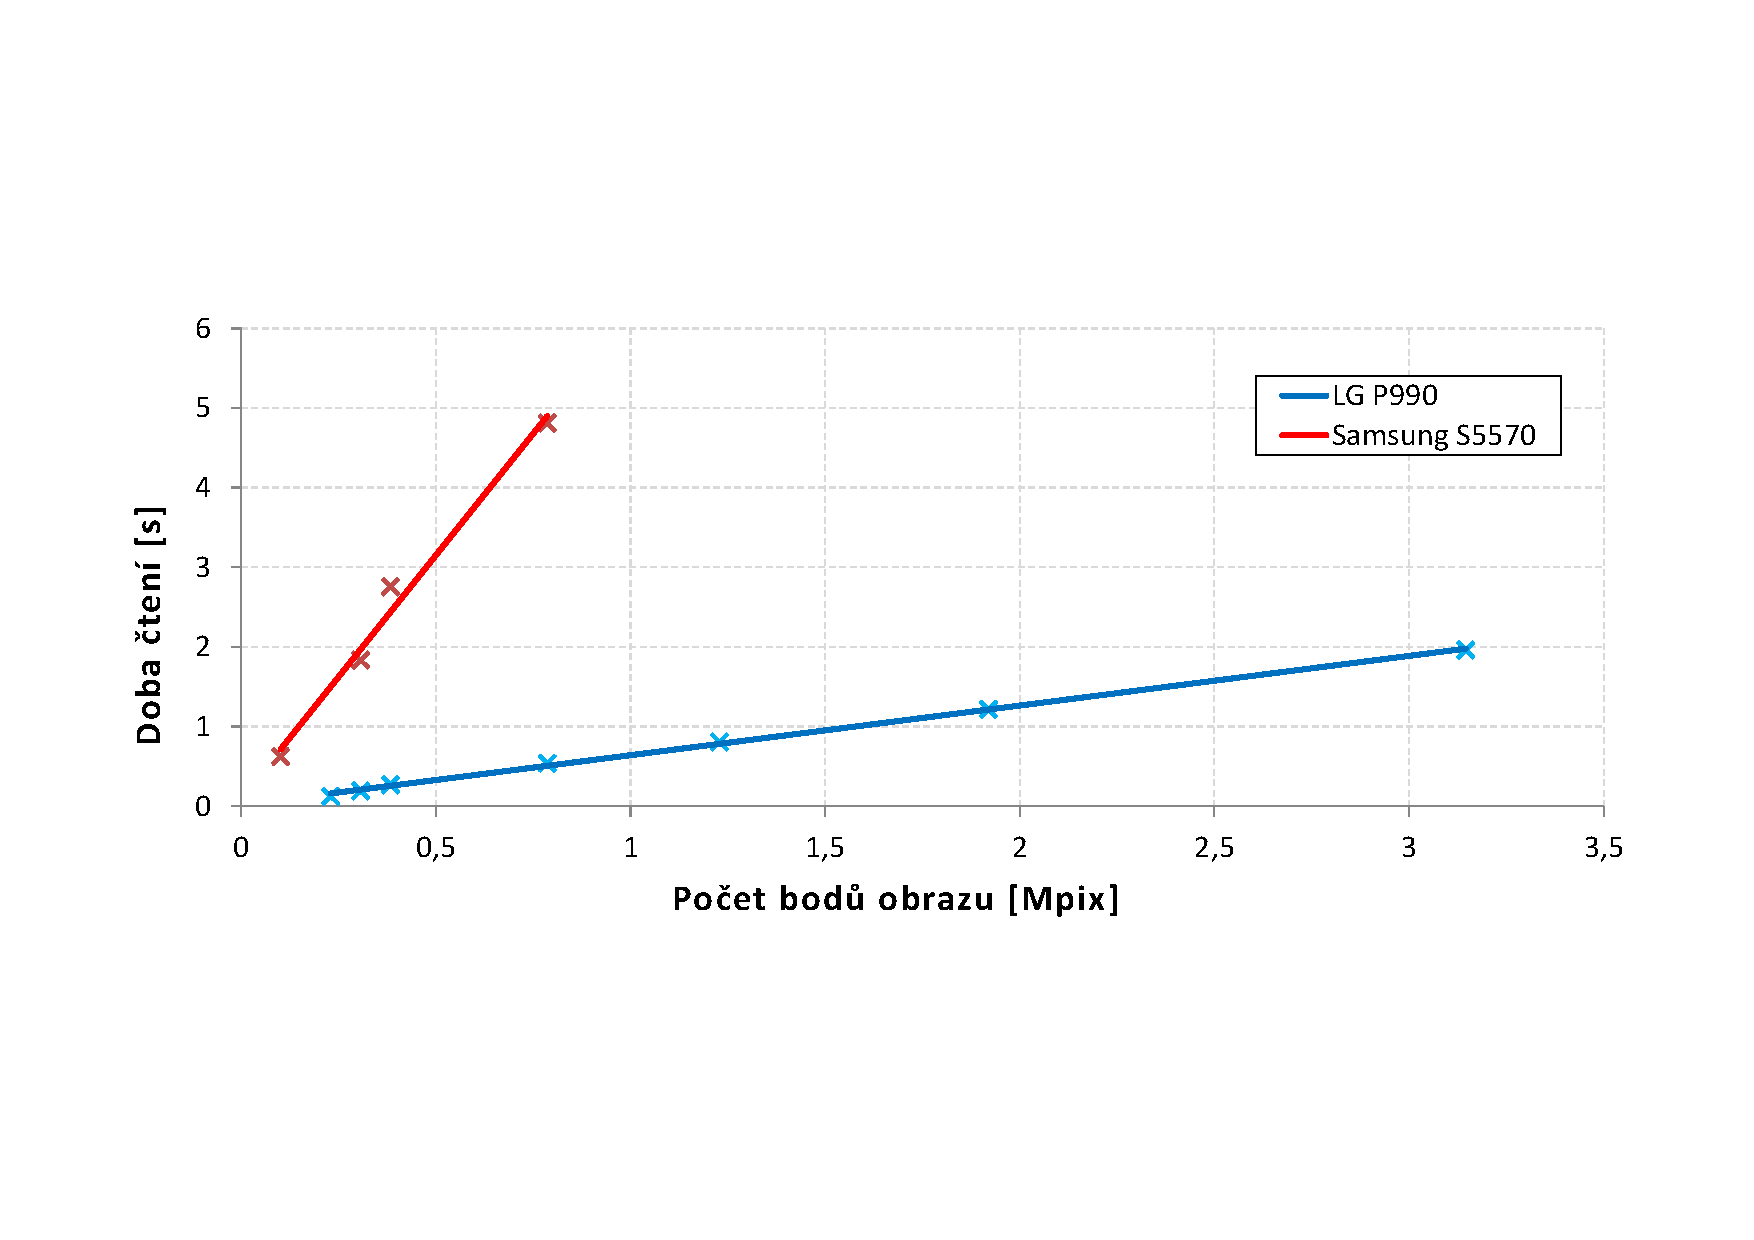
\includegraphics[trim = 1.5cm 5cm 1.5cm 5cm]{fig/decodeFPS.pdf}
    }
    \caption{Graf závislosti doby čtení QR kódu na velikosti obrazu}
    \label{decodeFPS}
  \end{center}
\end{figure}

Jelikož proces čtení QR kódu se skládá z více kroků, byla provedena analýza
stráveného procesorového času uvnitř jednotlivých kroků (obrázek
\ref{decodingStepsOverview}). Výsledku může být využito v budoucnu pro návrh
případných optimalizací.

 \begin{figure}[H]
  \begin{center}
    \scalebox{0.50}{
      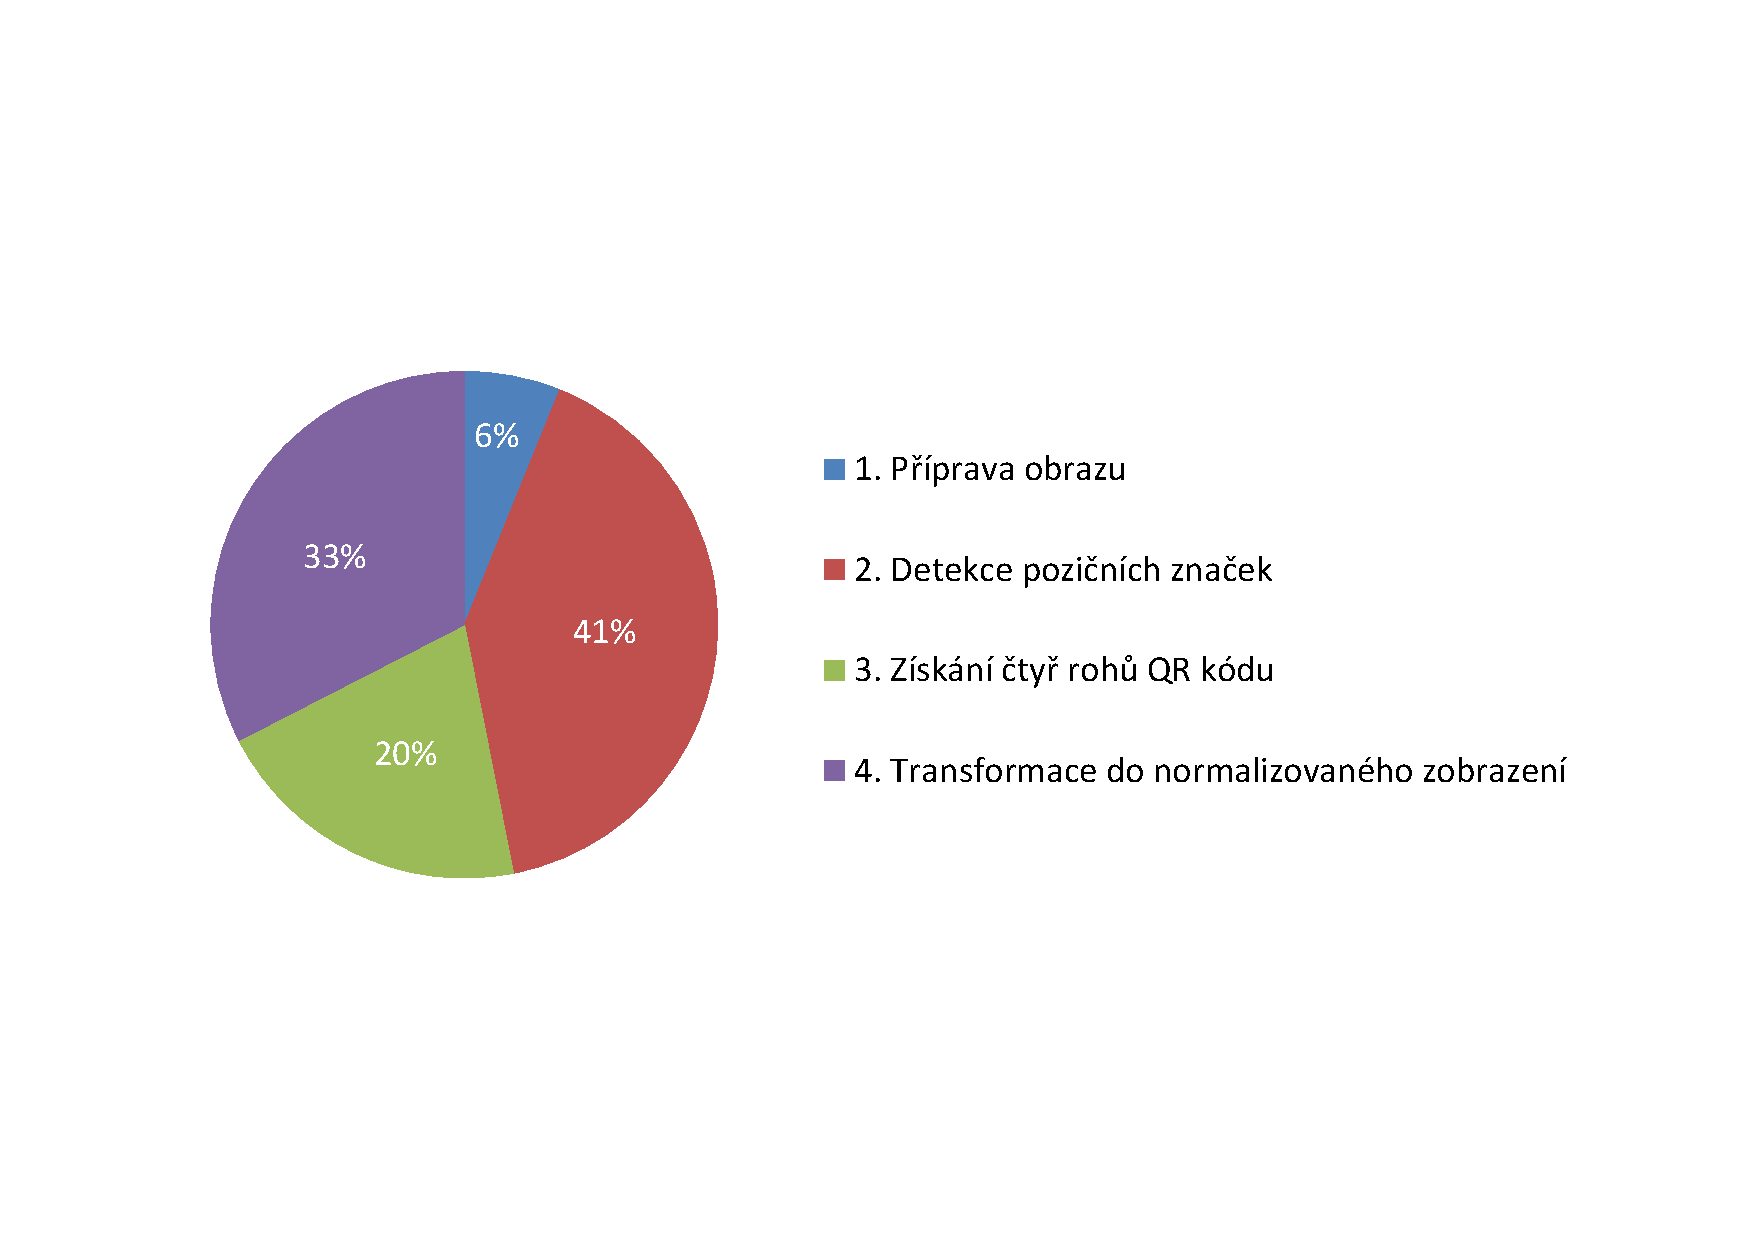
\includegraphics[trim = 2.5cm 5cm 3.5cm
      5cm]{fig/decodingStepsOverview.pdf} }
    \caption{Graf procesorového času stráveného v jednotlivých
    krocích čtení QR kódu}
    \label{decodingStepsOverview}
  \end{center}
\end{figure}

Bylo zjištěno, že převážná část procesorového času je spotřebována právě v kroku
detekce pozičních značek. Následně po ní se ukázal být náročný krok transformace
QR kódu do normalizovaného zobrazení. Avšak ne samotná transformace, ale
binarizace obrazu, která je prováděna ihned po transformaci v témže kroku.
Překvapivě dobře dopadl krok přípravy obrazu, ve kterém je převáděn komprimovaný
obraz v JPEG formátu na obraz ve stupních šedi. Další kroky čtení, které nejsou
v kruhovém grafu uvedeny, ukrojily z celkového času pouhých 0,1%.

\section{Možnosti budoucího vývoje}

Velkým prostorem pro samotný vývoj se skýtá v C++ knihovně pro detekci a čtení
QR kódů. Knihovnu by bylo možné rozšířit např. o podporu čtení Micro QR kódů,
strukturovaného režimu nebo kódů ze zakřivených povrchů.

Přidání podpory pro čtení skupiny Micro QR kódů by znamenalo pouze změnit
koncepci nacházení oblasti QR kódu. Ta by mohla být založena na sledování
synchronizačních vzorů vedoucích z detekované poziční značky Micro QR kódu
(\ref{microQRCodePoints}).
Pokud by sledování dosáhlo konce, tzn. strany QR kódu, byly by zde stanoveny
rohy A a C. Tyto rohy by se staly zároveň i počátečními body pro vzorkování a
nalezení čtvrtého rohu QR kódu D -- viz kapitola \ref{zjisteniATransformace}.

 \begin{figure}[H]
  \begin{center}
    \scalebox{0.18}{
      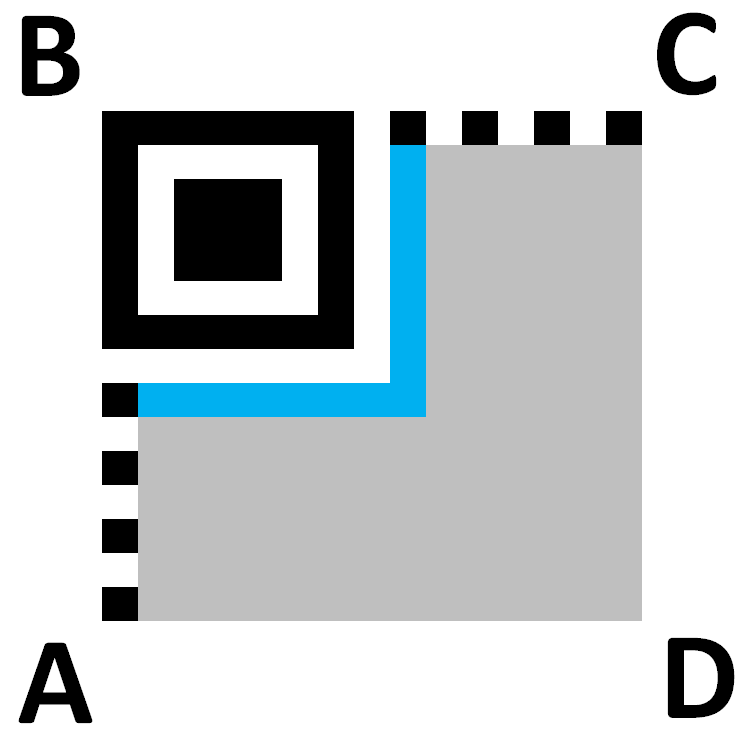
\includegraphics{fig/microQRCodePoints.PNG}
    }
    \caption{Micro QR kód}
    \label{microQRCodePoints}
  \end{center}
\end{figure}

Podpora strukturovaného režimu (kapitola \ref{kodovaniDat}) nebyla pozorována na žádné z
testovaných veřejně dostupných čteček pro platformu Android. Režim  slouží pro umístění
dat do více QR kódů (obrázek \ref{qrdiv}). Využívá se spíše v aplikačně
uzavřených doménách např. pro značení výrobků s nedostatečným prostorem pro tisk v obou
dimenzích. Hlavním problémem, který se zde vyskytuje, je rozlišení pozičních
značek a přiřazení k jednotlivým QR kódům. Implementačně by se to dalo řešit
opět sledováním synchronizačních vzorů vedoucích z jednotlivých pozičních
značek. Pokud by ke značce vedly dva synchronizační vzory, byla by tato
značka prohlášena jako levá horní. Aby mohlo být rozhodnuto, že v daném směru
existuje synchronizační vzor, musel by být každý takový vzor zakončen sekvencí
tmavých a světlých modulů poziční značky v poměru 1:1:3:1:1.

 \begin{figure}[H]
  \begin{center}
    \scalebox{0.80}{
      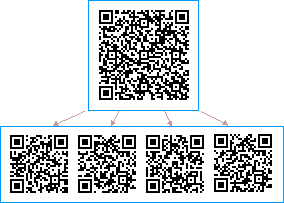
\includegraphics{fig/qrdiv.PNG}
    }
    \caption{Rozdělení dat do více QR kódů pomocí strukturovaného režimu}
    \label{qrdiv}
  \end{center}
\end{figure}

Čtení QR kódů ze zakřivených povrchů by šlo realizovat pomocí zarovnávacích
značek v QR kódu. Samotný princip čtení je dokonce uveden v referenčním
algoritmu pro čtení QR kódů v ISO normě. Podstata by spočívala v nalezení
zarovnávacích značek a rozdělení QR kódu na dvourozměrné menší bloky
(obrázek \ref{alignmentBlocks}), které by poté byly samostatně převedeny
perspektivní inverzní transformací do normalizovaného zobrazení. Po převodu všech bloků by se obraz
sjednotil a mohla by být aplikována standardní metodika čtení.
 
  \begin{figure}[H]
  \begin{center}
    \scalebox{0.25}{
      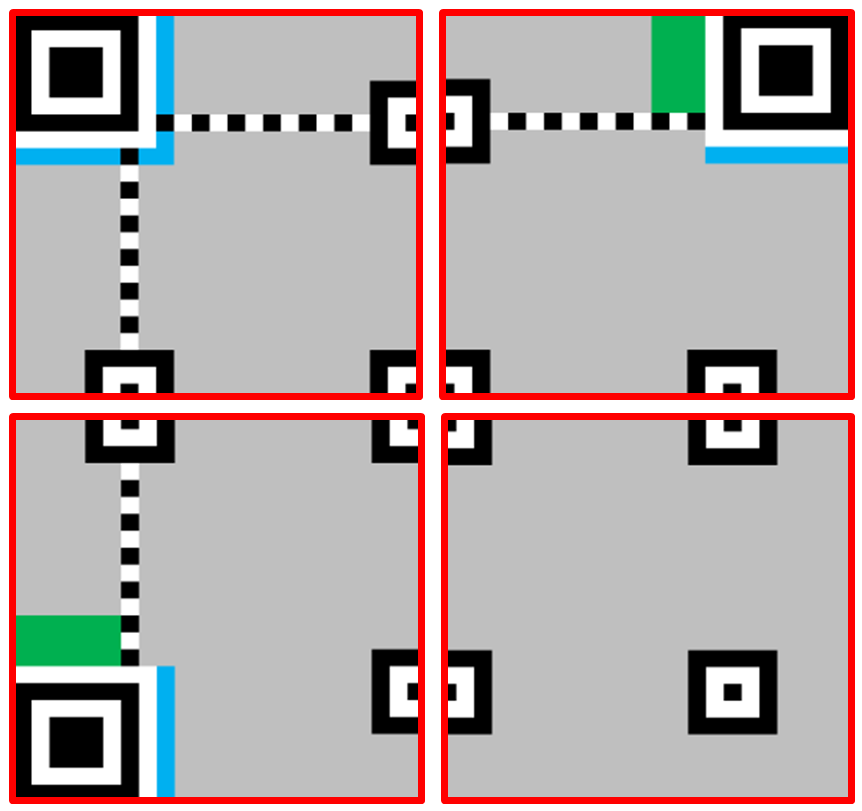
\includegraphics{fig/alignmentBlocks.PNG}
    }
    \caption{Rozdělení QR kódu do bloků podle zarovnávacích značek}
    \label{alignmentBlocks}
  \end{center}
\end{figure}
 
Rozšíření aplikace pro Android by bylo také možné. Zahrnovalo by spíše ale
vylepšení z pohledu uživatele, nikoliv však funkční z pohledu spolehlivosti 
a podpory čtení QR kódů. Hlavním přínosem by byla implementace souborového
správce, který by byl využit pro správu QR kódů, obrázků a instalovaní zásuvných
doplňků. Nyní je za tímto účelem nutno mít nainstalovanou aplikaci OI File
Manager. Procházení složek a souborů je již v aplikaci implementováno, ale není
doplněno o akce správy (mazání, přesouvání apod.). Druhým, implementačně méně
náročným vylepšením, by mohlo být umožnění dekódování QR kódu z fotografie z
jakéhokoliv souborového správce.

\chapter{Závěr}

Cílem této bakalářské práce bylo prozkoumat problematiku dvourozměrných čárových
QR kódů. Na základě získaných teoretických znalostí navrhnout algoritmy pro
jejich automatické rozpoznání a přečtení ve snímaném obraze. Dále tyto algoritmy
implementovat a využít v aplikaci čtečky QR kódů pro mobilní platformu Android.

Během návrhu metodiky čtení QR kódů práce vychází z aktuální normy
spravující standard QR kódů. Pro některé kroky čtení, které norma
nespecifikovala, nebo nebyly pro naše účely příliš vhodné, bylo nutno
prezentovat vlastní řešení. Jedná se zejména o metodu binarizace, lokalizaci QR
kódu v obraze a jeho transformaci do normalizovaného zobrazení.

V praktické části práce byla v jazyce C++ s využitím knihovny OpenCV vytvořena
knihovna, která zajišťuje lokalizaci a čtení QR kódů v obraze. Knihovna je
napsána přenositelně a byla úspěšně otestována na mobilních architekturách
ARMv6 a ARMv7a a desktopových architekturách x86 a x64.

Druhým produktem praktické části práce je aplikace čtečky QR kódů napsaná v
jazyce Java, jejíž funkčnost je závislá na dostupnosti předešlé knihovny.
Samotná knihovna je potom v aplikaci čtečky QR kódů dynamicky načítána. Vzájemná
komunikace mezi aplikací a knihovnou probíhá skrze nativní rozhraní JNI.
Aplikace je unikátní od ostatních čteček QR kódů zejména svojí snadnou
rozšiřitelností v podobě zásuvných doplňků, dokonce i za běhu aplikace.

V rámci práce se podařilo implementovat všechny navržené postupy. Výsledná
aplikace by proto mohla být používána v praxi. Při vytracení zarovnávacích
značek z QR kódů, je aplikace schopna tento kód přesto dekódovat, na rozdíl od
všech testovaných veřejně dostupných čteček, které s tímto měly problém. Z
důvodu nedostatečné rychlosti dekódování a dekódování ve více krocích, které
může nastat při selhání jednoho přístupu a pokusu o nápravu chyby jiným
přístupem, se nedoporučuje používat aplikaci při zpracování QR kódů z reálného
obrazu. Detekce QR kódů v \csuv{běžném} reálném obraze, jehož rozlišení
odpovídalo rozlišení displeje, na testovaných mobilních zařízeních dosahovala
frekvence obnovy 5-6 rámců za sekundu.

Budoucí vývoj práce by mohl spočívat hlavně v optimalizaci a zvýšení přesnosti
lokalizace QR kódů. Mohla by být přidána i podpora čtení více QR kódů v obraze
a nové skupiny QR kódů tzv. Micro QR kódů. Výhodou by byla i schopnost čtení ze
zakřivených povrchů.
